% !TeX TS-program = pdflatex
% !BIB program = biber


\documentclass[a4paper, 10pt]{article}

\newcommand{\papertitle}{Eckstein--Keane--Wolpin models \\
	\Large An invitation for transdisciplinary collaboration}
% !TeX TXS-program:compile = txs:///pdflatex/
% !TeX TS-program = pdflatex
% !TeX TXS-program:bibliography = txs:///biber
% !BIB program = biber




%%%%%%%%%%%%%%%%%%%%%%%%%%%%%%%%%%%%%%%%%
%%  FUNDAMENTAL PACKAGES AND COMMANDS  %%
%%%%%%%%%%%%%%%%%%%%%%%%%%%%%%%%%%%%%%%%%
\usepackage{ifxetex}  % Detect if engine is XeTeX/XeLaTeX
\usepackage{ifthen}

\usepackage[utf8]{inputenc}  % so that umlauts can be input without having to use TeX code

\ifxetex
	\usepackage[euenc]{fontspec}
\else
	\usepackage[LGR, T1]{fontenc}  % LGR needed for sansserif math
\fi

\usepackage[ngerman, american, USenglish]{babel}  % German and US English hyphenation and quotation marks
\selectlanguage{USenglish}
\usepackage[ngerman, USenglish]{isodate}
\usepackage[babel, german=quotes]{csquotes}  % Needed for correct German quotes via BibLaTeX's \mkbibquote{...}
%\usepackage[babel, german=guillemets]{csquotes}  % Needed for correct German quotes via BibLaTeX's \mkbibquote{...}

\usepackage{calc}  % Enables calculations for lengths; provides, e.g., \widthof{text}
\usepackage{fp}  % Enables calculations in LaTeX
% \usepackage[nomessages]{fp}

\usepackage{etoolbox}  % Enables manipulating LaTeX commmands via \preto, \appto, \patchcmd, etc.
\usepackage{xpatch}  % Enables manipulating LaTeX commmands via \xpatchcmd etc.
\usepackage{letltxmacro}
\usepackage{xparse}

%\usepackage{geometry}  % See geometry.pdf to learn the layout options. There are lots.
%\usepackage[mathscr]{eucal}
%\geometry{a4paper, top=20mm, bottom=20mm, right=20mm, left=30mm}
%\geometry{landscape}  % Activate for for rotated page geometry

\usepackage{ragged2e}
% Provides, among others, the \RaggedRight environment, which is \raggedright but with hyphenation enabled.
%\renewcommand{\raggedright}{\RaggedRight}

\usepackage{import}	 % To allow for relative paths in nested \input's (\import's)

% \usepackage{float} % damit die figure da ist wo sie sein soll
\usepackage{placeins}  % Improve placing of floats (figures, tables), provides \FloatBarrier

% DO NOT USE \usepackage{amssymb}!
% The AMS symbols are included in the mathdesign package or the fourier package.
\usepackage{amsmath}
\MakeRobust{\eqref}
	% See https://tex.stackexchange.com/questions/61764/eqref-in-captions-with-mathtools
\renewcommand{\eqref}[1]{(\ref{#1})}  % Necessary to make the font switch from serif to sansserif where required.
\usepackage{amsthm}	% provides \newtheoremstyle
\usepackage{mathtools}
%\mathtoolsset{centercolon}
	% This makes the compilation fail in combination with tikz. See
	% https://tex.stackexchange.com/questions/89467/why-does-pdftex-hang-on-this-file.
% Inspired by https://tex.stackexchange.com/questions/251460/how-to-put-symbols-of-equal-size-on-top-of-each-other
\newcommand{\succeqq}{%
  \mathrel{%
    \vcenter{\offinterlineskip
      \ialign{##\cr$\succ$\cr\noalign{\kern 1pt}$=$\cr}%
    }%
  }%
}
\newcommand{\nsucceqq}{\mathrel{\not\succeqq}}
\usepackage[
	colorlinks=true,
	linkcolor=UBonnBlue,
	citecolor=UBonnBlue,
	filecolor=black,
	urlcolor=UBonnBlue,
	bookmarks=true,
	bookmarksnumbered=true,
	bookmarksopenlevel=2,
	pdfstartview=Fit,
	pdfpagelayout=SinglePage,
	plainpages=false,
	pdfpagelabels=true
]{hyperref}
\urlstyle{same}   % Sets URLs in the text font instead of the typewriter font
\Urlmuskip = 0mu\relax  % Prevent additional whitespace before/after breakable characters in URLs
%\setlength{\Urlmuskip}{0mu}
\newcommand{\email}[1]{\href{mailto:#1}{\nolinkurl{#1}}}
% Change ``([sub]sub)section'' to ``Section'' in \autoref
% and add na
% ==>
\addto\extrasUSenglish{%
	\renewcommand{\chapterautorefname}{Chapter}%  instead of ``chapter''
	\renewcommand{\sectionautorefname}{Section}%  instead of ``section''
	\renewcommand{\subsectionautorefname}{Section}%  instead of ``subsection''
	\renewcommand{\subsubsectionautorefname}{Section}%  instead of ``subsubsection''
}
\addto\extrasamerican{%
	\renewcommand{\chapterautorefname}{Chapter}%  instead of ``chapter''
	\renewcommand{\sectionautorefname}{Section}%  instead of ``section''
	\renewcommand{\subsectionautorefname}{Section}%  instead of ``subsection''
	\renewcommand{\subsubsectionautorefname}{Section}%  instead of ``subsubsection''
}
\addto\extrasngerman{%
	\renewcommand{\subsectionautorefname}{Abschnitt}%  instead of ``Unterabschnitt''
	\renewcommand{\subsubsectionautorefname}{Abschnitt}%  instead of ``Unterunterabschnitt''
}
\newcommand*{\Appendixautorefname}{Appendix}
	% See https://tex.stackexchange.com/questions/207744/no-autoref-name-for-appendix
\newcommand*{\hypothesisautorefname}{Hypothesis}
\newcommand*{\resultautorefname}{Result}
% <==
% Enclose the back references in the bibliography to the pages on which a reference is cited in square brackets (Econometrica style):
% (only applicable if using BibTeX instead of BibLaTeX)
%\let \backrefold \backref
%\renewcommand*{\backref}[1]{[\backrefold{#1}]}

% \usepackage{cleveref}	% Provides \cref{...} etc. for flexible referencing.

\usepackage{verbatim}
\let\ignore=\comment
\let\endignore=\endcomment

%% Command to suppress text:
%% See https://tex.stackexchange.com/questions/97347/selectively-suppress-generation-of-typeset-output
%% ==>
%\makeatletter
%\font\dummyft@=dummy \relax
%\def\suppress{%
%	\begingroup\par
%	\parskip\z@
%	\offinterlineskip
%	\baselineskip=\z@skip
%	\lineskip=\z@skip
%	\lineskiplimit=\maxdimen
%	\dummyft@
%	\count@\sixt@@n
%	\loop\ifnum\count@ >\z@
%	\advance\count@\m@ne
%	\textfont\count@\dummyft@
%	\scriptfont\count@\dummyft@
%	\scriptscriptfont\count@\dummyft@
%	\repeat
%	\let\selectfont\relax
%	\let\mathversion\@gobble
%	\let\getanddefine@fonts\@gobbletwo
%	\tracinglostchars\z@
%	\frenchspacing
%	\hbadness\@M}
%\def\endsuppress{\par\endgroup}
%\makeatother
%% <==




%%%%%%%%%%%%%%%%%%%%%%%%%%%%%%%%%
%%  GRAPHICS-RELATED PACKAGES  %%
%%%%%%%%%%%%%%%%%%%%%%%%%%%%%%%%%


\usepackage{graphicx}
\DeclareGraphicsRule{.tif}{png}{.png}{`convert #1 `dirname #1`/`basename #1 .tif`.png}

\usepackage{epstopdf}  % Has to be loaded after graphic{s,x}

\usepackage[table]{xcolor}
\definecolor{UBonnBlue}   {RGB}{0007,0082,0154}
\definecolor{darkblue}    {rgb}{0.00,0.20,0.40}
\definecolor{darkred}     {rgb}{0.80,0.00,0.00}
\colorlet   {darkred25}   {darkred!25!white}
\definecolor{customgreen} {rgb}{0.15,0.55,0.00}
\definecolor{custompurple}{rgb}{0.15,0.00,0.75}

\usepackage{pgf, pgfarrows, pgfnodes, pgfshade}
\usepackage{pgfplots}

\usepackage{tikz}
\usetikzlibrary{mindmap, trees, patterns}

\usepackage{pdflscape}
% To set single pages in landscape ortientation

\usepackage{afterpage}
% To wrap text around landscape-oriented pages




%%%%%%%%%%%%%%%%%%%%%%%%%%%%%%%%
%%  ADVANCED TEXT FORMATTING  %%
%%%%%%%%%%%%%%%%%%%%%%%%%%%%%%%%


\usepackage[full]{textcomp}  % ``full'' option tequired some packages (e.g., ``newtxtext'')
\usepackage{xfrac}	% Provides \sfrac; loads textcomp (without ``full'' option)

\usepackage{soul}  % Provides a~highlighting command, \hl{...}, and a \caps{...} command

% Allow for fine-grained scaling of font sizes
% ==>
\usepackage{relsize}
\renewcommand\RSpercentTolerance{1}
% Enabling slightly reduced font for CAPS:
\ifxetex
	\renewcommand{\caps}[1]{\textscale{0.96}{\addfontfeature{LetterSpace=5}\MakeUppercase{#1}}}
\else
	\renewcommand{\caps}[1]{\textscale{0.96}{\textls[35]{\MakeUppercase{#1}}}}
\fi
% <==

\frenchspacing	% Prevent excessively large whitespace after periods
\sloppy




%%%%%%%%%%%%%%%%%%%%%%%%%%%%%%%%%%%%
%%  COMMANDS FOR TROUBLESHOOTING  %%
%%%%%%%%%%%%%%%%%%%%%%%%%%%%%%%%%%%%


\usepackage{printlen}  % Enables outputting the current values of lengths

\usepackage[math]{blindtext}
\makeatletter
\def\blindtext@american{}
\renewcommand{\blindmathpaper}{%
	\blindtext
	\blindtext@formula\par
	\blindtext
	\blindtext@formula
	\blindtext
	\blindtext@formula\par
	\blindtext
	\blindtext@formula
	\blindtext
	\blindtext@formula\par
	\blindtext\relax%
}
\makeatother
\setcounter{blindtext}{1}
\setcounter{Blindtext}{1}
% The ``blindtext'' package does not recognize ``USenglish'' as identical to ``american''.
% Fix this -->
\LetLtxMacro{\blindtextblindtext}{\blindtext}
\LetLtxMacro{\blindtextBlindlist}{\Blindlist}
\LetLtxMacro{\blindtextBlindtext}{\Blindtext}
\RenewDocumentCommand{\blindtext}{O{\value{blindtext}}}{%
	\begingroup%
	\iflanguage{USenglish}{\selectlanguage{american}}{}%
	\blindtextblindtext[#1]%
	\endgroup%
}
\RenewDocumentCommand{\Blindtext}{O{\value{blindtext}} O{\value{Blindtext}}}{%
	\begingroup%
	\iflanguage{USenglish}{\selectlanguage{american}}{}%
	\blindtextBlindtext[#1][#2]%
	\endgroup%
}
\RenewDocumentCommand{\Blindlist}{m O{\value{blindlist}}}{%
	\begingroup%
	\iflanguage{USenglish}{\selectlanguage{american}}{}%
	\blindtextBlindlist{#1}[#2]%
	\endgroup%
}
% Based on https://tex.stackexchange.com/questions/299954/styling-blindtext-and-blindtext-aka-renewcommand-with-optional-arguments
% <==

%\usepackage{showframe}
%\renewcommand*\ShowFrameColor{\color{magenta}}
%\usepackage[pagewise]{lineno}
%\addtolength{\linenumbersep}{7.5pt}
%\renewcommand{\linenumberfont}{\sffamily\tiny\color{gray}}
%\linenumbers
% An auxiliary command to display the current font settings -->
\makeatletter
\newcommand{\showfont}{{%
	\color{magenta}
	\textit{Encoding:} \f@encoding{},
	\textit{family:}   \f@family{},
	\textit{series:}   \f@series{},
	\textit{shape:}    \f@shape{},
	\textit{size:}     \f@size{}.
}}
\makeatother
\newcommand{\showfamily}{\f@family{}}
% <--

\makeatletter
\newcommand*{\checkgreekletters}{%
	\@for\@tempa:=%
	alpha,beta,gamma,delta,epsilon,zeta,eta,theta,iota,kappa,lambda,mu,nu,xi,%
	omicron,pi,rho,sigma,varsigma,tau,upsilon,phi,chi,psi,omega,digamma,%
	Alpha,Beta,Gamma,Delta,Epsilon,Zeta,Eta,Theta,Iota,Kappa,Lambda,Mu,Nu,Xi,%
	Omicron,Pi,Rho,Sigma,Tau,Upsilon,Phi,Chi,Psi,Omega,Digamma%
	\do{$\csname\@tempa\endcsname,$ }%
}
\makeatother

\usepackage{fonttable}
% Color slot numbers in \xfonttable gray instead of black -->
\makeatletter
\renewcommand*\f@placedecimal[2]{#1\ {\color{gray}\tiny #2}}
\renewcommand*{\f@toct}[1]{\hbox{\color{gray}\rmfamily\'{}\kern-.2em\itshape#1\/\kern.05em}} % octal constant
\renewcommand*{\f@thex}[1]{\hbox{\color{gray}\rmfamily\H{}\ttfamily#1}} % hexadecimal constant
\makeatother
% <--
\hypersetup{
	pdftitle={\papertitle}
}
% !TeX TXS-program:compile = txs:///pdflatex/
% !TeX TS-program = pdflatex
% !TeX TXS-program:bibliography = txs:///biber
% !BIB program = biber



%%%%%%%%%%%%%%%%%%%%%%%%%%%%%%%%%%%%%%%%%%%%%%%%%
%%  GRID-BASED TYPESETTING AS FAR AS POSSIBLE  %%
%%%%%%%%%%%%%%%%%%%%%%%%%%%%%%%%%%%%%%%%%%%%%%%%%


\flushbottom

\newlength{\origbaselineskip}
\setlength{\origbaselineskip}{\baselineskip}

\ifdef{\linesperpagedesired}
	{}% If already defined, do nothing.
	{\newcommand{\linesperpagedesired}{42}}
	% Number of text lines per page, see https://en.wikipedia.org/wiki/Gutenberg_Bible

\newcommand{\linesperpagecurrent}{\numexpr (\textheight - \topskip) / \baselineskip + 1 \relax}  % Integer division!
\makeatletter
%\newcommand{\newbaselinestretch}{\strip@pt\dimexpr (\linesperpagecurrent pt - 1pt) / (\linesperpagedesired - 1)}
\newcommand{\newbaselinestretch}{1.1}
\makeatother
\linespread{\newbaselinestretch}
\newlength{\newbaselineskip}
\setlength{\newbaselineskip}{
	\dimexpr (\textheight - \topskip) / (\linesperpagedesired - 1)
}
\setlength{\textheight}{\dimexpr \numexpr \linesperpagedesired - 1 \relax \newbaselineskip + \topskip}  % to prevent too small \textheigtht due to rounding errors
\newlength{\newparindent}
\setlength{\newparindent}{1.15\newbaselineskip}%

\AtBeginDocument{%
	\setlength{\baselineskip}{\newbaselineskip}%
	\setlength{\parindent}{\newparindent}
	\setlength{\lineskiplimit}{0pt}
		% Prevents increased line spacing in response to spacious inline formulas.
}
\newlength{\abovedisplayauxskip}
\newlength{\belowdisplayauxskip}
\setlength{\abovedisplayauxskip}{0pt plus 0.5\baselineskip}
\setlength{\belowdisplayauxskip}{0pt plus 0.5\baselineskip}
\newcommand{\predisplaycmd}{\nopagebreak[2]\vspace{\abovedisplayauxskip}}
\newcommand{\postdisplaycmd}{\vskip\belowdisplayauxskip\noindent}
\AtBeginEnvironment {align}     {\predisplaycmd}
\AfterEndEnvironment{align}     {\postdisplaycmd}
\AtBeginEnvironment {align*}    {\predisplaycmd}
\AfterEndEnvironment{align*}    {\postdisplaycmd}
\AtBeginEnvironment {alignat}   {\predisplaycmd}
\AfterEndEnvironment{alignat}   {\postdisplaycmd}
\AtBeginEnvironment {alignat*}  {\predisplaycmd}
\AfterEndEnvironment{alignat*}  {\postdisplaycmd}
\AtBeginEnvironment {eqnarray}  {\predisplaycmd}
\AfterEndEnvironment{eqnarray}  {\postdisplaycmd}
\AtBeginEnvironment {eqnarray*} {\predisplaycmd}
\AfterEndEnvironment{eqnarray*} {\postdisplaycmd}
\AtBeginEnvironment {equation}  {\predisplaycmd}
\AfterEndEnvironment{equation}  {\postdisplaycmd}
\AtBeginEnvironment {equation*} {\predisplaycmd}
\AfterEndEnvironment{equation*} {\postdisplaycmd}
\AtBeginEnvironment {flalign}   {\predisplaycmd}
\AfterEndEnvironment{flalign}   {\postdisplaycmd}
\AtBeginEnvironment {flalign*}  {\predisplaycmd}
\AfterEndEnvironment{flalign*}  {\postdisplaycmd}
\AtBeginEnvironment {gather}    {\predisplaycmd}
\AfterEndEnvironment{gather}    {\postdisplaycmd}
\AtBeginEnvironment {gather*}   {\predisplaycmd}
\AfterEndEnvironment{gather*}   {\postdisplaycmd}
\AtBeginEnvironment {multiline} {\predisplaycmd}
\AfterEndEnvironment{multiline} {\postdisplaycmd}
\AtBeginEnvironment {multiline*}{\predisplaycmd}
\AfterEndEnvironment{multiline*}{\postdisplaycmd}
% \setlength{\topskip}{\newbaselineskip pt}

\setlength{\parskip}{0pt}  % Prevents whitespace from being added between paragraphs
%\setlength{\parskip}{0pt plus 0.0001pt}
% Add whitepsace between paragraphs only in emergency cases




%%%%%%%%%%%%%%%%%%%%%%%%%%%%%%%%%
%%  FORMATTING OF MATHEMATICS  %%
%%%%%%%%%%%%%%%%%%%%%%%%%%%%%%%%%


%\setlength{\mathindent}{\newparindent}  % Only for option ``fleqn''

% Reduce/prevent stretching of spaces around operators in inline formulae ==>
% See http://tex.stackexchange.com/questions/83746/keeping-the-distance-between-mathematical-symbols-consistent
% \thinmuskip=3.0mu (already without glue)
\medmuskip=1\medmuskip	% Formerly 4.0mu plus 2.0mu minus 4.0mu -> 4.0mu
\thickmuskip=1\thickmuskip	% Formerly 5.0mu plus 5.0mu -> 5.0mu
% <==
\spaceskip=\fontdimen2\font plus \fontdimen3\font minus 0.75\fontdimen4\font	% Reduce by how much an interword space can shrink
% See http://tex.stackexchange.com/questions/19236/how-to-change-the-interword-spacing and http://tex.stackexchange.com/questions/88991/what-do-different-fontdimennum-mean

% Increase spacing around relational symbols (<, =, >, \le, \ge, \equiv; +, -, \times, etc.) in display formulae ==>
\newcommand{\thickmu}{\thickmuskip=12mu \medmuskip=6mu}
\AtBeginEnvironment{align}     {\thickmu}
\AtBeginEnvironment{align*}    {\thickmu}
\AtBeginEnvironment{alignat}   {\thickmu}
\AtBeginEnvironment{alignat*}  {\thickmu}
\AtBeginEnvironment{eqnarray}  {\thickmu}
\AtBeginEnvironment{eqnarray*} {\thickmu}
\AtBeginEnvironment{equation}  {\thickmu}
\AtBeginEnvironment{equation*} {\thickmu}
\AtBeginEnvironment{flalign}   {\thickmu}
\AtBeginEnvironment{flalign*}  {\thickmu}
\AtBeginEnvironment{gather}    {\thickmu}
\AtBeginEnvironment{gather*}   {\thickmu}
\AtBeginEnvironment{multiline} {\thickmu}
\AtBeginEnvironment{multiline*}{\thickmu}
% <==

% Use the bm (= boldmath) package for better support of setting math in bold ==>
% Prevent the "Too many math fonts used" error:
\newcommand{\bmmax}{0}
\newcommand{\hmmax}{0}
\usepackage{bm}
% <==

% Allow paragraph breaks after a display equation
\makeatletter
\predisplaypenalty=\@medpenalty
\postdisplaypenalty=0
\makeatother




%%%%%%%%%%%%%%%%%%%%%%%%%%%%%
%%  LAYOUT AND SECTIONING  %%
%%%%%%%%%%%%%%%%%%%%%%%%%%%%%

% Disable single lines that start a~paragraph at the end of a~page (widows/Schusterjungen)
% and disable single lines at the end of a~paragraph that start a~new page (orphans/Hurenkinder):
\usepackage[all]{nowidow}

\AtBeginDocument{%
	% Reduce the amount of white space after a period (and enforce this throughout the entire document, because babel's \selectlanguage{...} resets \frenchspacing):
	\let\nonfrenchspacing=\frenchspacing
	\frenchspacing
	\sloppy%  % Prevent overfull hboxes (at the expense of more uneven whitespace)
}

\ifxetex
	\usepackage[protrusion=true, expansion=false]{microtype}
\else
	\usepackage[protrusion=true, expansion=false, kerning=true]{microtype}
\fi

% Let even relatively big floats (long tables, spacious figures) be placed on text pages ==>
\renewcommand{\textfraction}{0.05}
\renewcommand{\topfraction}{0.95}
\renewcommand{\bottomfraction}{0.95}
% <== See http://tex.stackexchange.com/questions/39017/how-to-influence-the-position-of-float-environments-like-figure-and-table-in-lat/39020#39020

% Set margins of block quotes
% ==>
\renewenvironment{quote}%
  {\list{}{\leftmargin=\parindent \rightmargin=\parindent}%
   \linespread{\newbaselinestretch}\item[]\itshape\small}%
  {\endlist}
\renewenvironment{quotation}%
  {\list{}{\leftmargin=\parindent \rightmargin=\parindent
           \listparindent=\parindent \parsep=0pt}%
   \item[]}%	
  {\endlist}
% <==

\usepackage{csquotes}

\usepackage{nameref}
\makeatletter
\newcommand*{\currentname}{\@currentlabelname}
\makeatother




%%%%%%%%%%%%%%%%%%%%%%%%%%%%%%%
%%  FORMATTING OF FOOTNOTES  %%
%%%%%%%%%%%%%%%%%%%%%%%%%%%%%%%


\usepackage[multiple, bottom, norule, splitrule, marginal]{footmisc}
% \renewcommand{\multfootsep}{,\,}
% AER-like style: no regular footnote rule, half-page splitrule
% ==>
\setlength{\footnotemargin}{0.85\newparindent}%
\renewcommand{\footnotelayout}{\hspace{0.15\newparindent}}
\renewcommand{\hangfootparindent}{\newparindent}
\preto{\footnote}{\setlength{\parindent}{\newparindent}}
% Add some space around the footnoterule:
\let\oldfootnoterule\footnoterule
\addtolength{\skip\footins}{\bigskipamount}
\AtBeginDocument{%
	\renewcommand{\splitfootnoterule}{{\hrule width 0.5\textwidth}}%
	\renewcommand{\footnoterule}{\oldfootnoterule\medskip}%
}
% <==
%\setlength{\footnotesep}{0.8\baselineskip}

% Chicago Manual of Style (16th edition):
% ``Note reference numbers in text are set as superior (superscript) numbers.
% In the notes themselves, they are normally full size, not raised, and followed by a period.''
% (also REStud and JEEA style)
% ==>
\usepackage{xstring}
\newlength{\textparindent}
\setlength{\textparindent}{\parindent}
\newlength{\templength}
\makeatletter
\let \@makefntextorig \@makefntext
    % Saving the original definition so we can reuse it if necessary.
\newcommand{\@makefntextcustom}[1]{%
	\parindent 2\textparindent%
	\hspace{-\textparindent}%
	\settowidth{\templength}{0}%
	\ifnum\value{footnote}<10 \hspace{\templength}\else\fi%
	\thefootnote.\enskip #1%
}
\renewcommand{\@makefntext}[1]{\@makefntextcustom{#1}}
\makeatother
%\usepackage{scrextend}
%\newlength{\footnoteflmargin}
%\setlength{\footnoteflmargin}{\parindent}
%% \deffootnote[\footnoteflmargin]{0pt}{0pt}{\thefootnotemark.\:\,}
%\deffootnote[\footnoteflmargin]{0pt}{\footnoteflmargin}{}
%\renewcommand{\footnote}[1]{%
%	\footnoteorig{%
%		\ifnum\value{footnote}<10 \phantom{0}\else\fi%
%		\thefootnotemark.\enskip%
%		#1%
%	}%
%}
% <==
\let \thefootnoteorig \thefootnote
\DefineFNsymbols*{star}{%
	{$\mathrm{\star}$}{$\mathrm{\star\star}$}{$\mathrm{\ddagger}$}%
	{$\mathrm{\ddagger\ddagger}$}{\S}{\S\S}{\P}{\P\P}{$\mathrm{\|}$}{$\mathrm{\|\|}$}%
}
\setfnsymbol{star}




%%%%%%%%%%%%%%%%%%%%%%%%%%
%%  FIGURES AND TABLES  %%
%%%%%%%%%%%%%%%%%%%%%%%%%%


\usepackage[singlelinecheck=on]{caption}
\DeclareCaptionLabelSeparator{periodlargespace}{.\:\:}
\captionsetup{
	singlelinecheck=on,
	figureposition=below,
	tableposition=above,
	format = plain,
	labelsep = periodlargespace,
	margin = 0pt,
	font = {sf, small},
	labelfont = {sf, bf, small},
	justification = justified
}

% Referencing ``subfigures'' (i.e., individual panels of which a figure is comprised):
%\usepackage{subfigure}
%\usepackage{subfig} 
% Justus says this is the newer and preferable package.
% However, see https://tex.stackexchange.com/questions/13625/subcaption-vs-subfig-best-package-for-referencing-a-subfigure:
\usepackage{subcaption}

% Packages for creating better-looking tables
\usepackage{booktabs}
\setlength{\cmidrulewidth}{.035em}
\setlength{\lightrulewidth}{.035em}
\setlength{\heavyrulewidth}{.09em}
\setlength{\abovetopsep}{-5pt}
\addtolength{\aboverulesep}{1.5pt}	% Make tables a little more spacious
\addtolength{\belowrulesep}{1.5pt}
% \setlength{\belowbottomsep}{-2pt}

\usepackage{tabularx}	% Provides environment tabularx to adjust width of tables
% \usepackage{tabulary}	% For some reason, tabulary doesn't obey the width argument ...
% Emulate the "tabulary" column types:
\newcolumntype{C}{>{\centering\arraybackslash}X}
\newcolumntype{J}{>{\arraybackslash}X}
\newcolumntype{L}{>{\RaggedRight\arraybackslash}X}
\newcolumntype{R}{>{\RaggedLeft\arraybackslash}X}
% \usepackage[flushleft]{threeparttable}	% Provides the tablenotes environment

% Remove superfluous whitespace at beginning and end of table rows -->
\LetLtxMacro{\oldtabular}{\tabular}
\LetLtxMacro{\endoldtabular}{\endtabular}
\RenewDocumentEnvironment{tabular}{O{c} m}{%
	\oldtabular[#1]{@{}#2@{}}%
}{%
	\endoldtabular%
}
\LetLtxMacro{\oldtabularx}{\tabularx}
\LetLtxMacro{\endoldtabularx}{\endtabularx}
\RenewDocumentEnvironment{tabularx}{m O{c} m}{%
	\oldtabularx{#1}[#2]{@{}#3@{}}%
}{%
	\endoldtabularx%
}

\usepackage{siunitx}
	% Allows, among others, for alignment of decimal numbers in tables at the decimal point.
\sisetup{
	detect-all,
	round-integer-to-decimal = true,
	group-digits             = true,
	group-minimum-digits     = 5,
	group-separator          = {\kern 1pt},
	table-align-text-pre     = false,
	table-align-text-post    = false,
	input-signs              = + -,
	input-symbols            = {*} {**} {***} \sigstar,
	input-open-uncertainty 	 = ,
	input-close-uncertainty  = ,
	retain-explicit-plus
}
\newcolumntype{T}[1]{@{}S[table-format = #1, table-space-text-pre = {***}, table-space-text-post = {***}]}
% Fix incompatibility of siunitx (v2018-05-17) with FiraSans (v2019-06-06),
% based on https://tex.stackexchange.com/questions/213605/siunitx-does-not-detect-semi-bold-font
% ==>
\ExplSyntaxOn\makeatletter
\newcommand{\thisseries}{\f@series}
\cs_set_protected:Npn \__siunitx_detect_font_weight_text: {%
	\let\origmdseries\mdseries@sf%
	\let\origbfseries\bfseries@sf%
	\let\currentseries\f@series%
	\edef\XcurrentseriesX{/\f@series/}%
		% Store the current fontseries but enclose it in some kind of delimiter,
		% because otherwise one-letter fontseries may erroneously triger \boldmath
		% (for instance, ``m'' is contained in ``semibold'')
	% Use \boldmath for any weight above semibold:
	\tl_if_in:noTF
		{ /sb/ /b/ /bx/ /eb/ /ub/ /bold/ /extrabold/ /ultrabold/ /heavy/ /black/ /demibold/ /semibold/ }
		{ \XcurrentseriesX }
		{% if included in the above list: switch to \mathversion{bold}
			\cs_set:Nn \__siunitx_font_weight: {%
				\boldmath%
				\let\bfseries@sf\currentseries%
					% necessary because siunitx in some way accesses
					% \bfseries@sf from the mweights package
				\fontseries{\bfseries@sf}\selectfont%
			}%
			\let\bfseries@sf\origbfseries%  % restore \bfseries@sf
		}
		{% if not: use \mathversion{normal}
			\cs_set:Nn \__siunitx_font_weight: {%
				\unboldmath
				\let\mdseries@sf\currentseries%
					% necessary because siunitx in some way accesses
					% \bfseries@sf from the mweights package
				\fontseries{\mdseries@sf}\selectfont%
			}%
			\let\mdseries@sf\origmdseries%  % restore \mdseries@sf
		}%
}
\makeatother\ExplSyntaxOff
% <==

% Ability to add footnotes to tables:
% ==>
\usepackage[restart, breakwithin, indentafter]{parnotes}
	% BEWARE: For some reason, \parnotes removes the vertical space before the following section/the indent of the following paragraph if not included in the table itself!
\renewcommand{\parnotevskip}{0pt}
% \renewcommand{\parnoteintercmd}{\\}
\renewcommand{\theparnotemark}{\alph{parnotemark}}
\renewcommand{\parnotefmt}[1]{\footnotesize\noindent\justify #1\par}
%\renewcommand{\parnotefmt}[1]{\footnotesize\rmfamily%
%	\noindent\rule{\linewidth}{1pt}\\%
%	\noindent#1\par%
%	\noindent\rule{\linewidth}{1pt}\\%
%}
%\renewcommand{\parnoteintercmd}{\;$\bullet$\;}
% <==

\usepackage{makecell}

\usepackage{longtable}

\usepackage{multirow}

% Redefine figure environment so that all figures are centered
% ==>
\makeatletter
\let\oldfigure\figure
\def\figure{\@ifnextchar[\figure@i \figure@ii}
\def\figure@i[#1]{\oldfigure[#1]\centering}
\def\figure@ii{\oldfigure\centering}
\makeatother
% <==

\usepackage[font={sf, small}]{floatrow}	% Set the font in tables to sansserif small
\floatsetup[table]{style=Plaintop}
\renewcommand{\floatfootskip}{\smallskipamount}
\newcommand{\tablenotes}[2][Notes:]{%
	\floatfoot*{%
		\setlength{\baselineskip}{11pt}%
		\textit{#1} #2%
	}%
}
\newcommand{\figurenotes}[2][Notes:]{%
	\floatfoot{%
		\setlength{\baselineskip}{11pt}%
		\vspace{-\floatfootskip}%
		\vspace{\medskipamount}%
		\\[-\baselineskip]
		\textit{#1} #2%
	}%
}
% \usepackage{float}	% Allows the inclusion of figures inside a minipage	% Do not use in combination with floatrow.
\usepackage{placeins} % improve placing of floats (figures, tables), provides \FloatBarrier

% Adjust the minimum distance between a float (figure, table) and the body text:
\setlength{\textfloatsep}{1.5\newbaselineskip plus 0.5\newbaselineskip minus 0.0pt}
% originally, \textfloatsep: 20.0pt plus 2.0pt minus 4.0pt

\usepackage{verbatim}

\usepackage{longtable}

%\usepackage{setspace}

%\DeclareCaptionLabelFormat{REStudTable}{\MakeUppercase{\tablename}~#2}
%\DeclareCaptionTextFormat{REStudTableT}{\textit{#1}}
%\captionsetup[table]{labelformat=REStudTable, textformat=REStudTableT}




%%%%%%%%%%%%%%%%%%%%%%%%%%%
%%  FORMATTING OF LISTS  %%
%%%%%%%%%%%%%%%%%%%%%%%%%%%


\usepackage[inline]{enumitem}
% General settings:
\setlist{leftmargin=\parindent, listparindent=\parindent, itemsep=\smallskipamount, parsep=0pt}
%\setlist[1]{topsep=\medskipamount, partopsep=0pt}
% Type-specific settings
%\setlist[enumerate]{labelwidth=\parindent, labelindent=0pt, labelsep=!, align=left}
\setlist[enumerate]{leftmargin=\parindent, labelsep=*}
	% Fine as long as the list does not include more than 9 items.
\setlist[enumerate, 1]{label=(\arabic*), labelindent=-0.5pt}
\setlist[enumerate, 2]{label=\alph*., align=right}
	% Taken from the Chicago Manual of Style (16th ed., Section 6.126)
\setlist[enumerate, 3]{label=\roman*., align=right, widest*=3, labelsep=0.3\parindent}
\setlist[itemize]{labelsep=0.435\parindent}
\setlist[description]{font=\rmfamily\normalsize}




%%%%%%%%%%%%%%%%%%%%%%%%%%%%%%
%%  FORMATTING OF THEOREMS  %%
%%%%%%%%%%%%%%%%%%%%%%%%%%%%%%


\newtheoremstyle{Standard}% name
	{\topsep}    % Space above: Use \topsep to make the space identical to the one around lists
	{\topsep}    % Space below
	{\itshape}   % Body font
	{}           % Indent amount (empty = no indent, \parindent = paragraph indent)
	{\bfseries}  % Theorem head font
	{.}          % Punctuation after theorem head
	{.5em}       % Space after theorem head: " " = normal interword space; \newline = linebreak
	{\thmname{#1}\thmnumber{\:#2}\thmnote{\bfseries\upshape\ (#3)}}
		% Theorem head spec (changed such that also the ``theorem note'' is printed in boldface) 

\theoremstyle{Standard}
\newtheorem{theorem}{Theorem}
\newtheorem{corollary}[theorem]{Corollary}
\newtheorem{lemma}[theorem]{Lemma}
\newtheorem{proposition}[theorem]{Proposition}
\newtheorem{hypothesis}{Hypothesis}
\newtheorem{result}{Result}

\theoremstyle{definition}
\newtheorem{definition}[theorem]{Definition}
\newtheorem{example}[theorem]{Example}
\newtheorem{conjecture}[theorem]{Conjecture}

% Make numbering chapter-specific if we are compiling the dissertation template:
\makeatletter
\@ifclassloaded{book}{%
	\numberwithin{theorem}{chapter}%
	%\numberwithin{corollary}{chapter}%
	%\numberwithin{lemma}{chapter}%
	%\numberwithin{proposition}{chapter}%
	\numberwithin{hypothesis}{chapter}%
	\numberwithin{result}{chapter}%
	%\numberwithin{definition}{chapter}%
	%\numberwithin{example}{chapter}%
	%\numberwithin{conjecture}{chapter}%
}
\makeatother



%%%%%%%%%%%%%%%%%%%%%%%%%%%%%%%%%%%%%%%%%%%%%%%%%%%%%%%%%
%%  AUTOMATIC CAPITALIZATION OF HEADINGS AND CAPTIONS  %%
%%%%%%%%%%%%%%%%%%%%%%%%%%%%%%%%%%%%%%%%%%%%%%%%%%%%%%%%%


\usepackage{mfirstuc-english}
% \gMFUnocap{xxx} adds ``xxx'' to the words not to be capitalized
% Do not capitalize prepositions:
\gMFUnocap{about}
\gMFUnocap{at}
\gMFUnocap{against}
\gMFUnocap{around}
\gMFUnocap{between}
\gMFUnocap{by}
\gMFUnocap{from}
\gMFUnocap{on}
\gMFUnocap{over}
\gMFUnocap{per}
\gMFUnocap{to}
\gMFUnocap{versus}
\gMFUnocap{vs.}
\gMFUnocap{vis-\`a-vis}
\gMFUnocap{within}
\gMFUnocap{without}

\ifcase 0
	% 0 for disabling auto-capitalization, 1 for enabling auto-capitalization of headings, 2 for headings + figure/table captions
	% Case 0: Make capitalization commands ineffective
	\renewcommand{\capitalisewords}[1]{#1}
	\renewcommand{\ecapitalisewords}[1]{#1}
	\renewcommand{\xcapitalisewords}[1]{#1}
\or
	% Case 1:
	% Add auto-capitalization to table of contents -->
	\let\SavedContentsline\contentsline
	\renewcommand{\contentsline}[4]{%
		\SavedContentsline{#1}{\capitalisewords{#2}}{#3}{#4}%
	}
	% <--
\else
	% Case 2: Also auto-capitalize figure and table captions:
	% Add auto-capitalization to table of contents -->
	\let\SavedContentsline\contentsline
	\renewcommand{\contentsline}[4]{%
		\SavedContentsline{#1}{\capitalisewords{#2}}{#3}{#4}%
	}
	% <--
	\LetLtxMacro{\SavedCaption}{\caption}
	\RenewDocumentCommand{\caption}{ O{\shortcaption} m }{%
		\def\shortcaption{%
			\xcapitalisewords{%
				% \TestForPunct{%
				#2%
				% }%
			}%
		}%
		\SavedCaption[#1]{%
			\xcapitalisewords{%
				% \TestForPunct{%
				#2%
				% }%
			}%
		}%
	}
\fi




%%%%%%%%%%%%%%%%%%%%%%
%%  APPENDIX STYLE  %%
%%%%%%%%%%%%%%%%%%%%%%


\usepackage[title, titletoc]{appendix}  % allows, e.g., for appendices within chapters
\usepackage{chngcntr}  % to innclude section numbers/letters in the figure/table/equation counters

\AtBeginEnvironment{appendices}{%
	\counterwithin{figure}{section}%
	\counterwithin{table}{section}%
	\counterwithin{equation}{section}%
}
\AtBeginEnvironment{subappendices}{%
	\counterwithin{figure}{section}%
	\counterwithin{table}{section}%
	\counterwithin{equation}{section}%
}

% Revoke the changes at the end of the (sub)appendices environment
% if we are compiling the dissertation template:
\makeatletter
\@ifclassloaded{book}{%
	\AfterEndEnvironment{appendices}{%
		\counterwithout{figure}{section}%
		\counterwithin{figure}{chapter}%
		\counterwithout{table}{section}%
		\counterwithin{table}{chapter}%
		\counterwithout{equation}{section}%
		\counterwithin{equation}{chapter}%
	}%
	\AfterEndEnvironment{subappendices}{%
		\counterwithout{figure}{section}%
		\counterwithin{figure}{chapter}%
		\counterwithout{table}{section}%
		\counterwithin{table}{chapter}%
		\counterwithout{equation}{section}%
		\counterwithin{equation}{chapter}%
	}%
}{}
\makeatother



% Retrieved from header.tex				
\newcommand*\diff{\mathop{}\!\mathrm{d}}
\renewcommand{\baselinestretch}{1.3}\normalsize
\newcommand{\vect}[1]{\mathbf{#1}}
\newcommand{\thin}{\thinspace}
\newcommand{\thick}{\thickspace}
\newcommand{\N}{\mathcal{N}}	%Normal Distribution
\newcommand{\U}{\mathrm{U}}	%Uniform Distribution
\newcommand{\D}{\mathrm{D}}	%Dirichlet Distribution
\newcommand{\W}{\mathrm{W}}	%Wishart Distribution
\newcommand{\EE}{\mathrm{E}}		%Expectation
\newcommand{\Ind}{\mathbb{I}\,}	%Indicator Function
\newcommand{\ind}{{\textbf{I}}}
\newcommand{\bs}{\boldsymbol}
\newcommand{\var}{\mathrm{var}\thin}
\newcommand{\plim}{\mathrm{plim}\thin}
\newcommand{\cov}{\mathrm{cov}\thin}
\newcommand\indep{\protect\mathpalette{\protect\independenT}{\perp}}
\def\independenT#1#2{\mathrel{\rlap{$#1#2$}\mkern5mu{#1#2}}}
\newtheorem{Remark}{Remark}
\usepackage{threeparttablex}
\def\title#1{\centerline{\LARGE\bf\Longstack{#1}}\vskip .5em}
\usepackage[usestackEOL]{stackengine}
\usepackage{xr}
\DeclareMathOperator*{\argmin}{arg\,min}
\DeclareMathOperator*{\argmax}{arg\,max}
\usepackage[labelfont=bf]{caption}
\captionsetup[table]{skip=10pt}

% OSE colors
\definecolor{OSEBlue}	{RGB}{  0,  76, 141}
\definecolor{OSEBlueLight}	{RGB}{ 48, 188, 237}
% General colors
\definecolor{lightgrey}{gray}{0.90}	%Farben mischen
\definecolor{grey}{gray}{0.85}
\definecolor{darkgrey}{gray}{0.65}
\definecolor{lightblue}{rgb}{0.8,0.85,1}
\definecolor{tabblue}{RGB}{31,119,180}  % usage: blue-collar occupation
\definecolor{taborange}{RGB}{255, 127, 14}  % usage: school
\definecolor{tabgreen}{RGB}{44, 160, 44}  % usage: home
\definecolor{tabred}{RGB}{214, 39, 40}  % usage: white-collar occupation
\definecolor{tabpurple}{RGB}{148, 103, 189}  % usage: military
\definecolor{tabbrown}{RGB}{140, 86, 75}
\definecolor{tabrose}{RGB}{227, 119, 194}
\definecolor{tabgrey}{RGB}{127, 127, 127}
\definecolor{tablime}{RGB}{188, 189, 34}
\definecolor{tabcyan}{RGB}{23, 190, 207}

% BW Equivalents 
\definecolor{bwtabblue}{RGB}{77, 77, 77} 
\definecolor{bwtabred}{RGB}{42, 42, 42} 
\definecolor{bwtabpurple}{RGB}{130, 130, 130} 
\definecolor{bwtaborange}{RGB}{209, 209, 209} 
\definecolor{bwtabgreen}{RGB}{187 ,187 ,187} 
\usepackage{listings}
\graphicspath{{../material/}}
% !TeX TXS-program:compile = txs:///pdflatex/
% !TeX TS-program = pdflatex
% !TeX TXS-program:bibliography = txs:///biber
% !BIB program = biber




%%%%%%%%%%%%%%%%%%%%%%%%%%%%%%%%%%%%%%%%
%%  PAGE LAYOUT: ADDITIONAL SETTINGS  %%
%%%%%%%%%%%%%%%%%%%%%%%%%%%%%%%%%%%%%%%%


\usepackage[sf, bf, raggedright, explicit]{titlesec}	% Sansserif font for the headings

\let\dateorig\date
\renewcommand{\date}[1]{\dateorig{\small #1}}

% Increase space between body and footer:
\setlength{\footskip}{3\newbaselineskip}

\usepackage[style]{abstract}
\renewcommand{\abstitlestyle}[1]{\addcontentsline{toc}{section}{\abstractname}}
	% Add ``Abstract'' to the TOC, but do not print it as a heading
\renewcommand{\abstractnamefont}{\small\sffamily\bfseries\upshape}
\setlength{\absleftindent}{\parindent}
\setlength{\absrightindent}{\parindent}

\usepackage[max6]{authblk}
% for more versatile typesetting of the author names and affiliations on the title page
\renewcommand{\Authfont}{\normalsize\sffamily\mdseries}
\renewcommand{\Affilfont}{\small\sffamily\itshape}
% Put author names in separate lines instead of separating them with commas -->
\renewcommand{\Authsep}{\\}
\renewcommand{\Authands}{\\}
% <--
% \setlength{\affilsep}{0pt}
%% Reduce spacing between affiliations (and subsequent authors) -->
%\usepackage{letltxmacro}
%\LetLtxMacro{\affilorig}{\affil}
%\renewcommand{\affil}[2][0]{\affilorig[#1]{#2\vspace{-5pt}}}
%% <--
\makeatletter
\renewcommand\AB@authnote[1]{\textsuperscript{{\kern.5pt}\textit{#1}}}
\renewcommand\AB@affilnote[1]{\textsuperscript{\textit{#1}}\,}
\makeatother

\newcommand{\appendixformat}[1][\currentname]{%
	\titleformat{\section}[hang]%
		{}{\textscale{1.3}{\textsf{\textbf{\appendixname~\thesection\quad}}}}{0pt}{\textscale{1.3}{\textsf{\textbf{#1}}}}[]%
}
\AtBeginEnvironment{appendices}{\appendixformat}

\titleformat{name=\section}[hang]%
	{}{\textscale{1.3}{\textsf{\textbf{\thesection\quad}}}}{0pt}{\textscale{1.3}{\textsf{\textbf{#1}}}}[]
\titleformat{name=\section, numberless}[hang]%
	{}{}{0pt}{\textscale{1.3}{\textsf{\textbf{#1}}}}[]
\titleformat{name=\subsection}[hang]%
	{}{\textscale{1.15}{\textsf{\textbf{\thesubsection\quad}}}}{0pt}{\textscale{1.15}{\textsf{\textbf{#1}}}}[]
\titleformat{name=\subsection, numberless}[hang]%
	{}{}{0pt}{\textscale{1.15}{\textsf{\textbf{#1}}}}[]
% In various journals, third-level headings are run-in headings:
% AER, QJE, REStud, JEEA (not Econometrica)
\titleformat{name=\subsubsection}[runin]%
	{}{}{0pt}{\textsf{\textbf{\thesubsubsection\quad #1\iftextterm{#1}{}{\unskip.}}}}[]
\titleformat{name=\subsubsection, numberless}[runin]%
	{}{}{0pt}{\textsf{\textbf{#1\iftextterm{#1}{}{\unskip.}}}}[]
	% for the starred version
\titleformat{name=\paragraph, numberless}[runin]%
	{}{}{0pt}{\textbf{#1\iftextterm{#1}{}{\unskip.}}}[]
\titleformat{name=\subparagraph, numberless}[runin]%
	{}{}{0pt}{\textbf{#1\iftextterm{#1}{}{\unskip.}}}[]

\titlespacing*{\section}%  % Starred version kills indentation of the following paragraph
	{0pt}{2\baselineskip plus 0.67\baselineskip}{1\baselineskip plus 0.5\baselineskip minus 0.33\baselineskip}
\titlespacing*{\subsection}%
	{0pt}{1.33\baselineskip plus 0.5\baselineskip minus 0.33\baselineskip}{0.67\baselineskip plus 0.33\baselineskip minus 0.17\baselineskip}
	% Default: {3.25ex plus 1ex minus .2ex}{1.5ex plus .2ex}
%\titlespacing*{\subsubsection}%
%	{0pt}{0.67\baselineskip plus 0.33\baselineskip}{0.33\baselineskip plus 0.17\baselineskip}
\titlespacing{\subsubsection}%
	{0pt}{1\baselineskip plus 0.67\baselineskip minus 0.33\baselineskip}{4\wordsep}[]
\titlespacing{\paragraph}
	{0pt}{0.5\baselineskip plus 0.5\baselineskip}{3\wordsep}[]
\titlespacing{\subparagraph}
	{\parindent}{0pt}{3\wordsep}[]

\captionsetup{footfont={sf, footnotesize}}
	% Set font in \floatfoot to sans-serif and footnotesize

% \marginpar settings for the commenting functions
\setlength{\marginparwidth}{3.6cm}
\setlength{\marginparsep}{0.4cm}
\setlength{\marginparpush}{0.4cm}

% !TeX TXS-program:compile = txs:///pdflatex/
% !TeX TS-program = pdflatex
% !TeX TXS-program:bibliography = txs:///biber
% !BIB program = biber




%%%%%%%%%%%%%%%%%%%%%%%%%%%%%%%%%%%%
%%  FONT SETTINGS AND TYPOGRAPHY  %%
%%%%%%%%%%%%%%%%%%%%%%%%%%%%%%%%%%%%


% Use Fira Sans as the sans-serif font.
% Load first because it otherwise doesn't work properly.
% ==>
%\usepackage[lining, scale=0.88]{FiraMono}  % To match the x-height of the Charter serif font
%\usepackage[book, semibold, lining, tabular, scale=0.88]{FiraSans}[2018/05/23]
%\makeatletter
%\@ifpackagelater{FiraSans}{2018/05/23}
%	{}
%	{\PackageError{FiraSans}
%	     {Outdated 'FiraSans' package}
%	     {Upgrade to FiraSans 2018/05/23 or newer!\MessageBreak
%	      Otherwise the sans-serif font may not work properly, or the compilation might fail.\MessageBreak
%	      This is a fatal error. I'm aborting now.}%
%	\endinput%
%   }
%\makeatother
%% In case you wish to use the ``light'' options of FiraSans: -->
%\ifthenelse{\isundefined{\AfterPackage}}{\usepackage{afterpackage}}{}
%\AfterPackage{siunitx}{%
%  \providecommand*{\lseries}{\fontseries{l}\selectfont}
%}
% See https://tex.stackexchange.com/questions/164791/combination-of-siunitx-and-light-weight-font-fails-to-compile.
% <--
% <==

\usepackage[xcharter, slantedGreek, scaled=1.09]{newtxmath}
% This template also works with the ``IBM Plex Sans'' and ``IBM Plex Mono'' fonts,
% https://ctan.org/pkg/plex ==>
\usepackage[semibold, scale=0.94]{plex-mono}  % To match the x-height of the Charter serif font
\usepackage[textmd, semibold, scale=0.94]{plex-sans}[2018/12/31]
% Earlier versions of the ``plex-sans'' package do not include support for LGR Greek.
% <==

%% This template also works with the ``Alegreya'' and ``Alegreya Sans'' fonts,
%% https://ctan.org/pkg/alegreya ==>
%\usepackage[semibold, scale=0.89]{plex-mono}  % To match the x-height of the Charter serif font
%\usepackage[lining, tabular, scale=1.02]{AlegreyaSans}[2018/08/02]
%	% Earlier versions of the ``Alegreya'' package do not include support for LGR Greek.
%% <==

%% This template also works with the ``Google Noto'' fonts,
%% https://ctan.org/pkg/noto ==>
%\usepackage[scale=0.85]{noto-mono}
%\usepackage[lining, tabular, scale=0.85]{noto-sans}[2019/01/11]
%	% Earlier versions of the ``noto'' package do not include support for LGR Greek.
%% <==

% Save the font family and font series definitions for later use: ==>
\newcommand{\savesffamily}{\sfdefault}
\makeatletter
\newcommand{\savesfmdseries}{\mdseries@sf}
\newcommand{\savesfbfseries}{\bfseries@sf}
\makeatother
% <==

% Use Bitstream Charter as the math font
% ==>
%\usepackage[charter, greeklowercase=italicized, greekuppercase=italicized, sfscaled=false, ttscaled=false]{mathdesign}
%% Use Alegreya as the text font -->
%\usepackage[lining, tabular, scale=1.02]{Alegreya}[2018/08/02]
%\ifxetex \else \DisableLigatures[T]{family = {rm*}} \fi
%% <--
%% Use Noto Serif as the text font -->
%\usepackage[lining, tabular, scale=0.85]{noto-serif}[2019/01/11]
%% <--
% Use IBM Plex as the text font -->
\usepackage[textmd, semibold, scale=0.94]{plex-serif}
% <--
% Save the font family and font series definitions for later use:
\let \savermfamily \rmdefault
\makeatletter
\newcommand{\savermmdseries}{\mdseries@rm}
\newcommand{\savermbfseries}{\bfseries@rm}
\makeatother
% <==

% mathdesign provides upright Greek letters as \alphaup, \Betaup, etc. while other packages
% (e.g., unicode-math) call these \upalpha, \upBeta, etc. We make also the latter available.
% ==>
\makeatletter
\@for\@tempa:=%
	alpha,beta,gamma,delta,epsilon,zeta,eta,theta,iota,kappa,lambda,mu,nu,xi,%
	omicron,pi,rho,sigma,varsigma,tau,upsilon,phi,chi,psi,omega,digamma,%
	Alpha,Beta,Gamma,Delta,Epsilon,Zeta,Eta,Theta,Iota,Kappa,Lambda,Mu,Nu,Xi,%
	Omicron,Pi,Rho,Sigma,Tau,Upsilon,Phi,Chi,Psi,Omega,Digamma%
\do{%
	\expandafter\let\csname up\@tempa\expandafter\endcsname\csname\@tempa up\endcsname%
}%
\makeatother
% <==

% Provide a \nequiv symbol
\ifx\nequiv\undefined
	\newcommand{\nequiv}{\not\equiv}
\fi

% Use Bitstream Charter as the text font
% ==>
%\usepackage[scaled=.96, lining, sups]{XCharter}  % option ``sups'' not working properly with subimport
% Save the font family and font series definitions for later use:
\let \savermdefaultfortext \rmdefault
\let \savemddefaultfortext \mddefault
\let \savebfdefaultfortext \bfdefault
\renewcommand{\textellipsis}{\mbox{.{\kern.09em}.{\kern.09em}.}}
%\makeatletter
%\newcommand{\@makefnmarkorig}{%
%	\hbox{\sufigures\hspace*{.04em}\@thefnmark\hspace*{.04em}}%
%}  % Copied from XCharter.sty
%\makeatother
% <==

\ifxetex
	% Do nothing.
\else
	\DisableLigatures[f]{family = {rm*, tt*}}
	% Disable the f* ligatures for Charter because the font does not provide sufficient support.
	% Disable the f* ligatures for the ``typewriter'' font because they make no sense for a monospaced font.
	\SetExtraKerning[unit=space]
		{encoding=*, family=*, series=*, size={*, normalsize, footnotesize}, font = */*/*/*/*}
		{\textemdash = {325, 325},
			/ = {100, 100},
			: = { 50,   0},
			; = { 50,   0}}
\fi

\usepackage{xfrac}	% Provides \sfrac

% Since math mode uses a different font encoding, issuing \euro/\texteuro in math mode
% produces an incorrect sign. We fix this. ==>
\AtBeginDocument{%
	\providecommand{\euro}[1]{%
		\relax\ifmmode\text{\texteuro}#1\else\texteuro #1\fi%
	}%
}
% <==
% !TeX TXS-program:compile = txs:///pdflatex/
% !TeX program = pdflatex




%%%%%%%%%%%%%%%%%%%%%%%%%%%%%%%%%%%%%%%%%%%%%%%%%
%%  SANS-SERIF MATH IN SANS-SERIF ENVIRONMENT  %%
%%%%%%%%%%%%%%%%%%%%%%%%%%%%%%%%%%%%%%%%%%%%%%%%%


% See https://tex.stackexchange.com/questions/41497/how-to-typeset-some-text-including-math-content-in-sans-serif
% See https://tex.stackexchange.com/questions/33165/make-mathfont-respect-the-surrounding-family

% Necessary for use of kpfonts
% ==>
\makeatletter
\newif\ifkp@upRm
\newif\ifkp@osm
\newif\ifkp@vosm
\makeatother
% <==

\DeclareMathVersion{normalup}
\DeclareMathVersion{boldup}
\DeclareMathVersion{sans}

%\SetSymbolFont{operators}{sans}{OT1}{jkpss}{m}{n}
%	% From http://mirrors.ctan.org/fonts/kpfonts/latex/kpfonts.sty
\SetSymbolFont{operators}   {sans}{OT1}{mdbch}{m}{n}
\SetSymbolFont{letters}     {sans}{OML}{jkpss}{m}{it}
	% From http://mirrors.ctan.org/fonts/kpfonts/latex/kpfonts.sty
%\SetSymbolFont{letters}     {sans}{OML}{cmbrm}{m}{it}
%\SetSymbolFont{symbols}     {sans}{OMS}{cmbrs}{m}{n}
\SetSymbolFont{symbols}     {sans}{OMS}{jkp}  {m}{n}
	% From http://mirrors.ctan.org/fonts/kpfonts/latex/kpfonts.sty
\DeclareSymbolFont{extrasymbols}  {OMS}{cmbrs}{m}{n}
\SetSymbolFont{extrasymbols}{sans}{OMS}{cmbrs}{m}{n}
	% Some symbols (e.g., \prime) look weird in kpfonts.
	% This provides the option to replace them by symbols from mathdesign-charter.

\SetMathAlphabet{\mathit} {sans}{OT1}{\savesffamily}{\savesfmdseries}{it}
\SetMathAlphabet{\mathbf} {sans}{OT1}{\savesffamily}{\savesfbfseries}{n}
\SetMathAlphabet{\mathtt} {sans}{OT1}{cmtl}{m}{n}
\SetMathAlphabet{\mathcal}{sans}{OMS}{ntxsy}{m}{n}
	% See https://tex.stackexchange.com/questions/231583/import-mathcal-symbols-from-txfonts
%\SetSymbolFont{largesymbols}{sans}{OMX}{jkpss}{m}{n}
%	% From http://mirrors.ctan.org/fonts/kpfonts/latex/kpfonts.sty
\SetSymbolFont{largesymbols} {sans}{OMX}{mdbch}{m}{n}
	% Using symbols like \int, \left(, etc. from mathdesign-charter because they look better than the ones included in kpfonts

\DeclareMathVersion{sansup}
\SetSymbolFont{letters}  {sansup}{OML}{jkpss}{m}{it}
\SetSymbolFont{symbols}  {sansup}{OMS}{jkp}  {m}{n}

\DeclareMathVersion{boldsans}
%\SetSymbolFont{operators}{boldsans}{OT1}{jkpss}{b}{n}
%	% From http://mirrors.ctan.org/fonts/kpfonts/latex/kpfonts.sty
\SetSymbolFont{operators}{boldsans}{OT1}{mdbch}{bx}{n}
\SetSymbolFont{letters}  {boldsans}{OML}{jkpss}{bx}{it}
	% From http://mirrors.ctan.org/fonts/kpfonts/latex/kpfonts.sty
%\SetSymbolFont{letters}  {boldsans}{OML}{mdbch}{bx}{it}
%\SetSymbolFont{letters}{boldsans}{OML}{cmbrm}{b}{it}
\SetSymbolFont{symbols}  {boldsans}{OMS}{jkp}  {bx}{n}
	% From http://mirrors.ctan.org/fonts/kpfonts/latex/kpfonts.sty
%\SetMathAlphabet{\mathrm}{boldsans}{OT1}{\savesffamily}{\savesfbfseries}{n}
\SetMathAlphabet{\mathit} {boldsans}{OT1}{\savesffamily}{\savesfbfseries}{it}
\SetMathAlphabet{\mathtt} {boldsans}{OT1}{cmtl}{b}{n}
\SetMathAlphabet{\mathcal}{boldsans}{OMS}{ntxsy}{b}{n}
%\SetSymbolFont{largesymbols}{boldsans}{OMX}{jkpss}{bx}{n}
%	% From http://mirrors.ctan.org/fonts/kpfonts/latex/kpfonts.sty
\SetSymbolFont{largesymbols}{boldsans}{OMX}{mdbch}{bx}{n}
	% Using symbols like \int, \left(, etc. from mathdesign-charter because they look better than the ones included in kpfonts

\DeclareMathVersion{boldsansup}
%\SetSymbolFont{letters}{boldsansup}{OML}{jkpss}{bx}{it}
%SetSymbolFont{symbols}{boldsansup}{OMS}{jkp}  {bx}{n}

% Using glyphs for math mode from the custom sansserif font
%\DeclareSymbolFont{uprightglyphs}{T1}{\savermfamily}{\savermmdseries}{n}
%\SetSymbolFont{uprightglyphs}{normal}    {T1}{\savermfamily}{\savermmdseries}{n}
%\SetSymbolFont{uprightglyphs}{normalup}  {T1}{\savermfamily}{\savermmdseries}{n}
%\SetSymbolFont{uprightglyphs}{bold}      {T1}{\savermfamily}{\savermbfseries}{n}
%\SetSymbolFont{uprightglyphs}{boldup}    {T1}{\savermfamily}{\savermbfseries}{n}
%\SetSymbolFont{uprightglyphs}{sans}      {T1}{\savesffamily}{\savesfmdseries}{n}
%\SetSymbolFont{uprightglyphs}{sansup}    {T1}{\savesffamily}{\savesfmdseries}{n}
%\SetSymbolFont{uprightglyphs}{boldsans}  {T1}{\savesffamily}{\savesfbfseries}{n}
%\SetSymbolFont{uprightglyphs}{boldsansup}{T1}{\savesffamily}{\savesfbfseries}{n}
%\DeclareSymbolFont{italicglyphs} {T1}{\savermfamily}{\savermmdseries}{it}
%\SetSymbolFont{italicglyphs} {normal}    {T1}{\savermfamily}{\savermmdseries}{it}
%\SetSymbolFont{italicglyphs} {normalup}  {T1}{\savermfamily}{\savermmdseries}{n}
%\SetSymbolFont{italicglyphs} {bold}      {T1}{\savermfamily}{\savermbfseries}{it}
%\SetSymbolFont{italicglyphs} {boldup}    {T1}{\savermfamily}{\savermbfseries}{n}
%\SetSymbolFont{italicglyphs} {sans}      {T1}{\savesffamily}{\savesfmdseries}{it}
%\SetSymbolFont{italicglyphs} {sansup}    {T1}{\savesffamily}{\savesfmdseries}{n}
%\SetSymbolFont{italicglyphs} {boldsans}  {T1}{\savesffamily}{\savesfbfseries}{it}
%\SetSymbolFont{italicglyphs} {boldsansup}{T1}{\savesffamily}{\savesfbfseries}{n}

% Syntax of \DeclareMathSymobl:
% \DeclareMathSymbol {<symbol>} {<type>} {<sym-font>} {<slot>}
% Type              Meaning	            Example
% 0 or \mathord     Ordinary             $\alpha$
% 1 or \mathop      Large operator       $\sum$
% 2 or \mathbin     Binary operation     $\times$
% 3 or \mathrel     Relation             $\leq$
% 4 or \mathopen    Opening              $\langle$
% 5 or \mathclose   Closing              $\rangle$
% 6 or \mathpunct   Punctuation          ;
% 7 or \mathalpha   Alphabet character   A
% Example declaration:
% \DeclareMathSymbol{b}{0}{letters}{`b}

% Digits
%\DeclareMathSymbol{0}{\mathalpha}{uprightglyphs}{`0}
%\DeclareMathSymbol{1}{\mathalpha}{uprightglyphs}{`1}
%\DeclareMathSymbol{2}{\mathalpha}{uprightglyphs}{`2}
%\DeclareMathSymbol{3}{\mathalpha}{uprightglyphs}{`3}
%\DeclareMathSymbol{4}{\mathalpha}{uprightglyphs}{`4}
%\DeclareMathSymbol{5}{\mathalpha}{uprightglyphs}{`5}
%\DeclareMathSymbol{6}{\mathalpha}{uprightglyphs}{`6}
%\DeclareMathSymbol{7}{\mathalpha}{uprightglyphs}{`7}
%\DeclareMathSymbol{8}{\mathalpha}{uprightglyphs}{`8}
%\DeclareMathSymbol{9}{\mathalpha}{uprightglyphs}{`9}
% Operators and punctuation
\DeclareMathSymbol{+}{\mathbin}  {operators}    {`+}
	% Not from uprightglyphs due to bad spacing
\DeclareMathSymbol{=}{\mathrel}  {operators}    {`=}
	% Not from uprightglyphs due to bad spacing
%\DeclareMathSymbol{.}{\mathord}  {uprightglyphs}{`.}
%\DeclareMathSymbol{,}{\mathpunct}{uprightglyphs}{`,}
%\DeclareMathSymbol{;}{\mathpunct}{uprightglyphs}{`;}
%\DeclareMathSymbol{/}{\mathord}  {uprightglyphs}{`/}
%\DeclareMathSymbol{/}{\mathop}   {uprightglyphs}{`/}
%	% This would icrease the spacing around the division slash slightly
%\DeclareMathSymbol{(}{\mathopen} {uprightglyphs}{`(}
%\DeclareMathSymbol{)}{\mathclose}{uprightglyphs}{`)}
%\DeclareMathSymbol{[}{\mathopen} {uprightglyphs}{`[}
%\DeclareMathSymbol{]}{\mathclose}{uprightglyphs}{`]}
\DeclareMathSymbol{\prime}{\mathord}{extrasymbols}{"30}
	% Use \prime from mathdesign-charter because it looks better than the one in kpfonts
%\DeclareMathDelimiter{(}      {\mathopen} {uprightglyphs}{`(} {largesymbols}{"00}
%\DeclareMathDelimiter{)}      {\mathclose}{uprightglyphs}{`)} {largesymbols}{"01}
%\DeclareMathDelimiter{[}      {\mathopen} {uprightglyphs}{`[} {largesymbols}{"02}
%\DeclareMathDelimiter{]}      {\mathclose}{uprightglyphs}{`]} {largesymbols}{"03}
%\DeclareMathDelimiter{\lbrace}{\mathopen} {uprightglyphs}{`\{}{largesymbols}{"08}
%\DeclareMathDelimiter{\rbrace}{\mathclose}{uprightglyphs}{`\}}{largesymbols}{"09}
% Uppercase Latin characters
%\DeclareMathSymbol{A}{\mathalpha}{italicglyphs}{`A}
%\DeclareMathSymbol{B}{\mathalpha}{italicglyphs}{`B}
%\DeclareMathSymbol{C}{\mathalpha}{italicglyphs}{`C}
%\DeclareMathSymbol{D}{\mathalpha}{italicglyphs}{`D}
%\DeclareMathSymbol{E}{\mathalpha}{italicglyphs}{`E}
%\DeclareMathSymbol{F}{\mathalpha}{italicglyphs}{`F}
%\DeclareMathSymbol{G}{\mathalpha}{italicglyphs}{`G}
%\DeclareMathSymbol{H}{\mathalpha}{italicglyphs}{`H}
%\DeclareMathSymbol{I}{\mathalpha}{italicglyphs}{`I}
%\DeclareMathSymbol{J}{\mathalpha}{italicglyphs}{`J}
%\DeclareMathSymbol{K}{\mathalpha}{italicglyphs}{`K}
%\DeclareMathSymbol{L}{\mathalpha}{italicglyphs}{`L}
%\DeclareMathSymbol{M}{\mathalpha}{italicglyphs}{`M}
%DeclareMathSymbol{N}{\mathalpha}{italicglyphs}{`N}
%\DeclareMathSymbol{O}{\mathalpha}{italicglyphs}{`O}
%\DeclareMathSymbol{P}{\mathalpha}{italicglyphs}{`P}
%\DeclareMathSymbol{Q}{\mathalpha}{italicglyphs}{`Q}
%\DeclareMathSymbol{R}{\mathalpha}{italicglyphs}{`R}
%\DeclareMathSymbol{S}{\mathalpha}{italicglyphs}{`S}
%\DeclareMathSymbol{T}{\mathalpha}{italicglyphs}{`T}
%\DeclareMathSymbol{U}{\mathalpha}{italicglyphs}{`U}
%\DeclareMathSymbol{V}{\mathalpha}{italicglyphs}{`V}
%\DeclareMathSymbol{W}{\mathalpha}{italicglyphs}{`W}
%\DeclareMathSymbol{X}{\mathalpha}{italicglyphs}{`X}
%\DeclareMathSymbol{Y}{\mathalpha}{italicglyphs}{`Y}
%\DeclareMathSymbol{Z}{\mathalpha}{italicglyphs}{`Z}
% lowercase Latin characters
%\DeclareMathSymbol{a}{\mathalpha}{italicglyphs}{`a}
%\DeclareMathSymbol{b}{\mathalpha}{italicglyphs}{`b}
%\DeclareMathSymbol{c}{\mathalpha}{italicglyphs}{`c}
%\DeclareMathSymbol{d}{\mathalpha}{italicglyphs}{`d}
%\DeclareMathSymbol{e}{\mathalpha}{italicglyphs}{`e}
%\DeclareMathSymbol{f}{\mathalpha}{italicglyphs}{`f}
%\DeclareMathSymbol{g}{\mathalpha}{italicglyphs}{`g}
%\DeclareMathSymbol{h}{\mathalpha}{italicglyphs}{`h}
%\DeclareMathSymbol{i}{\mathalpha}{italicglyphs}{`i}
%\DeclareMathSymbol{j}{\mathalpha}{italicglyphs}{`j}
%\DeclareMathSymbol{k}{\mathalpha}{italicglyphs}{`k}
%\DeclareMathSymbol{l}{\mathalpha}{italicglyphs}{`l}
%\DeclareMathSymbol{m}{\mathalpha}{italicglyphs}{`m}
%\DeclareMathSymbol{n}{\mathalpha}{italicglyphs}{`n}
%\DeclareMathSymbol{o}{\mathalpha}{italicglyphs}{`o}
%\DeclareMathSymbol{p}{\mathalpha}{italicglyphs}{`p}
%\DeclareMathSymbol{q}{\mathalpha}{italicglyphs}{`q}
%\DeclareMathSymbol{r}{\mathalpha}{italicglyphs}{`r}
%\DeclareMathSymbol{s}{\mathalpha}{italicglyphs}{`s}
%\DeclareMathSymbol{t}{\mathalpha}{italicglyphs}{`t}
%\DeclareMathSymbol{u}{\mathalpha}{italicglyphs}{`u}
%\DeclareMathSymbol{v}{\mathalpha}{italicglyphs}{`v}
%\DeclareMathSymbol{w}{\mathalpha}{italicglyphs}{`w}
%\DeclareMathSymbol{x}{\mathalpha}{italicglyphs}{`x}
%\DeclareMathSymbol{y}{\mathalpha}{italicglyphs}{`y}
%\DeclareMathSymbol{z}{\mathalpha}{italicglyphs}{`z}

%% Sansserif Greek letters
%\DeclareSymbolFont{lgrgreek}{LGR}{\savesffamily}{\savesfmdseries}{it}
%\SetSymbolFont{lgrgreek}{sans}    {LGR}{\savesffamily}{\savesfmdseries}{it}
%\SetSymbolFont{lgrgreek}{boldsans}{LGR}{\savesffamily}{\savesfbfseries}{it}

% The following is taken from
% https://tex.stackexchange.com/questions/116389/automatic-upright-math-when-text-is-in-italic/116399#116399
% Filling in ``missing'' Greek glyphs for completeness
% (not really necessary, since they look identical to Latin glyphs and are thus almost never used)
% ==>
\newcommand{\omicron}{o}
\newcommand{\Digamma}{F}
\newcommand{\Alpha}  {A}
\newcommand{\Beta}   {B}
\newcommand{\Epsilon}{E}
\newcommand{\Zeta}   {Z}
\newcommand{\Eta}    {H}
\newcommand{\Iota}   {I}
\newcommand{\Kappa}  {K}
\newcommand{\Mu}     {M}
\newcommand{\Nu}     {N}
\newcommand{\Omicron}{O}
\newcommand{\Rho}    {P}
%\newcommand{\Tau}    {T}
\newcommand{\Chi}    {X}
% <==

% Save original definitions of the Greek letters
% ==>
\makeatletter
\@for\@tempa:=%
	alpha,beta,gamma,delta,epsilon,zeta,eta,theta,iota,kappa,lambda,mu,nu,xi,%
	omicron,pi,rho,sigma,varsigma,tau,upsilon,phi,chi,psi,omega,digamma,%
	Alpha,Beta,Gamma,Delta,Epsilon,Zeta,Eta,Theta,Iota,Kappa,Lambda,Mu,Nu,Xi,%
	Omicron,Pi,Rho,Sigma,Tau,Upsilon,Phi,Chi,Psi,Omega,Digamma%
	\do{%
		\expandafter\let\csname\@tempa orig\expandafter\endcsname\csname\@tempa\endcsname%
		\expandafter\let\csname\@tempa uporig\expandafter\endcsname\csname\@tempa up\endcsname%
	}%
\makeatother
% <==

% LGR-encoded Greek letters
% ==>
\newcommand{\textformath}[1]{%
	\IfInBoldMode%
		\IfInUpMode\textbf{#1}\else\textit{\bfseries #1}\fi\relax%
	\else
		\IfInUpMode\textup{#1}\else\textit{#1}\fi\relax%
	\fi\relax%
}
% The double curly braces in this section are necessary to be able to use Greek letters
% in subscripts and superscripts without having to enclose theme in curly braces;
% for example, $\sigma_\epsilon$ instead of $\sigma_{\epsilon}$.
% Uppercase
\newcommand{\AlphaLGR}   {{\mathord{\textformath{\fontencoding{LGR}\selectfont A}}}}
\newcommand{\BetaLGR}    {{\mathord{\textformath{\fontencoding{LGR}\selectfont B}}}}
\newcommand{\GammaLGR}   {{\mathord{\textformath{\fontencoding{LGR}\selectfont G}}}}
\newcommand{\DeltaLGR}   {{\mathord{\textformath{\fontencoding{LGR}\selectfont D}}}}
\newcommand{\EpsilonLGR} {{\mathord{\textformath{\fontencoding{LGR}\selectfont E}}}}
\newcommand{\ZetaLGR}    {{\mathord{\textformath{\fontencoding{LGR}\selectfont Z}}}}
\newcommand{\EtaLGR}     {{\mathord{\textformath{\fontencoding{LGR}\selectfont H}}}}
\newcommand{\ThetaLGR}   {{\mathord{\textformath{\fontencoding{LGR}\selectfont J}}}}
\newcommand{\IotaLGR}    {{\mathord{\textformath{\fontencoding{LGR}\selectfont I}}}}
\newcommand{\KappaLGR}   {{\mathord{\textformath{\fontencoding{LGR}\selectfont K}}}}
\newcommand{\LambdaLGR}  {{\mathord{\textformath{\fontencoding{LGR}\selectfont L}}}}
\newcommand{\MuLGR}      {{\mathord{\textformath{\fontencoding{LGR}\selectfont M}}}}
\newcommand{\NuLGR}      {{\mathord{\textformath{\fontencoding{LGR}\selectfont N}}}}
\newcommand{\XiLGR}      {{\mathord{\textformath{\fontencoding{LGR}\selectfont X}}}}
\newcommand{\OmicronLGR} {{\mathord{\textformath{\fontencoding{LGR}\selectfont O}}}}
\newcommand{\PiLGR}      {{\mathord{\textformath{\fontencoding{LGR}\selectfont P}}}}
\newcommand{\RhoLGR}     {{\mathord{\textformath{\fontencoding{LGR}\selectfont R}}}}
\newcommand{\SigmaLGR}   {{\mathord{\textformath{\fontencoding{LGR}\selectfont S}}}}
\newcommand{\TauLGR}     {{\mathord{\textformath{\fontencoding{LGR}\selectfont T}}}}
\newcommand{\UpsilonLGR} {{\mathord{\textformath{\fontencoding{LGR}\selectfont U}}}}
\newcommand{\PhiLGR}     {{\mathord{\textformath{\fontencoding{LGR}\selectfont F}}}}
\newcommand{\ChiLGR}     {{\mathord{\textformath{\fontencoding{LGR}\selectfont Q}}}}
\newcommand{\PsiLGR}     {{\mathord{\textformath{\fontencoding{LGR}\selectfont Y}}}}
\newcommand{\OmegaLGR}   {{\mathord{\textformath{\fontencoding{LGR}\selectfont W}}}}
\newcommand{\DigammaLGR} {{\mathord{\textformath{\fontencoding{LGR}\selectfont \char195}}}}
% lowercase
\newcommand{\alphaLGR}   {{\mathord{\textformath{\fontencoding{LGR}\selectfont a}}}}
\newcommand{\betaLGR}    {{\mathord{\textformath{\fontencoding{LGR}\selectfont b}}}}
\newcommand{\gammaLGR}   {{\mathord{\textformath{\fontencoding{LGR}\selectfont g}}}}
\newcommand{\deltaLGR}   {{\mathord{\textformath{\fontencoding{LGR}\selectfont d}}}}
\newcommand{\epsilonLGR} {{\mathord{\textformath{\fontencoding{LGR}\selectfont e}}}}
\newcommand{\zetaLGR}    {{\mathord{\textformath{\fontencoding{LGR}\selectfont z}}}}
\newcommand{\etaLGR}     {{\mathord{\textformath{\fontencoding{LGR}\selectfont h}}}}
\newcommand{\thetaLGR}   {{\mathord{\textformath{\fontencoding{LGR}\selectfont j}}}}
\newcommand{\iotaLGR}    {{\mathord{\textformath{\fontencoding{LGR}\selectfont i}}}}
\newcommand{\kappaLGR}   {{\mathord{\textformath{\fontencoding{LGR}\selectfont k}}}}
\newcommand{\lambdaLGR}  {{\mathord{\textformath{\fontencoding{LGR}\selectfont l}}}}
\newcommand{\muLGR}      {{\mathord{\textformath{\fontencoding{LGR}\selectfont m}}}}
\newcommand{\nuLGR}      {{\mathord{\textformath{\fontencoding{LGR}\selectfont n}}}}
\newcommand{\xiLGR}      {{\mathord{\textformath{\fontencoding{LGR}\selectfont x}}}}
\newcommand{\omicronLGR} {{\mathord{\textformath{\fontencoding{LGR}\selectfont o}}}}
\newcommand{\piLGR}      {{\mathord{\textformath{\fontencoding{LGR}\selectfont p}}}}
\newcommand{\rhoLGR}     {{\mathord{\textformath{\fontencoding{LGR}\selectfont r}}}}
\newcommand{\sigmaLGR}   {{\mathord{\textformath{\fontencoding{LGR}\selectfont s\noboundary}}}}
	% \noboundary prevents sigma from being replaced by the word-end sigma (varsigma),
	% see http://mirrors.ctan.org/macros/latex/contrib/textgreek/textgreek.pdf
\newcommand{\varsigmaLGR}{{\mathord{\textformath{\fontencoding{LGR}\selectfont c}}}}
\newcommand{\tauLGR}     {{\mathord{\textformath{\fontencoding{LGR}\selectfont t}}}}
\newcommand{\upsilonLGR} {{\mathord{\textformath{\fontencoding{LGR}\selectfont u}}}}
\newcommand{\phiLGR}     {{\mathord{\textformath{\fontencoding{LGR}\selectfont f}}}}
\newcommand{\chiLGR}     {{\mathord{\textformath{\fontencoding{LGR}\selectfont q}}}}
\newcommand{\psiLGR}     {{\mathord{\textformath{\fontencoding{LGR}\selectfont y}}}}
\newcommand{\omegaLGR}   {{\mathord{\textformath{\fontencoding{LGR}\selectfont w}}}}
\newcommand{\digammaLGR} {{\mathord{\textformath{\fontencoding{LGR}\selectfont \char147}}}}
% Uppercase, upright
\newcommand{\AlphaupLGR}   {{\mathord{\textup{\fontencoding{LGR}\selectfont A}}}}
\newcommand{\BetaupLGR}    {{\mathord{\textup{\fontencoding{LGR}\selectfont B}}}}
\newcommand{\GammaupLGR}   {{\mathord{\textup{\fontencoding{LGR}\selectfont G}}}}
\newcommand{\DeltaupLGR}   {{\mathord{\textup{\fontencoding{LGR}\selectfont D}}}}
\newcommand{\EpsilonupLGR} {{\mathord{\textup{\fontencoding{LGR}\selectfont E}}}}
\newcommand{\ZetaupLGR}    {{\mathord{\textup{\fontencoding{LGR}\selectfont Z}}}}
\newcommand{\EtaupLGR}     {{\mathord{\textup{\fontencoding{LGR}\selectfont H}}}}
\newcommand{\ThetaupLGR}   {{\mathord{\textup{\fontencoding{LGR}\selectfont J}}}}
\newcommand{\IotaupLGR}    {{\mathord{\textup{\fontencoding{LGR}\selectfont I}}}}
\newcommand{\KappaupLGR}   {{\mathord{\textup{\fontencoding{LGR}\selectfont K}}}}
\newcommand{\LambdaupLGR}  {{\mathord{\textup{\fontencoding{LGR}\selectfont L}}}}
\newcommand{\MuupLGR}      {{\mathord{\textup{\fontencoding{LGR}\selectfont M}}}}
\newcommand{\NuupLGR}      {{\mathord{\textup{\fontencoding{LGR}\selectfont N}}}}
\newcommand{\XiupLGR}      {{\mathord{\textup{\fontencoding{LGR}\selectfont X}}}}
\newcommand{\OmicronupLGR} {{\mathord{\textup{\fontencoding{LGR}\selectfont O}}}}
\newcommand{\PiupLGR}      {{\mathord{\textup{\fontencoding{LGR}\selectfont P}}}}
\newcommand{\RhoupLGR}     {{\mathord{\textup{\fontencoding{LGR}\selectfont R}}}}
\newcommand{\SigmaupLGR}   {{\mathord{\textup{\fontencoding{LGR}\selectfont S}}}}
\newcommand{\TauupLGR}     {{\mathord{\textup{\fontencoding{LGR}\selectfont T}}}}
\newcommand{\UpsilonupLGR} {{\mathord{\textup{\fontencoding{LGR}\selectfont U}}}}
\newcommand{\PhiupLGR}     {{\mathord{\textup{\fontencoding{LGR}\selectfont F}}}}
\newcommand{\ChiupLGR}     {{\mathord{\textup{\fontencoding{LGR}\selectfont Q}}}}
\newcommand{\PsiupLGR}     {{\mathord{\textup{\fontencoding{LGR}\selectfont Y}}}}
\newcommand{\OmegaupLGR}   {{\mathord{\textup{\fontencoding{LGR}\selectfont W}}}}
\newcommand{\DigammaupLGR} {{\mathord{\textup{\fontencoding{LGR}\selectfont \char195}}}}
% lowercase, upright
\newcommand{\alphaupLGR}   {{\mathord{\textup{\fontencoding{LGR}\selectfont a}}}}
\newcommand{\betaupLGR}    {{\mathord{\textup{\fontencoding{LGR}\selectfont b}}}}
\newcommand{\gammaupLGR}   {{\mathord{\textup{\fontencoding{LGR}\selectfont g}}}}
\newcommand{\deltaupLGR}   {{\mathord{\textup{\fontencoding{LGR}\selectfont d}}}}
\newcommand{\epsilonupLGR} {{\mathord{\textup{\fontencoding{LGR}\selectfont e}}}}
\newcommand{\zetaupLGR}    {{\mathord{\textup{\fontencoding{LGR}\selectfont z}}}}
\newcommand{\etaupLGR}     {{\mathord{\textup{\fontencoding{LGR}\selectfont h}}}}
\newcommand{\thetaupLGR}   {{\mathord{\textup{\fontencoding{LGR}\selectfont j}}}}
\newcommand{\iotaupLGR}    {{\mathord{\textup{\fontencoding{LGR}\selectfont i}}}}
\newcommand{\kappaupLGR}   {{\mathord{\textup{\fontencoding{LGR}\selectfont k}}}}
\newcommand{\lambdaupLGR}  {{\mathord{\textup{\fontencoding{LGR}\selectfont l}}}}
\newcommand{\muupLGR}      {{\mathord{\textup{\fontencoding{LGR}\selectfont m}}}}
\newcommand{\nuupLGR}      {{\mathord{\textup{\fontencoding{LGR}\selectfont n}}}}
\newcommand{\xiupLGR}      {{\mathord{\textup{\fontencoding{LGR}\selectfont x}}}}
\newcommand{\omicronupLGR} {{\mathord{\textup{\fontencoding{LGR}\selectfont o}}}}
\newcommand{\piupLGR}      {{\mathord{\textup{\fontencoding{LGR}\selectfont p}}}}
\newcommand{\rhoupLGR}     {{\mathord{\textup{\fontencoding{LGR}\selectfont r}}}}
\newcommand{\sigmaupLGR}   {{\mathord{\textup{\fontencoding{LGR}\selectfont s\noboundary}}}}
	% \noboundary prevents sigma from being replaced by the word-end sigma (varsigma),
	% see http://mirrors.ctan.org/macros/latex/contrib/textgreek/textgreek.pdf
\newcommand{\varsigmaupLGR}{{\mathord{\textup{\fontencoding{LGR}\selectfont c}}}}
\newcommand{\tauupLGR}     {{\mathord{\textup{\fontencoding{LGR}\selectfont t}}}}
\newcommand{\upsilonupLGR} {{\mathord{\textup{\fontencoding{LGR}\selectfont u}}}}
\newcommand{\phiupLGR}     {{\mathord{\textup{\fontencoding{LGR}\selectfont f}}}}
\newcommand{\chiupLGR}     {{\mathord{\textup{\fontencoding{LGR}\selectfont q}}}}
\newcommand{\psiupLGR}     {{\mathord{\textup{\fontencoding{LGR}\selectfont y}}}}
\newcommand{\omegaupLGR}   {{\mathord{\textup{\fontencoding{LGR}\selectfont w}}}}
\newcommand{\digammaupLGR} {{\mathord{\textup{\fontencoding{LGR}\selectfont \char147}}}}
% <==

% Based on description of the TS1 encoding in
% http://ctan.math.illinois.edu/macros/latex/doc/encguide.pdf:
%\let \oldpm    \pm
%\let \oldtimes \times
%\let \olddiv   \div
%\makeatletter
%\newcommand{\pmsf}   {\mathbin{\text{\usefont{TS1}{\sfdefault}{\f@series}{n}\char"B1}}}
%\newcommand{\timessf}{\mathbin{\text{\usefont{TS1}{\sfdefault}{\f@series}{n}\char"D6}}}
%\newcommand{\divsf}  {\mathbin{\text{\usefont{TS1}{\sfdefault}{\f@series}{n}\char"F6}}}
%\makeatother

% Use LGR-encoded Greek letters for \mathversion{sans}
% ==>
\makeatletter

\newcommand*{\sansmath}{%
	\@for\@tempa:=%
		alpha,beta,gamma,delta,epsilon,zeta,eta,theta,iota,kappa,lambda,mu,nu,xi,%
		omicron,pi,rho,sigma,varsigma,tau,upsilon,phi,chi,psi,omega,digamma,%
		Alpha,Beta,Gamma,Delta,Epsilon,Zeta,Eta,Theta,Iota,Kappa,Lambda,Mu,Nu,Xi,%
		Omicron,Pi,Rho,Sigma,Tau,Upsilon,Phi,Chi,Psi,Omega,Digamma%
		\do{%
			\expandafter\let\csname\@tempa\expandafter\endcsname\csname\@tempa LGR\endcsname%
			\expandafter\let\csname\@tempa up\expandafter\endcsname\csname\@tempa upLGR\endcsname%
			\expandafter\let\csname up\@tempa\expandafter\endcsname\csname\@tempa upLGR\endcsname%
		}%
	%\renewcommand{\pm}{\pmsf}%
	%\renewcommand{\times}{\timessf}%
	%\renewcommand{\div}{\divsf}%
}
% <==

% Switch back to the original Greek letters for \mathversion{normal}, i.e., the serif font
% ==>
\newcommand*{\unsansmath}{%
	\@for\@tempa:=%
		alpha,beta,gamma,delta,epsilon,zeta,eta,theta,iota,kappa,lambda,mu,nu,xi,%
		omicron,pi,rho,sigma,varsigma,tau,upsilon,phi,chi,psi,omega,digamma,%
		Alpha,Beta,Gamma,Delta,Epsilon,Zeta,Eta,Theta,Iota,Kappa,Lambda,Mu,Nu,Xi,%
		Omicron,Pi,Rho,Sigma,Tau,Upsilon,Phi,Chi,Psi,Omega,Digamma%
		\do{%
			\expandafter\let\csname\@tempa\expandafter\endcsname\csname\@tempa orig\endcsname%
			\expandafter\let\csname\@tempa up\expandafter\endcsname\csname\@tempa uporig\endcsname%
			\expandafter\let\csname up\@tempa\expandafter\endcsname\csname\@tempa uporig\endcsname%
		}%
	%\renewcommand{\pm}{\oldpm}%
	%\renewcommand{\times}{\oldtimes}%
	%\renewcommand{\div}{\olddiv}%
}
% <==

%% If you would like to use LGR-encoded Greek letters also for the serif font
%% ==>
%\renewcommand*{\unsansmath}{%
%	\@for\@tempa:=%
%		alpha,beta,gamma,delta,epsilon,zeta,eta,theta,iota,kappa,lambda,mu,nu,xi,%
%		omicron,pi,rho,sigma,varsigma,tau,upsilon,phi,chi,psi,omega,digamma,%
%		Alpha,Beta,Gamma,Delta,Epsilon,Zeta,Eta,Theta,Iota,Kappa,Lambda,Mu,Nu,Xi,%
%		Omicron,Pi,Rho,Sigma,Tau,Upsilon,Phi,Chi,Psi,Omega,Digamma%
%		\do{%
%			\expandafter\let\csname\@tempa\expandafter\endcsname\csname\@tempa LGR\endcsname%
%			\expandafter\let\csname\@tempa up\expandafter\endcsname\csname\@tempa upLGR\endcsname%
%			\expandafter\let\csname up\@tempa\expandafter\endcsname\csname\@tempa upLGR\endcsname%
%		}%
%	%\renewcommand{\pm}{\pmsf}%
%	%\renewcommand{\times}{\timessf}%
%	%\renewcommand{\div}{\divsf}%
%}
%% <==

\newcommand*{\upgreekletters}{%
	\@for\@tempa:=%
		alpha,beta,gamma,delta,epsilon,zeta,eta,theta,iota,kappa,lambda,mu,nu,xi,%
		omicron,pi,rho,sigma,varsigma,tau,upsilon,phi,chi,psi,omega,digamma,%
		Alpha,Beta,Gamma,Delta,Epsilon,Zeta,Eta,Theta,Iota,Kappa,Lambda,Mu,Nu,Xi,%
		Omicron,Pi,Rho,Sigma,Tau,Upsilon,Phi,Chi,Psi,Omega,Digamma%
		\do{%
			\expandafter\let\csname\@tempa\expandafter\endcsname\csname\@tempa up\endcsname%
		}%
}
\newcommand*{\itgreekletters}{%
	\@for\@tempa:=%
		alpha,beta,gamma,delta,epsilon,zeta,eta,theta,iota,kappa,lambda,mu,nu,xi,%
		omicron,pi,rho,sigma,varsigma,tau,upsilon,phi,chi,psi,omega,digamma,%
		Alpha,Beta,Gamma,Delta,Epsilon,Zeta,Eta,Theta,Iota,Kappa,Lambda,Mu,Nu,Xi,%
		Omicron,Pi,Rho,Sigma,Tau,Upsilon,Phi,Chi,Psi,Omega,Digamma%
		\do{%
			\expandafter\let\csname\@tempa\expandafter\endcsname\csname\@tempa orig\endcsname%
		}%
}

\makeatother

%\makeatletter
%	\@for\@tempa:=%
%	%alpha,beta,gamma,delta,epsilon,zeta,eta,theta,iota,kappa,lambda,mu,nu,xi,%
%	%pi,rho,sigma,varsigma,tau,upsilon,phi,chi,psi,omega,digamma,%
%	Gamma,Delta,Theta,Lambda,Xi,Pi,Sigma,Upsilon,Phi,Psi,Omega%
%	\do{\expandafter\let\csname\@tempa\expandafter\endcsname\csname other\@tempa\endcsname}%
%\makeatother

% Fix the \bm command so that it also works properly in the sans mathversions
% ==>
\let \bmorig \bm
\renewcommand{\bm}[1]{%
	\IfInSansMode%
		\textbf{\mathversion{boldsans}\(#1\)}%
	\else%
		\bmorig{#1}%
	\fi\relax%
}
% <==
\renewcommand{\mathbf}[1]{\bm{#1}}
\renewcommand{\boldsymbol}[1]{\bm{#1}}
\newcommand{\mathbfit}[1]{\mathbf{\mathit{#1}}}
\renewcommand{\mathcal}[1]{\mathscr{#1}}

% Apply sansmath etc. automagically
% ==>
\newif\IfInSansMode
\newif\IfInBoldMode
\newif\IfInUpMode
\let \oldsf \sffamily
\renewcommand*{\sffamily}{%
	\oldsf\sansmath\InSansModetrue%
	\IfInBoldMode\mathversion{boldsans}\else\mathversion{sans}\fi\relax%
}
\let \oldbf \bfseries
\renewcommand*{\bfseries}{%
	\oldbf\InBoldModetrue%
	\IfInSansMode\sansmath\mathversion{boldsans}\else\mathversion{bold}\fi\relax%
}
\let \oldmd \mdseries
\renewcommand*{\mdseries}{%
	\oldmd\InBoldModefalse%
	\IfInSansMode\sansmath\mathversion{sans}\else\mathversion{normal}\fi\relax%
}
\let \oldnorm \normalfont
\renewcommand*{\normalfont}{%
	\oldnorm\InSansModefalse\InBoldModefalse\mathversion{normal}%
	\unsansmath%
}
\let \oldrm \rmfamily
\renewcommand*{\rmfamily}{%
	\oldrm\InSansModefalse%
	\IfInBoldMode\mathversion{bold}\else\mathversion{normal}\fi\relax%
	\unsansmath%
}
% <==

% Make \mathnormal obey the currently active \mathversion ==>
\let \mathnormalorig \mathnormal
\renewcommand{\mathnormal}[1]{%
	\IfInSansMode%
		\IfInBoldMode%
			\mathversion{boldsans}%
			{\textbf{\(#1\)}}%
		\else%
			\mathversion{sans}%
			{\textmd{\(#1\)}}%
		\fi\relax%	
	\else%
		\mathnormalorig{#1}%
	\fi\relax%
}
% <==

% Adjust \mathrm to the curretly active \mathversion.
% We set it up such that also in sansserif mode, \mathrm activates the serif font.
% ==>
\let \mathrmorig \mathrm
\renewcommand{\mathrm}[1]{%
	\IfInSansMode%
		{\textrm{%
			\IfInBoldMode%
				\mathversion{bold}%
				\(\mathrmorig{#1}\)%
			\else%
				\mathversion{normal}%
				\(\mathrmorig{#1}\)%
			\fi\relax%
		}}%
	\else%
		\mathrmorig{#1}%
	\fi\relax%
}
% <==

% Define \mathup to activate \upshape without switching to the serif font
% (in contrast to \mathrm)
% ==>
\newcommand{\mathup}[1]{%
	\IfInSansMode%
		{\textup{%
			\InUpModetrue%
			\IfInBoldMode%
				\mathversion{boldsansup}%
				\(#1\)%
			\else%
				\mathversion{sansup}%
				\(#1\)%
			\fi\relax%
		}}%
	\else%
		{\upgreekletters\mathrm{#1}\itgreekletters}%
	\fi\relax%
}
\newcommand{\mathbfup}[1]{%
	\IfInSansMode%
		{\mathbf{\mathup{#1}}}%
	\else%
		{\upgreekletters\mathbf{\mathrm{#1}}\itgreekletters}%
	\fi\relax%
}
% <==

%% If you would like to redefine \mathup also for the serif font:
%% ==>
%\renewcommand{\mathup}[1]{%
%	\IfInSansMode%
%		{\textup{%
%			\InUpModetrue%
%			\IfInBoldMode%
%				\mathversion{boldsansup}%
%				\(#1\)%
%			\else%
%				\mathversion{sansup}%
%				\(#1\)%
%			\fi\relax%
%		}}%
%	\else%
%		{\textup{%
%			\InUpModetrue%
%			\IfInBoldMode%
%				\mathversion{boldup}%
%				\(#1\)%
%			\else%
%				\mathversion{normalup}%
%				\(#1\)%
%			\fi\relax%
%		}}%
%	\fi\relax%
%}
%\renewcommand{\mathbfup}[1]{%
%	\IfInSansMode%
%		{\mathbf{\mathup{#1}}}%
%	\else%
%		{\upgreekletters\mathbf{\mathup{#1}}\itgreekletters}%
%	\fi\relax%
%}
%% <==

% Make the LaTeX-defined operators obey sansserif math
% ==>
\let \operatornameorig \operatorname
\renewcommand{\operatorname}[1]{%
	\operatornameorig{\mathup{#1}}%
}
\makeatletter
\@for\@tempa:=%
	arccos,arccot,arccsc,arcsec,arcsin,arctan,arg,cos,cosh,cot,coth,csc,%
	deg,det,dim,exp,gcd,hom,inf,ker,lg,lim,liminf,limsup,ln,log,max,min,%
	Pr,sec,sin,sinh,sup,tan,tanh%
	\do{%
		\expandafter\let\csname\@tempa\endcsname\relax%
	}%
\makeatother
\DeclareMathOperator {\arccos}{\mathup{arccos}}
\DeclareMathOperator {\arccot}{\mathup{arccot}}
\DeclareMathOperator {\arccsc}{\mathup{arccsc}}
\DeclareMathOperator {\arcsec}{\mathup{arcsec}}
\DeclareMathOperator {\arcsin}{\mathup{arcsin}}
\DeclareMathOperator {\arctan}{\mathup{arctan}}
\DeclareMathOperator {\arg}   {\mathup{arg}}
\DeclareMathOperator {\cos}   {\mathup{cos}}
\DeclareMathOperator {\cosh}  {\mathup{cosh}}
\DeclareMathOperator {\cot}   {\mathup{cot}}
\DeclareMathOperator {\coth}  {\mathup{coth}}
\DeclareMathOperator {\csc}   {\mathup{csc}}
\DeclareMathOperator {\deg}   {\mathup{deg}}
\DeclareMathOperator {\det}   {\mathup{det}}
\DeclareMathOperator {\dim}   {\mathup{dim}}
\DeclareMathOperator {\exp}   {\mathup{exp}}
\DeclareMathOperator {\gcd}   {\mathup{gcd}}
\DeclareMathOperator*{\hom}   {\mathup{hom}}
\DeclareMathOperator*{\inf}   {\mathup{inf}}
\DeclareMathOperator {\ker}   {\mathup{ker}}
\DeclareMathOperator {\lg}    {\mathup{lg}}
\DeclareMathOperator {\lim}   {\mathup{lim}}
\DeclareMathOperator*{\liminf}{\mathup{lim\,inf}}
\DeclareMathOperator*{\limsup}{\mathup{lim\,sup}}
\DeclareMathOperator {\ln}    {\mathup{ln}}
\DeclareMathOperator {\log}   {\mathup{log}}
\DeclareMathOperator*{\max}   {\mathup{max}}
\DeclareMathOperator*{\min}   {\mathup{min}}
\DeclareMathOperator {\Pr}    {\mathup{Pr}}
\DeclareMathOperator {\sec}   {\mathup{sec}}
\DeclareMathOperator {\sin}   {\mathup{sin}}
\DeclareMathOperator {\sinh}  {\mathup{sinh}}
\DeclareMathOperator*{\sup}   {\mathup{sup}}
\DeclareMathOperator {\tan}   {\mathup{tan}}
\DeclareMathOperator {\tanh}  {\mathup{tanh}}
% <==
% !TeX TXS-program:compile = txs:///pdflatex/
% !TeX TXS-program:bibliography = txs:///biber
% !TeX program = pdflatex
% !BIB program = biber




%%%%%%%%%%%%%%%%%%%%%%%%%%%%%%%%%%%%%%%%%%%%%%%
%%  CITATION COMMANDS AND BIBLIOGRAPHY STYLE %%
%%%%%%%%%%%%%%%%%%%%%%%%%%%%%%%%%%%%%%%%%%%%%%%


% For APA:
\usepackage[style=apa, backend=biber, natbib=true, backref=false]{biblatex}

\let\citeorig\cite
\renewcommand{\cite}{\citet}
\renewcommand{\citealp}{\citeorig}

\renewcommand{\bibfont}{\sffamily\small}
	% Reduce font size for the bibliography, make the font sans-serif.
\AtBeginDocument{%
	\setlength{\bibindent}{\parindent}%
	\setlength{\bibhang}{\parindent}%
}
\setlength{\bibitemsep}{0pt}

\DefineBibliographyStrings{english}{%
	backrefpage = {},	% originally ``cit. on p.''
	backrefpages = {}	% originally ``cit. on pp.''
}
\DefineBibliographyStrings{ngerman}{%
	backrefpage  = {},	% originally ``Siehe Seite''
	backrefpages = {}	% originally ``Siehe Seiten''
}

\renewcommand*{\finentrypunct}{}
\renewbibmacro*{pageref}{%
	\addperiod
	\iflistundef{pageref}
	{}
	{\printtext[brackets]{% NEW
			\ifnumgreater{\value{pageref}}{1}
			{\bibstring{backrefpages}}
			{\bibstring{backrefpage}}%
			\printlist[pageref][-\value{listtotal}]{pageref}%
		}%
	}%
}% NEW

% Link DOIs automatically to https://doi.org/<DOI>, in line with the
% APA's DOI Display Guidelines Update from March 2017:
% https://blog.apastyle.org/apastyle/digital-object-identifier-doi/
% ==>
\DeclareFieldFormat{doi}{%
	% \setlength{\Urlmuskip}{0pt}%
	\Urlmuskip = 0mu\relax
	\url{https://doi.org/#1}%
}
% <==
\DeclareFieldFormat{url}{%
	% \setlength{\Urlmuskip}{0mu}%
	\Urlmuskip = 0mu\relax%
	\url{#1}%
}

% !TeX TXS-program:compile = txs:///pdflatex/
% !TeX TXS-program:bibliography = txs:///biber
% !TeX program = pdflatex
% !BIB program = biber




%%%%%%%%%%%%%%%%%%%%%%%%%%%
%%  COMMENTING COMMANDS  %%
%%%%%%%%%%%%%%%%%%%%%%%%%%%


\let\comment\relax  % in case \comment{...} is already defined, e.g., by verbatim

\usepackage[todonotes={textsize=scriptsize}, authormarkuptext=name, authormarkup=none]{changes}

\makeatletter
% Make the ``changes'' boxes solid and less round:
\tikzstyle{notestyleraw} = [
	draw=\@todonotes@currentbordercolor,
	fill=\@todonotes@currentbordercolor,
	text=white,
	line width = 0.35pt,
	text width = \@todonotes@textwidth - 1.5ex - 1pt,
	inner sep = 0.75ex,
	rounded corners = 0.25pt
]
% Redefine default color (which is used when the author ID is omitted):
\@namedef{Changes@AuthorColor}{magenta}
\colorlet{Changes@Color}{magenta}
% Decrease font size of the ``changes'' boxes and use sans-serif font:
\renewcommand{\@todonotes@useSizeCommand}{\sffamily\scriptsize\baselineskip=2.25ex}
% Decrease rule thickness slightly:
\xpatchcmd{\@todonotes@drawLineToLeftMargin} {connectstyle}{connectstyle, line width=0.6pt}{}{}
\xpatchcmd{\@todonotes@drawLineToRightMargin}{connectstyle}{connectstyle, line width=0.6pt}{}{}
\makeatother

\definecolor{electricultramarine}{rgb}{0.25, 0.0, 1.0}
\definecolor{alizarin}{rgb}{0.82, 0.1, 0.26}
\definecolor{dartmouthgreen}{rgb}{0.05, 0.5, 0.06}
\definecolor{goldenpoppy}{HTML}{FCC200}
\definecolor{internationalorange}{rgb}{1.0, 0.31, 0.0}
\definechangesauthor[name={Holger}, color=alizarin]           {HG}
\definechangesauthor[name={Lou~E.}, color=internationalorange]{LV}
\definechangesauthor[name={U.~R.},  color=electricultramarine]{UR}
% Make the \todo lines solid (instead of 70% opacity) and introduce a ``tickmark''
\LetLtxMacro{\todoorig}{\todo}
\renewcommand{\todo}[2][]{%
	\todoorig[#1, tickmarkheight=1.5pt, linecolor=authorcolor]{#2}%
}
\LetLtxMacro{\commentorig}{\comment}
\renewcommand{\comment}[2][]{%
	\commentorig[#1]{%
		\ifx&#2&%
		% #1 is empty
		\else%
		\newline #2%
		\fi%
	}%
}
\LetLtxMacro{\addedorig}{\added}
\renewcommand{\added}[2][]{%
	\addedorig[#1]{#2}%
	\IfSubStr{#1}{comment}{}{\comment[#1]{\textit{Added text}}}%
}
\LetLtxMacro{\replacedorig}{\replaced}
\renewcommand{\replaced}[3][]{%
	\replacedorig[#1, comment={\newline\textit{Replaced:} ``#3''}]{#2}{}%
}
\setdeletedmarkup{}
\LetLtxMacro{\deletedorig}{\deleted}
\renewcommand{\deleted}[2][]{%
	\deletedorig[#1]{#2}%
	\IfSubStr{#1}{comment}{}{\comment[#1]{\textit{Deleted:} ``#2''}}%
}
\sethighlightmarkup{%
	\ifthenelse{\isColored}{\sethlcolor{authorcolor}}{}\hl{#1}%
}
\LetLtxMacro{\highlightorig}{\highlight}
\renewcommand{\highlight}[2][]{%
	\highlightorig[#1]{#2}%
	\IfSubStr{#1}{comment}{}{\comment[#1]{\vspace{-\baselineskip}}}%
}

\usepackage{pdfcomment}
\newenvironment{holgeradded}{%
	\color{alizarin}%
	\begin{pdfsidelinecomment}[color=customgreen,caption=inline,linebegin={/None},lineend={/None},linewidth=2bp,linesep=1cm]{Holger}\ignorespaces}%
	{\end{pdfsidelinecomment}%
}
% To ``accept'' all insertions in the document:
% \renewenvironment{holgeradded}{}{}

% !TeX TXS-program:compile = txs:///pdflatex/
% !TeX TS-program = pdflatex
% !TeX TXS-program:bibliography = txs:///biber
% !BIB program = biber
% !TeX root = ../Diss-Template.tex




%%%%%%%%%%%%%%%%%%%%%%%%%%%%%%%%%%%
%%  OTHER PACKAGES AND COMMANDS  %%
%%%%%%%%%%%%%%%%%%%%%%%%%%%%%%%%%%%


% Some math-related definitions

%\newcommand*{\coloneqq}{\mathrel{%
%	\mathrel{%
%		\raisebox{0.18ex}{\scalebox{0.85}{\ensuremath{:}}\hspace{-0.2pt}%
%	}%
%	=%
%}}
% Provided by the mathtools package

%\newcommand{\la}[1]{\lambda}

\newcommand{\Corr}{\operatorname{Corr}}
\newcommand{\Cov} {\operatorname{Cov}}
\newcommand{\E}   {\operatorname{E}}
\newcommand{\Var} {\operatorname{Var}}

\newcommand{\dd}  {\mathup{d}}  % Differential d
\newcommand{\e}   {\mathup{e}}  % Euler's e

\newcommand{\sigstar}{\raisebox{0.66ex}{\scalebox{0.95}{$\star$}}}

% Balanced/unbalanced sliders for text:
\newcommand{\bal}{\mbox{\caps{BAL}}\xspace}
\newcommand{\unbal}{\mbox{\caps{UNBAL}}\xspace}
\newcommand{\balA}[1][1]{\mbox{\caps{BAL}$^{\mathup{I}}_{#1:#1}$}\xspace}
\newcommand{\balB}[1][1]{\mbox{\caps{BAL}$^{\mathup{II}}_{#1:#1}$}\xspace}
\newcommand{\unbalA}[1][n]{\mbox{\caps{UNBAL}$^{\mathup{I}}_{1:#1}$}\xspace}
\newcommand{\unbalB}[1][n]{\mbox{\caps{UNBAL}$^{\mathup{II}}_{#1:1}$}\xspace}

% Balanced/unbalanced slider choice sets for math:
\newcommand{\CS}[1][C]{{\mathbf{#1}}}
\newcommand{\CbalA}[1][1]{\CS^{\mathup{BAL,\,I}}_{#1:#1}}
\newcommand{\CbalB}[1][1]{\CS^{\mathup{BAL,\,II}}_{#1:#1}}
\newcommand{\CunbalA}[1][n]{\CS^{\mathup{UNBAL,\,I}}_{1:#1}}
\newcommand{\CunbalB}[1][n]{\CS^{\mathup{UNBAL,\,II}}_{#1:1}}
\newcommand{\cse}[1][c]{{\mathbf{#1}}}
\newcommand{\cbalA}[1][1]{\cse^{\mathup{BAL,\,I}}_{#1:#1}}
\newcommand{\cbalB}[1][1]{\cse^{\mathup{BAL,\,II}}_{#1:#1}}
\newcommand{\cunbalA}[1][n]{\cse^{\mathup{UNBAL,\,I}}_{1:#1}}
\newcommand{\cunbalB}[1][n]{\cse^{\mathup{UNBAL,\,II}}_{#1:1}}

% Balanced/unbalanced choice lists for text:
\newcommand{\balCL}[1][1]{\mbox{\caps{BAL}$_{\mathup{CL}}$}\xspace}
\newcommand{\unbalCLA}[1][1]{\mbox{\caps{UNBAL}$^{\mathup{I}}_{\mathup{CL}}$}\xspace}
\newcommand{\unbalCLB}[1][1]{\mbox{\caps{UNBAL}$^{\mathup{II}}_{\mathup{CL}}$}\xspace}

% Balanced/unbalanced choice-list choice sets for math:
\newcommand{\CbalCL}{{\CS}^{\textup{BAL}}_{\textup{CL}}}
\newcommand{\CunbalCLA}{{\CS}^{\textup{UNBAL,\,I}}_{\textup{CL}}}
\newcommand{\CunbalCLB}{{\CS}^{\textup{UNBAL,\,II}}_{\textup{CL}}}
\newcommand{\cbalCL}{{\cse}^{\textup{BAL}}_{\textup{CL}}}
\newcommand{\cunbalCLA}{{\cse}^{\textup{UNBAL,\,I}}_{\textup{CL}}}
\newcommand{\cunbalCLB}{{\cse}^{\textup{UNBAL,\,II}}_{\textup{CL}}}

\usepackage{algorithm}
\usepackage{algpseudocode}
%\usepackage{algorithmicx}
\usepackage{subfig}

%%!TEX root = ../main.tex

\title{Eckstein-Keane-Wolpin models}
\subtitle{An invitation for transdisciplinary collaboration\vspace{0.25cm}}
\author{
	
\includegraphics[height=2.5cm]{../material/crop-ose-logo-black-white.pdf} \vspace{-5.5cm} \\ \hspace{6.1cm}
	}
\date{}


%\externaldocument{../appendix/main}

\bibliography{../submodules/bibliography/literature}


\begin{document}

\sloppy
\hyphenation{Mac-Kinnon}

%!TEX root = ../main.tex

\maketitle


\vspace{0.5cm}
\renewcommand{\baselinestretch}{1.3}\normalsize

\pagenumbering{arabic}
\setcounter{page}{1}
\thispagestyle{empty}

\begin{center}\textbf{Abstract}\end{center}
\begin{abstract}
\noindent We present background material for a particular class structural economic models to facilitate transdiciplinary collaboration in their future development. We describe the economic setup, mathematical formulation, and calibration procedures for so-called Eckstein-Keane-Wolpin (EKW) models. We analyze an example application using our group's research codes \verb+respy+ and \verb+estimagic+. We draw on research outside economics to improve the computational implementation and explore possible extensions.\\\newline
\end{abstract}

\setcounter{page}{1}
\thispagestyle{empty}

\newpage
\tableofcontents
\newpage


\renewcommand*{\thefootnote}{\arabic{footnote}}

\makeatletter
\let \@makefntextorig \@makefntext
% Saving the original definition so we can reuse it if necessary.
\newcommand{\@makefntextcustom}[1]{%
	\parindent 2\textparindent%
	\hspace{-\textparindent}%
	\settowidth{\templength}{0}%
	\ifnum\value{footnote}<10 \hspace{\templength}\else\fi%
	\thefootnote.\enskip #1%
}
\renewcommand{\@makefntext}[1]{\@makefntextcustom{#1}}
\makeatother


\clearpage



% !TEX root = ../main.tex
%-------------------------------------------------------------------------------
%-------------------------------------------------------------------------------
\begin{frame}{Computational modeling in economics}
	%\textbf{Computational modeling in economics}\vspace{0.3cm}

\begin{itemize}\setlength\itemsep{1em}
\item Provide learning opportunities
\item Assess importance of competing mechanisms
\item Predict the effects of public policies
\end{itemize}

\end{frame}
%-------------------------------------------------------------------------------
%-------------------------------------------------------------------------------
  \begin{frame}{Eckstein-Keane-Wolpin (EKW) models}
  		%\vspace{0.3cm}

  \begin{itemize}\setlength\itemsep{1em}
  	\item Understanding individual decisions\medskip
  	\begin{itemize}\setlength\itemsep{1em}
  		\item Human capital investment
  		\item Savings and retirement
  	\end{itemize}
  	\item Predicting effects of policies\medskip
  	\begin{itemize}\setlength\itemsep{1em}
  		\item Welfare programs
  		\item Tax schedules
  	\end{itemize}

  \end{itemize}
  \end{frame}

  %-------------------------------------------------------------------------------
  %-------------------------------------------------------------------------------
  \begin{frame}{Transdisciplinary components}
  	%\textbf{Transdisciplinary components}\vspace{0.3cm}

  \begin{itemize}\setlength\itemsep{1em}
  \item Economic model
  \item Mathematical formulation
  \item Computational implementation
  \end{itemize}
  \end{frame}
  %-------------------------------------------------------------------------------
  %-------------------------------------------------------------------------------
  \begin{frame}{Cooperations}
  %\textbf{Cooperations}\vspace{0.5cm}
  %\begin{columns}[t]
  	\centering   \vspace{0.5cm}
  	% Institute for Numerical Simulation
  	
\includegraphics[width=0.15\textwidth]{crop-cooperation-ins.png} \\\vspace{-0.5cm}
  	\footnotesize{Institute for \\ Numerical Simulation}\vspace{0.3cm}   \\ \vspace{0.5cm}
  	% DIW
  	
\includegraphics[width=0.225\textwidth]{crop-cooperation-diw.png} \\ \vspace{0.5cm}
  	% Statistics Norway
  	
\includegraphics[width=0.25\textwidth]{crop-cooperation-ssb.png} 
%  		
%  	\centering \\
  	% Statistics Norway
%  	
\includegraphics[width=0.8\textwidth]{crop-cooperation-ssb.png} \\
%  	\vspace{-0.8cm}
%  	
%  	% Institute for Numerical Simulation
%  	
%  	\column{0.3\textwidth}
%  	%\centering
%  	
\includegraphics[width=0.7\textwidth]{crop-cooperation-ins.png} \\
%  	%\vspace{-0.4cm}
%  	\footnotesize{Institute for \\ Numerical Simulation}
  %\column{.3\textwidth}
  %\centering \\
  % DIW Berlin
  %
\includegraphics[width=0.9\textwidth]{crop-cooperation-diw.png}\\
  %\vspace{1.0cm}
 % \end{columns}
\end{frame}
%-------------------------------------------------------------------------------
%-------------------------------------------------------------------------------
\begin{frame}{Roadmap}
%\textbf{Roadmap}\vspace{0.5cm}
\begin{itemize}\setlength\itemsep{1em}
\item Setup
\item Example
\item Pipeline
\item Improvements
\item Extensions
\end{itemize}
\end{frame}


%!TEX root = ../main.tex
%-------------------------------------------------------------------------------
\section{Setup}
%-------------------------------------------------------------------------------

%!TEX root = ../main.tex
%-------------------------------------------------------------------------------
\subsection{Economic framework}
%-------------------------------------------------------------------------------
EKW models describe sequential decision-making under uncertainty \citep{Gilboa.2009, Machina.2014}. At time $t = 1, \hdots, T$ each individual observes the state of the economic environment $s_t\in S$ and chooses an action $a_t$ from the set of admissible actions $\mathcal{A}$. The decision has two consequences: an individual receives an immediate utility $u_t(s_t, a_t)$ and the economy evolves to a new state $s_{t + 1}$. The transition from $s_t$ to $s_{t + 1}$ is affected by the action but remains uncertain. Individuals are forward-looking. Thus they do not simply choose the alternative with the highest immediate utility. Instead, they take the future consequences of their current action into account.

A policy $\pi = (a^\pi_1(s_1), \hdots, a^\pi_T(s_T))$ provides the individual with instructions for choosing an action in any possible future state. It is a sequence of decision rules $a^\pi_t(s_t)$ that specify the action at a particular time $t$ for any possible state $s_t$ under $\pi$. The implementation of a policy generates a sequence of utilities that depends on the objective transition probability distribution $p_t(s_t, a_t)$ for the evolution of state $s_t$ to $s_{t + 1}$ induced by the model. Individuals have rational expectations \citep{Muth.1961} so their subjective beliefs about the future agree with the objective transition probabilities of the model.

\autoref{Timing} depicts the timing of events in the model for two generic periods. At the beginning of period $t$, an individual fully learns about the immediate utility of each alternative, chooses one of them, and receives its immediate utility. Then the state evolves from $s_t$ to $s_{t + 1}$ and the process is repeated in $t + 1$.
%
\begin{figure}[b]
	%\vspace{1.0cm}
	\centering
	\scalebox{0.755}{%!TEX root = ../main.tex
\begin{tikzpicture}[every node/.style={scale=0.7}]

\tikzset{
	eqblock/.style={text width=3.5cm,align=center}
}

% Nodes
\node[xshift=-4.85cm, yshift=-1.75cm] (left) {};
\node[below=3cm, xshift=6cm] (bottom_left) {};
\node[node distance=5cm, right of=left, xshift=6cm] (right) {};
\node[node distance=6cm, right of=bottom_left, xshift=6cm] (bottom_right) {};

\node[node distance=6cm, right of=left, yshift=-.5cm] (t1) {\Large$t$};
\node[node distance=6cm, right of=bottom_left, yshift=-0.5cm] (t2) {\Large$t+1$};

\node[eqblock, above of=left, xshift=2.5cm] (eq1) {\Large$\{u(s_t, a_t)\}_{a_t \in \mathcal{A}}$};
\node[eqblock, above of=left, xshift=5.5cm, yshift=0.75cm] (eq2) {\Large$a_t$};
\node[eqblock, above of=left, xshift=8.5cm] (eq3) {\Large$u(s_t, a_t)$};
\node[eqblock, above of=bottom_left, xshift=3cm] (eq4) {\Large$\{u(s_{t+1}, a_{t+1})\}_{a_{t+1} \in \mathcal{A}}$};
\node[eqblock, above of=bottom_left, xshift=6cm, yshift=0.75cm] (eq6) {\Large$a_{t+1}$};
\node[eqblock, above of=bottom_left, xshift=9cm] (eq5) {\Large$u(s_{t+1}, a_{t+1})$};

\node[above of=eq1, node distance=1cm] (text2) {\Large Learn};
\node[above of=eq2, node distance=1cm] (text3) {\Large Choose};
\node[above of=eq3, node distance=1cm] (text1) {\Large Receive};
\node[above of=eq4, node distance=1cm] (text4) {\Large Learn};
\node[above of=eq6, node distance=1cm] (text5) {\Large Choose};
\node[above of=eq5, node distance=1cm] (text6) {\Large Receive};

% Lines
\draw[|-|] (left) -- (right);
\draw[|-|] (bottom_left.center) -- (bottom_right);

\end{tikzpicture}

%\begin{tikzpicture}[every node/.style={scale=0.7}]
%
%\tikzset{
%eqblock/.style={text width=3.5cm,align=center}
%}
%
%% Nodes
%\node[xshift=-4.85cm, yshift=-1.75cm] (left) {};
%\node[below=3cm, xshift=6cm] (bottom_left) {};
%\node[node distance=5cm, right of=left, xshift=6cm] (right) {};
%\node[node distance=6cm, right of=bottom_left, xshift=6cm] (bottom_right) {};
%
%\node[node distance=6cm, right of=left, yshift=-.5cm] (t1) {\large$t$};
%\node[node distance=6cm, right of=bottom_left, yshift=-0.5cm] (t2) {\large$t+1$};
%
%\node[eqblock, above of=left, xshift=2.5cm] (eq1) {\large$\{u_a(s_t)\}_{a \in \mathcal{A}}$};
%\node[eqblock, above of=left, xshift=5.5cm, yshift=0.75cm] (eq2) {\large$a_t^{\pi}(s_t)$};
%\node[eqblock, above of=left, xshift=8.5cm] (eq3) {\large$u_{a^{\pi}_t(s_t)}(s_t)$};
%\node[eqblock, above of=bottom_left, xshift=3cm] (eq4) {\large$\{u_a(s_{t+1})\}_{a \in \mathcal{A}}$};
%\node[eqblock, above of=bottom_left, xshift=6cm, yshift=0.75cm] (eq6) {\large$a_{t+1}^{\pi}(s_{t+1})$};
%\node[eqblock, above of=bottom_left, xshift=9cm] (eq5) {\large$u_{a^{\pi}_{t+1}(s_{t+1})}(s_{t+1})$};
%
%\node[above of=eq1, node distance=1cm] (text2) {\large Learn};
%\node[above of=eq2, node distance=1cm] (text3) {\large Choose};
%\node[above of=eq3, node distance=1cm] (text1) {\large Receive};
%\node[above of=eq4, node distance=1cm] (text4) {\large Learn};
%\node[above of=eq6, node distance=1cm] (text5) {\large Choose};
%\node[above of=eq5, node distance=1cm] (text6) {\large Receive};
%
%% Lines
%\draw[|-|] (left) -- (right);
%\draw[|-|] (bottom_left.center) -- (bottom_right);
%
%\end{tikzpicture}
}
	\caption{Timing of events}
	\label{Timing}
\end{figure}
%

Individuals face uncertainty and they seek to maximize the expected total discounted utilities. An exponential discount factor ${0 < \delta < 1}$ parameterizes their time preference and captures a taste for immediate over future utilities.

Equation~\eqref{Objective Risk} provides the formal representation of the individual's objective. Given an initial state $s_1$, individuals implement the policy $\pi$ from the set of all possible policies $\Pi$ that maximizes the expected total discounted utilities over all $T$ decision periods given the information in state $s_1$ available in the first period:
%
\begin{align}\label{Objective Risk}
	\max_{\pi \in\Pi} \E_{s_1}^\pi\left[\left.\sum^{T}_{t = 1}  \delta^{t - 1} u_t(s_t, a^\pi_t(s_t))\right]\right.
\end{align}
%
The superscript of the expectation emphasizes that each policy $\pi$ induces a different probability distribution over the sequences of utilities.


% !TEX root = ../main.tex
%---------------------------------------------------------------------------------------------------
%---------------------------------------------------------------------------------------------------
\section{Mathematical formulation}
%---------------------------------------------------------------------------------------------------
%---------------------------------------------------------------------------------------------------
\begin{frame}{Dynamic programming}\vspace{0.25cm}
\heading{Policy evaluation}
\begin{align*}
  v^\pi_t(s_t) = \E_{s_t}^\pi\left[ \sum^{T - t}_{j = 0}  \delta^j\, u_{t + j}(s_{t + j}, a^\pi_{t + j}(s_{t + j})) \right]
\end{align*}
\heading{Optimality equations}
\begin{align*}
  v^{\pi^*}_t(s_t)  & = \max_{a_t \in A} \left\{ u_t(s_t, a_t) + \delta \E^{\pi^*}_{s_t}\! \left[ v^{\pi^*}_{t + 1}(s_{t + 1})\,\right] \right\}
\end{align*}

\end{frame}
%---------------------------------------------------------------------------------------------------
%---------------------------------------------------------------------------------------------------
\begin{frame}{Backward induction algorithm}\vspace{0.25cm}
\begin{algorithmic}
\For{$t = T, \hdots, 1$}
    \If{t = T}
        \State $v^{\pi^*}_T(s_T) =  \underset{a_T\in A}{\max} \bigg\{ u_T(s_T, a_T) \bigg\}\qquad \forall\, s_T\in S$
    \Else
        \State Compute $v^{\pi^*}_t(s_t)$ for each $s_t\in S$ by
        \State $\qquad v^{\pi^*}_t(s_t) = \underset{a_t\in A}{\max} \bigg\{ u_t(s_t, a_t) + \delta \E^\pi_{s_t}\! \left[ v^{\pi^*}_{t + 1}(s_{t + 1}) \,\right] \bigg\}$
        \State and set
        \State $\qquad a^{\pi^*}_t(s_t) = \underset{a_t\in A}{\argmax} \bigg\{ u_t(s_t, a_t) + \delta \E^\pi_{s_t}\! \left[ v^{\pi^*}_{t + 1}(s_{t + 1}) \,\right] \bigg\}$
    \EndIf
\EndFor
\vspace{0.3cm}\end{algorithmic}
\end{frame}
%---------------------------------------------------------------------------------------------------
%---------------------------------------------------------------------------------------------------


%!TEX root = ../main.tex
%-------------------------------------------------------------------------------
\subsection{Calibration procedure}\label{Estimation}
%-------------------------------------------------------------------------------
EKW models are calibrated to data on observed individual decisions and experiences to back out information on reward functions, preference parameters, and transition probabilities.  This requires the full parameterization of the model captured by $\theta$.\\

\noindent The researcher has access to observations for $i = 1, \hdots, N$ individuals in each time period $t$. For every observation $(i, t)$ in the data, the researcher observes action $a_{it}$ and a subset $x_{it}$ of the state $s_{it}$. Therefore, from an researcher's point of view, we need to distinguish between two types of state variables $s_{it} = (x_{it}, \epsilon_{it})$. Variables $x_{it}$ are observed by the researcher and the individual $i$ at time $t$, while $\epsilon_{it}$ are only observed by the individual. In addition, some realizations of the rewards $r_{it} = r_t(x_{it}, \epsilon_{it}, a_{it})$ are recorded as well. In summary, the data $\mathcal{D}$ has the following structure:
%
\begin{align*}
  \mathcal{D} = \{a_{it}, x_{it}, r_{it}: i = 1,2, \hdots, N; t = 1, \hdots, T_i\},
\end{align*}
where $T_i$ is the number of observations for which we observe individual $i$.\\

\noindent Different calibration procedures exist that are tailored to particular settings \citep{Davidson.2003, Gourieroux.1996}. We briefly outline likelihood-based and simulation-based calibration. Whatever the calibration criterion, to evaluate it for every candidate parameterization of the model, it is necessary to solve the model again to construct the optimal policy $\pi^*$.

\paragraph{Likelihood-based} The individual chooses the alternative with the highest total value $a_t^{\pi^*}(s_t)$ which is determined by the complete state $s_t$. However, researchers only observe the subset $x_t$. Given parametric assumptions about the distribution of $\epsilon_{it}$, we can determine the probability $p_{it}(a_{it}, r_{it} \mid x_{it}, \theta)$ of individual $i$ at time $t$ choosing $a_{it}$ and receiving $r_{it}$ given $x_{it}$.\\

\noindent The likelihood function $\mathcal{L}(\theta\mid\mathcal{D})$ captures the probability of the observed data as a function of $\theta$, and the goal of likelihood-based estimation is to find the value of the model parameters $\theta$ that maximizes it
%
\begin{align*}
  \hat{\theta} \equiv \argmax_{\theta \in \Theta}  \underbrace{\prod^N_{i= 1} \prod^{T_i}_{t= 1}\, p_{it}(a_{it}, r_{it} \mid x_{it}, \theta)}_{\mathcal{L}(\theta\mid\mathcal{D})}
\end{align*}

\paragraph{Simulation-based}

\begin{itemize}
  \item This issue is under active investigation in our group, and this section will be fleshed out further by Annica Gehlen as our work progresses.
\end{itemize}



%!TEX root = ../main.tex
%-------------------------------------------------------------------------------
\section{Example}\label{Example}
%-------------------------------------------------------------------------------
We now provide one concrete illustration of an EKW model. We start with an outline and discussion of the seminal example of a model of occupational choice by \citet{Keane.1994} and then discuss our group's research code \verb+respy+ \citep{respy-1.0}.
%-------------------------------------------------------------------------------
\subsection{Keane \& Wolpin (1994)}
%-------------------------------------------------------------------------------
\paragraph{Setup} Individuals live for a total of $T$ periods and choose each period $t$ to either work in one of two occupations ($a_t = 1, 2$), attend school ($a_t = 3$), or stay at home ($a_t = 4$). The immediate reward from each alternative is the following:
%
\begin{align*}
u_t(s, a) = \begin{cases} w_{1t} =
\exp\{\alpha_{10} + \alpha_{11}g_t + \alpha_{12}x_{1t} + \alpha_{13}x^2_{1t} + \alpha_{14}x_{2t} + \alpha_{15}x^2_{2t} + \epsilon_{1t}\} & \text{if}\; a_t = 1 \\
w_{2t} = \exp\{\alpha_{20} + \alpha_{21}g_t + \alpha_{22}x_{1t} + \alpha_{23}x^2_{1t} + \alpha_{24}x_{2t} + \alpha_{25}x^2_{2t} + \epsilon_{2t}\}& \text{if}\;_t a = 2 \\
\beta_0 - \beta_1 \Ind[\,g_t \geq 12\,] - \beta_2\Ind[\,a_{t - 1} \neq 3\,] + \epsilon_{3t}& \text{if}\; a_t = 3 \\
\gamma_0 + \epsilon_{4t}& \text{if}\; a_t = 4. \\
\end{cases}
\end{align*}
%
$g_t$ is the number of periods of schooling obtained by the beginning of period $t$, $x_{1t}$ and $x_{2t}$ are the number of periods that the individual worked in the two occupations respectively. The reward for each labor market alternative corresponds to its wage $(w_{1t}, w_{2t})$ and $\alpha_{1}$ and $\alpha_{2}$ are thus parameters associated with the wage functions. They capture the returns to schooling and occupation-specific human capital. $\beta_0$ is the consumption reward of schooling, $\beta_1$ is the post-secondary cost of schooling, and $\beta_2$ is an adjustment cost associated with returning to school. The mean reward of the home alternative is denoted $\gamma_0$. The $\epsilon_{at}$'s are alternative-specific shocks to occupational productivity, the consumption reward of schooling, and the reward of home time. They are serially uncorrelated.\\

\noindent Given the structure of the reward functions and the lack of serial correlation, the state at time $t$ is $s_t = \{g_t,x_{1t},x_{2t},a_{t - 1},\epsilon_{1t},\epsilon_{2t},\epsilon_{3t},\epsilon_{4t}\}$.
%
While an individual's stock of human capital is observable $\{g_t,x_{1t},x_{2t},a_{t - 1}\}$ to the individual and the econometrician, the $\{\epsilon_{1t},\epsilon_{2t},\epsilon_{3t},\epsilon_{4t}\}$ are only observable by the individual. The observable components evolve deterministically according to the following rules:
%
\begin{align*}
    x_{1,t+1}  &= x_{1t} + \Ind[\,a_t = 1\,] \\
x_{2,t+1} &= x_{2t} + \Ind[\,a_t = 2\,] \\
g_{t+1}   &= g_{t\phantom{2}}    +  \Ind[\,a_t = 3\,].
\end{align*}
%
However, the unobservable components evolve randomly. They are jointly normally distributed  $[\epsilon_{1t}, \epsilon_{2t}, \epsilon_{3t}, \epsilon_{4t}]^T \sim \mathcal{N}(\vec{0}, \vec{\Sigma})$ with mean zero and covariance matrix $\vec{\Sigma}$.\\

\noindent When entering the model, individuals have no labor market experience $(x_{11} = x_{21} = 0)$ but ten years of schooling $(g_1 = 10)$. The idea is that individuals are about age 16 when entering the model in the first period and start identically, different choices over the life cycle are then simply the cumulative effects of different shocks.

\paragraph{Parameterization} We follow \citet{Keane.1994} and study this model under the following parameterization. Schooling increases wages by only 4\% in the first occupation compared to 8\% in the second. We will thus refer to the former as blue-collar and the latter as white-collar going forward. Starting wages are considerably lower in the white-collar sector, but wages increase more rapidly with occupation-specific experience compared to blue-collar wages. Own-work experience is highly valuable in both occupations. However, while white-collar wages increase with blue-collar experience as well, the opposite is not true. There is a consumption value of schooling of \$5,000, but the total cost of pursuing post-secondary education is considerable and amounts to \$5,000. Once leaving school, individuals incur a nearly prohibitive cost of \$15,000 for re-enrolling. Individuals are forward-looking with a discount factor of 0.95. The random shocks are uncorrelated across alternatives. Further details about the parameterization are available in our Appendix.

\paragraph{Descriptives} We simulate the life cycle histories of 1,000 individuals for 40 periods. Figure \ref{Choices over the life cycle} shows the share of individuals choosing each of the four alternatives by period. Initially, roughly 52\% of individuals enroll in school, but this share declines rapidly and only 19\% attain any post-secondary education. Right away, about 35\% of individuals are working in the blue-collar occupation.  Blue-collar employment initially increases even further to peak at 67\% as individuals are leaving school and entering the labor market. White-collar employment steadily rises over the life cycle but never reaches more than 35\%. About 5\% of individuals stay at home each period.

\begin{figure}[ht!]\centering
\caption{Choices over the life cycle}\label{Choices over the life cycle}
\scalebox{0.35}{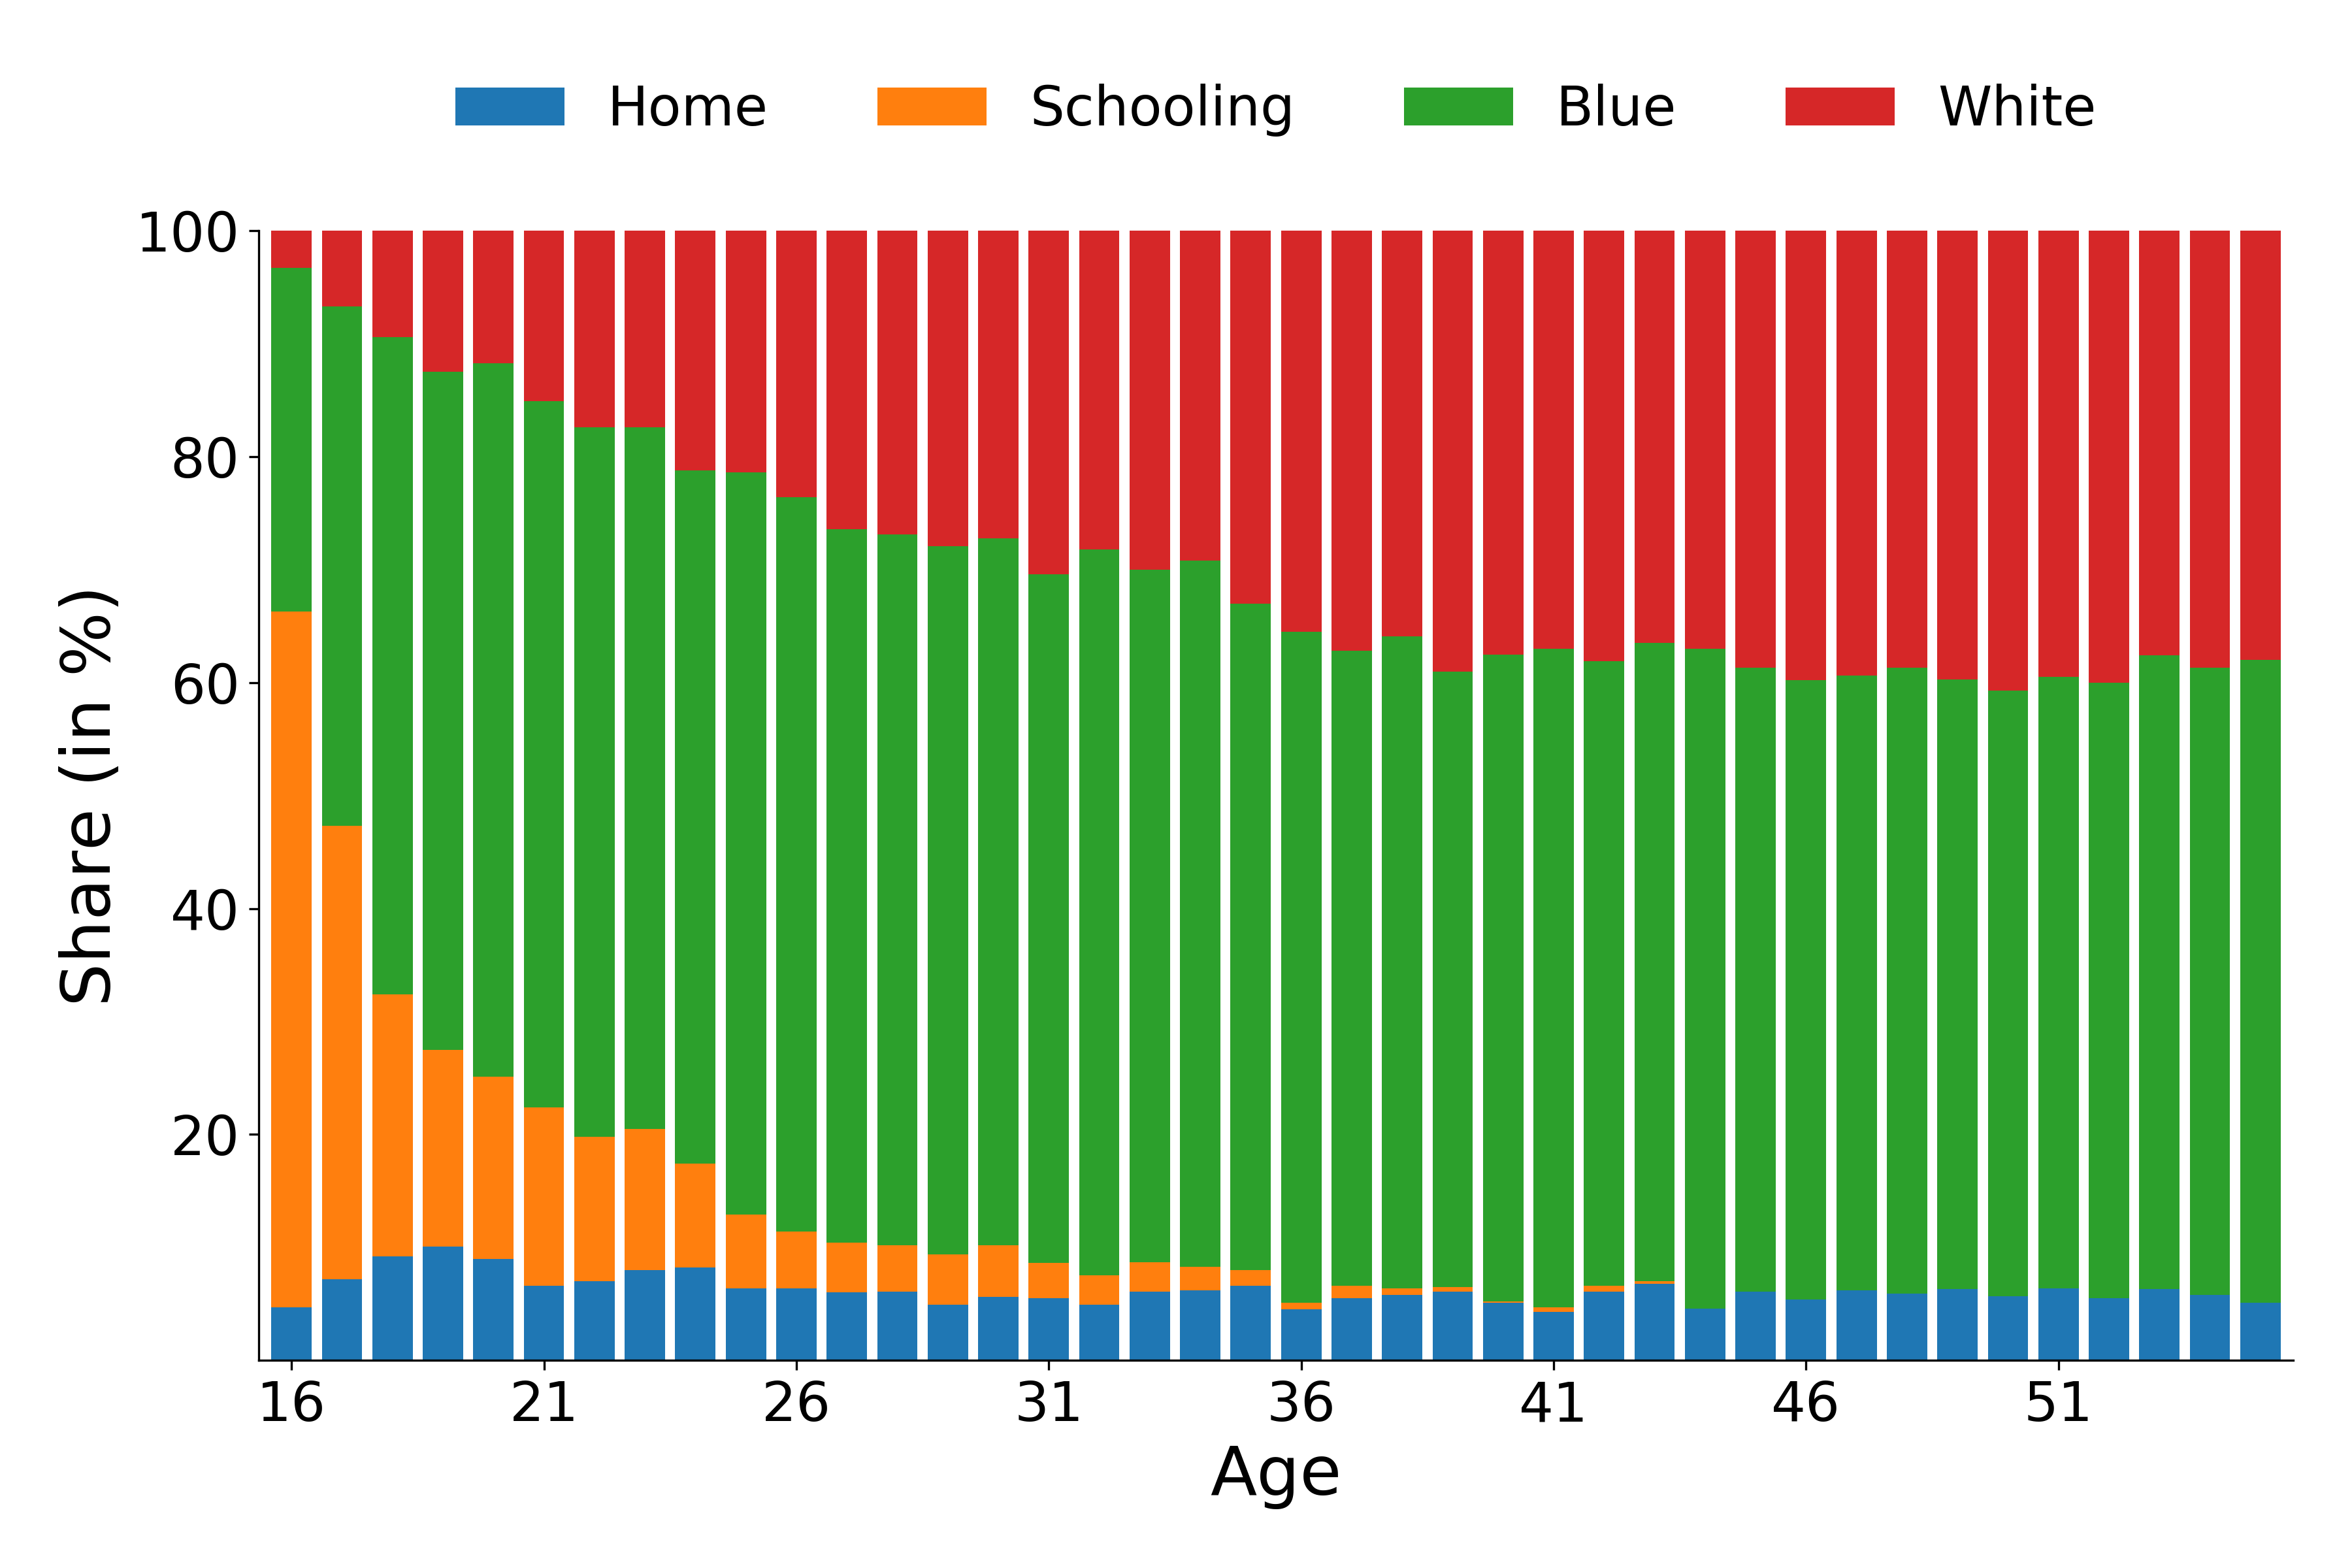
\includegraphics{fig-observed-choices}}
\end{figure}\FloatBarrier

\noindent Overall, the level of average final schooling is slightly above a high school degree with 12.6 years. Individuals incur the immediate costs of their schooling investments in the form of tuition and foregone earnings right at the beginning of their life cycle. Doing so allows them to get the most out of their increased wages in the future.

\paragraph{Economic mechanisms and policy evaluation} Figure \ref{Economic mechanism and policy forecast} illustrates the ability of structural economic models to quantify the impact of economic mechanisms and to forecast the effect of public policies. For both cases, we are interested in the effect on average final schooling. On the left, we vary the discount factor $\delta$ between $0.945$ and $0.955$ while we reduce $\beta_1$ by the size of a tuition subsidy of up to \$1.500.

\begin{figure}[h!]\centering
\caption{Economic mechanism and policy forecast}\label{Economic mechanism and policy forecast}
\subfloat[Time preference]{\scalebox{0.25}{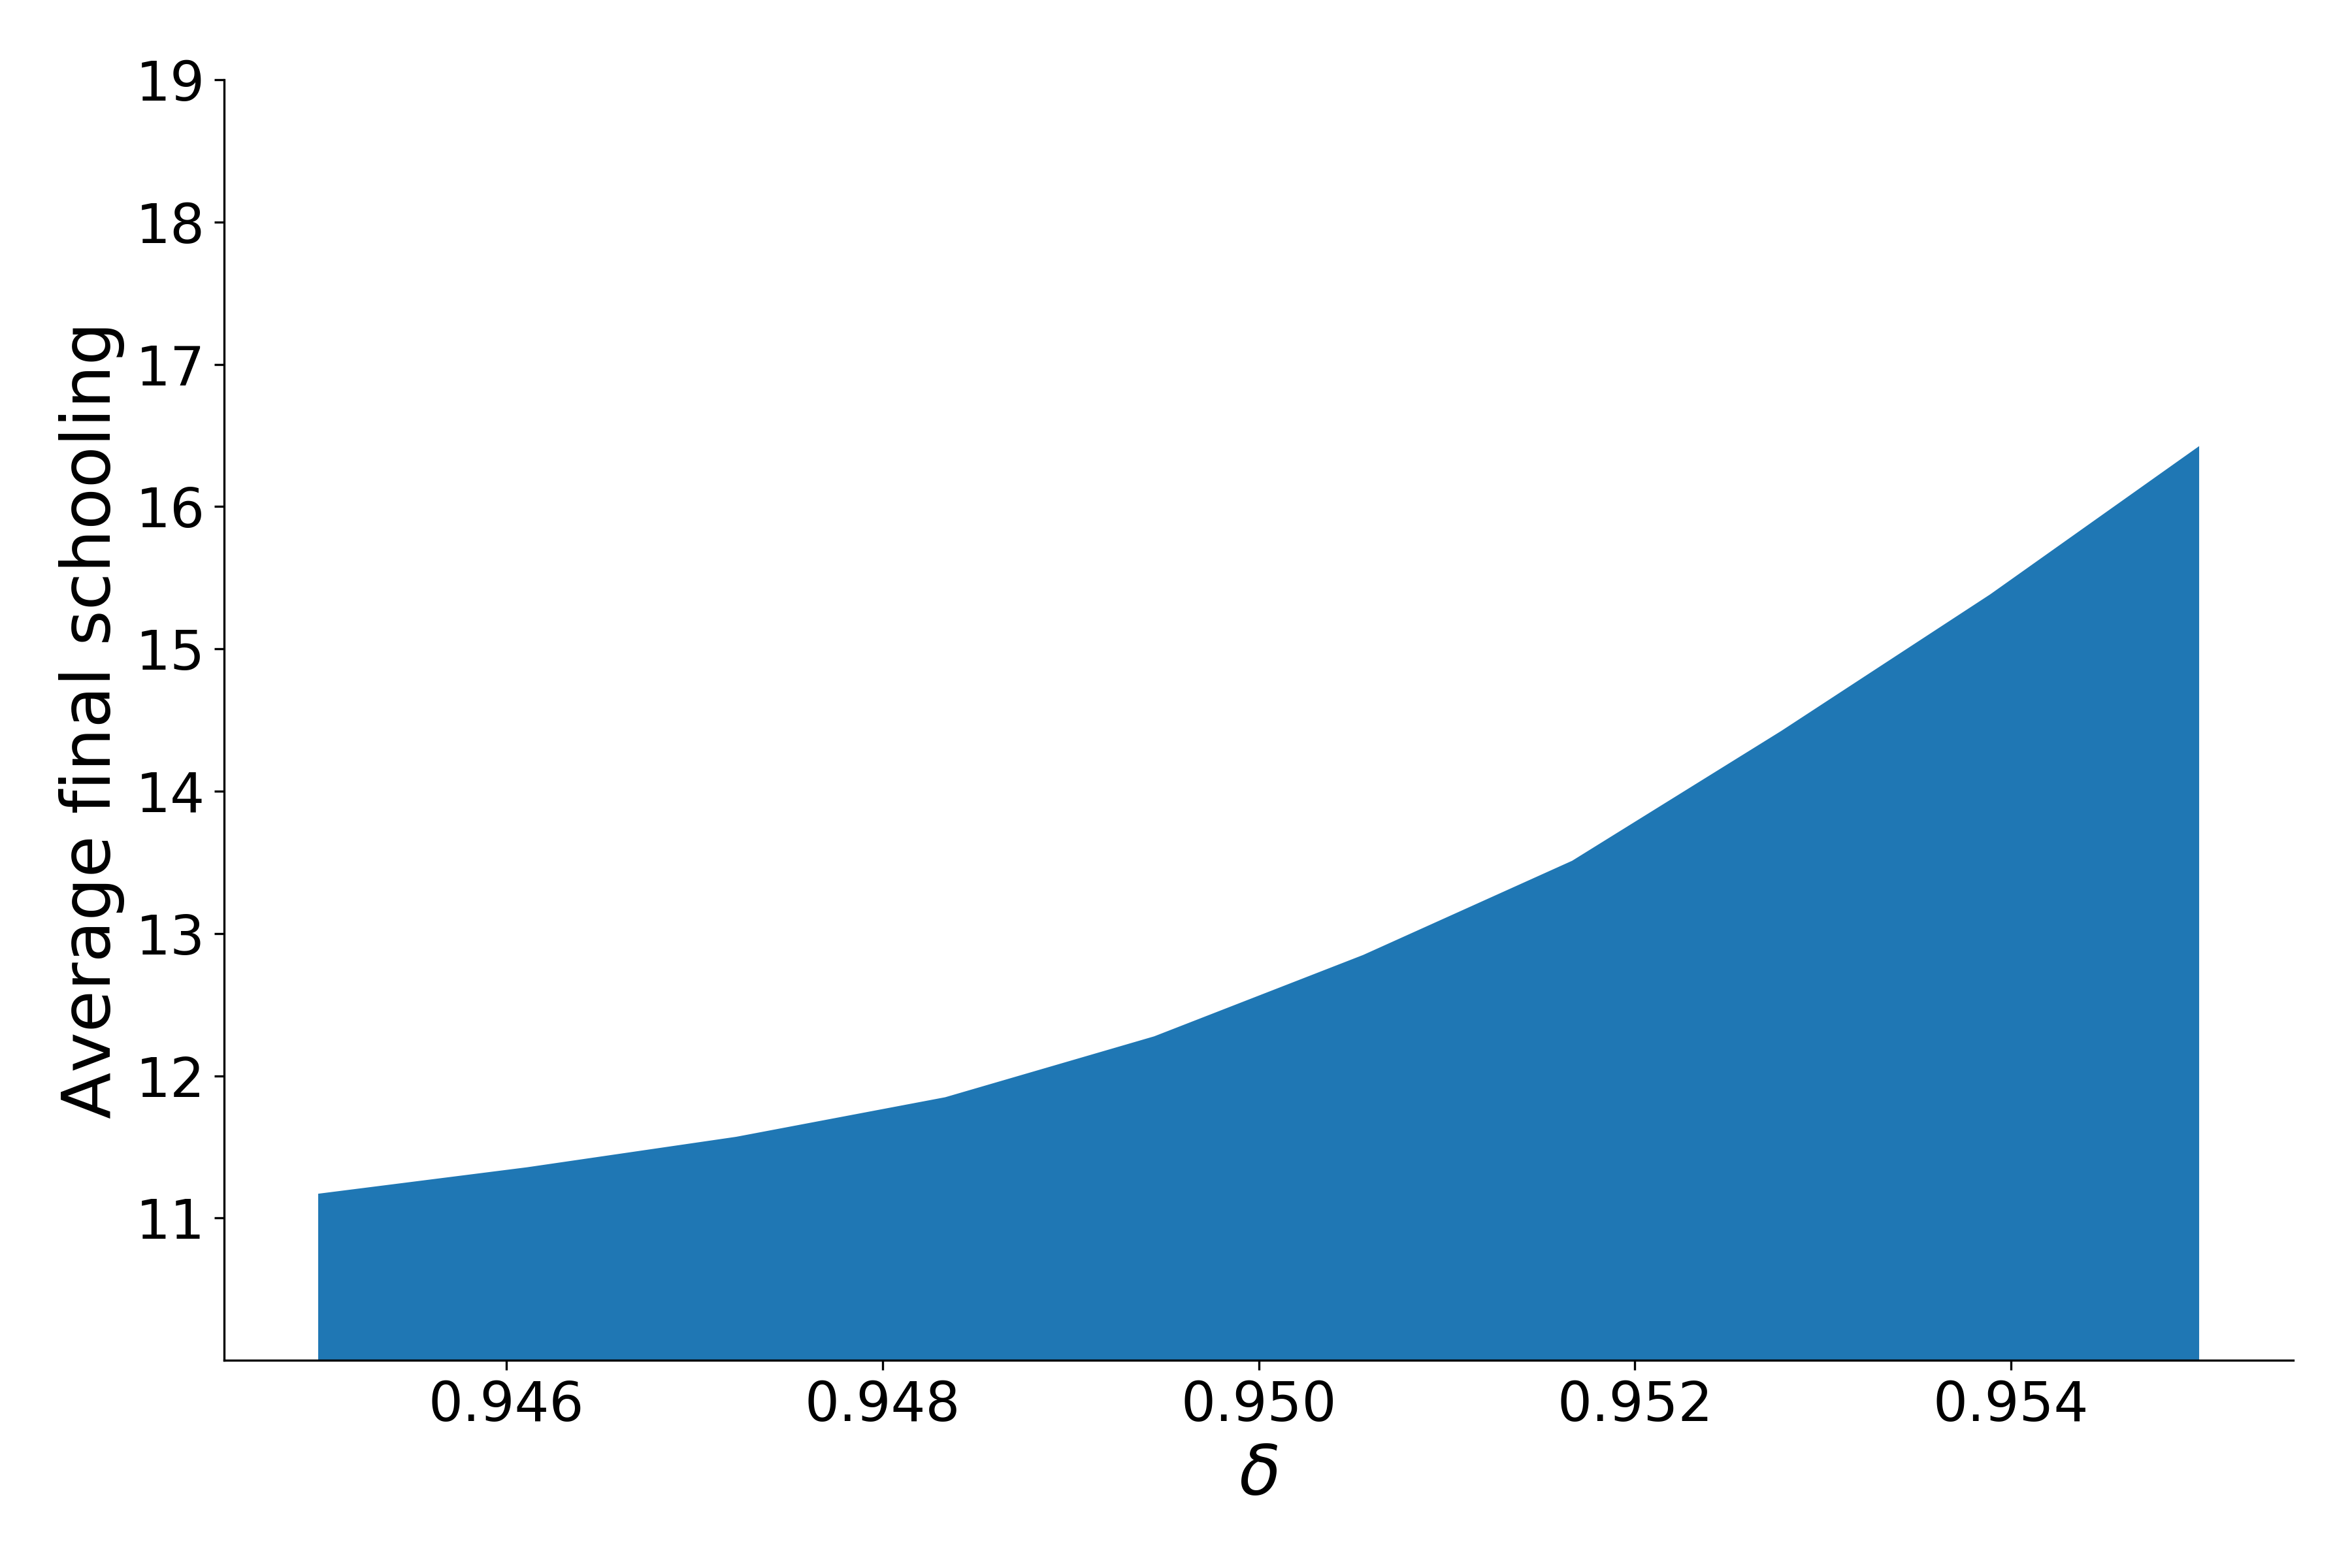
\includegraphics{fig-economic-mechanisms}}}\hspace{0.3cm}
\subfloat[Tuition subsidy]{\scalebox{0.25}{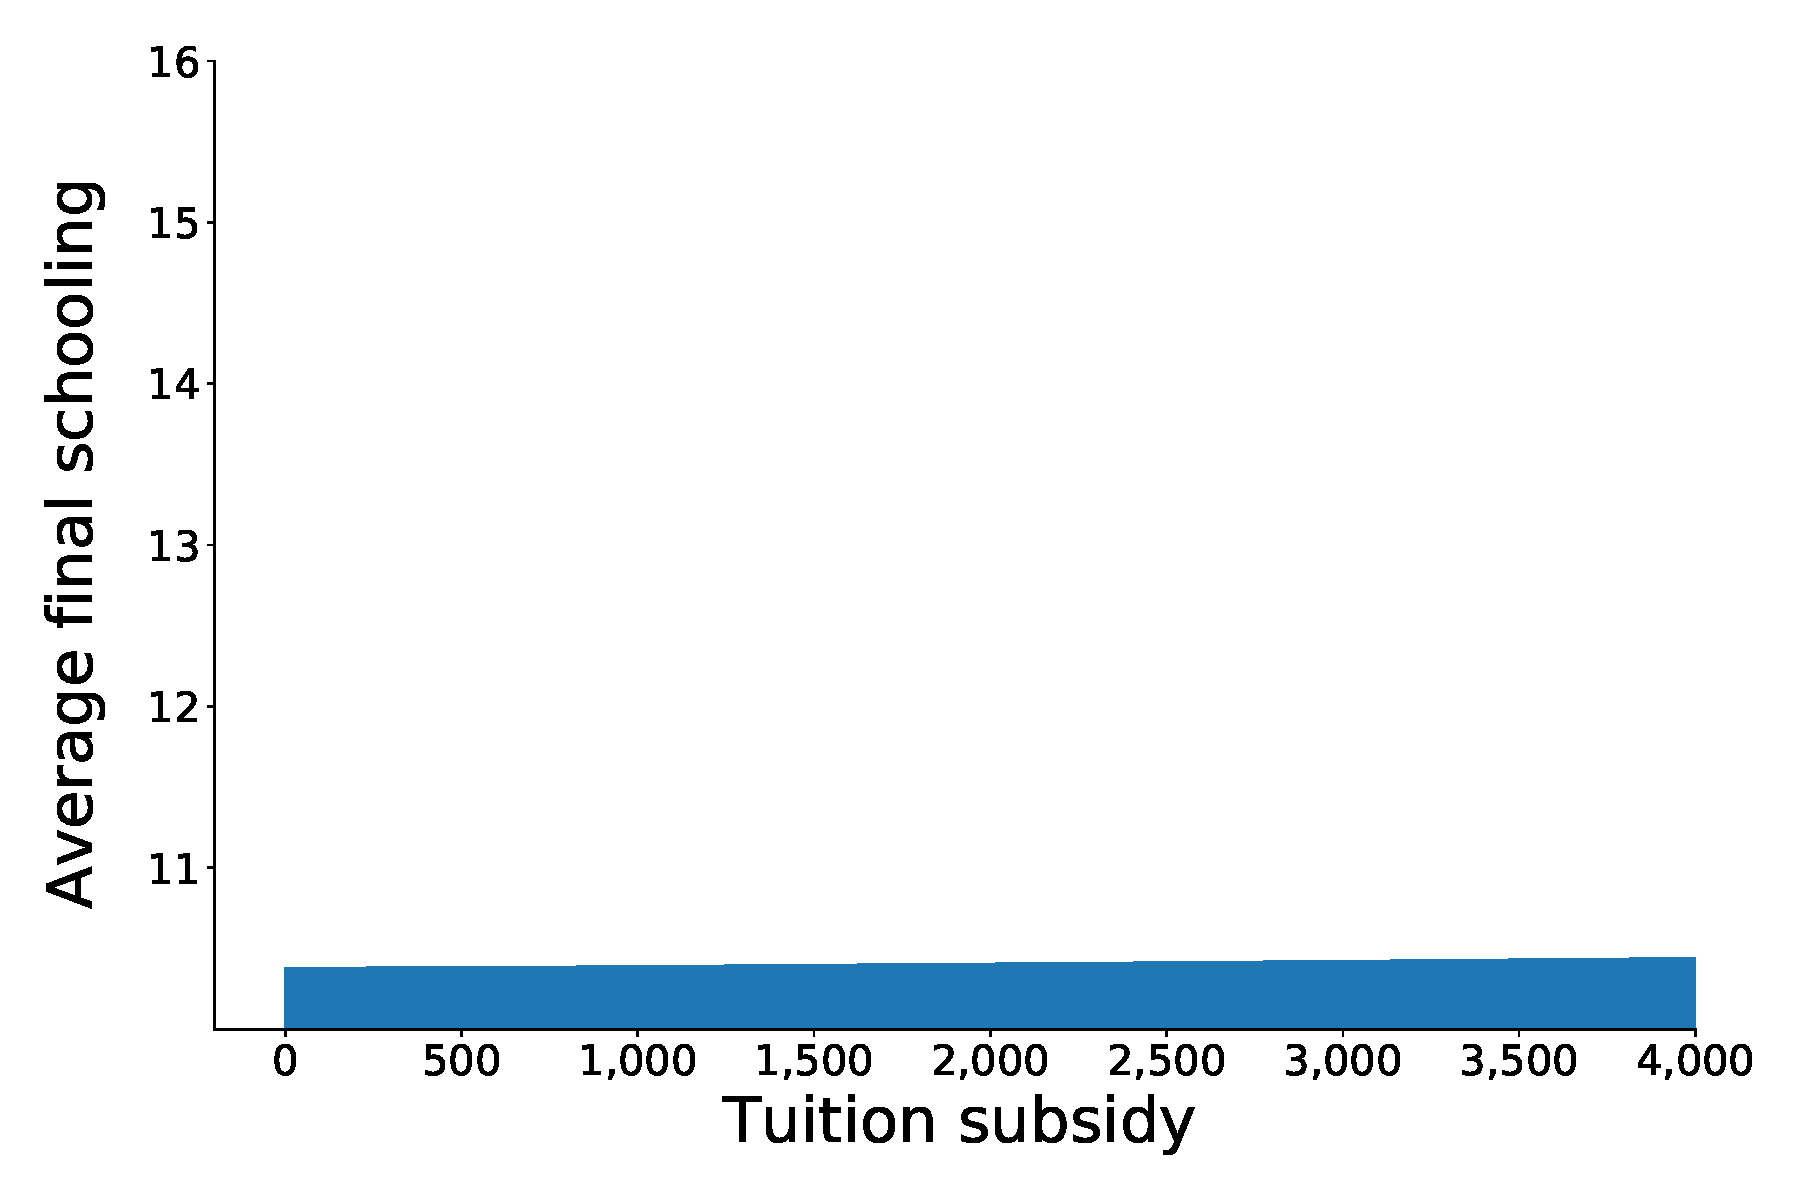
\includegraphics{fig-policy-forecast}}}
\end{figure}\FloatBarrier

\noindent Increases in the discount factor and the tuition subsidy both result in increased levels of average final schooling. However, they do so very different reasons. While individuals put more emphasis on the future benefits of their schooling investment in the former, they react to a reduction in its immediate cost in the latter.
%-------------------------------------------------------------------------------
\subsection{\texttt{respy}}
%-------------------------------------------------------------------------------
Our research group is actively developing the \verb+respy+ package, which allows for the flexible specification, simulation, and estimation of the typical EKW models. Instructions on how to use the package, obtain the source code, replicate several seminal papers, and details on the numerical methods are all available in its online documentation at \url{https://respy.readthedocs.io}.

\paragraph{Workflow illustration} Figure \ref{Workflow example} illustrates the typical workflow with the \verb+respy+ package.\footnote{The complete set of replication codes for the material included in this handout is available at \url{http://bit.ly/ekw-handout-replication}.} The model is specified in the parameters and options specification.

\begin{figure}[ht!]\centering
\caption{Workflow example}\label{Workflow example}
\lstset{language=python, morekeywords={as}, ndkeywords={=}, ndkeywordstyle=\color{blue}, keywordstyle=\color{red}, commentstyle=\color{darkgrey}, emph={get_example_model, get_crit_func, get_simulate_func}, emphstyle=\color{violet}, basicstyle=\footnotesize, frame=lines}
\begin{lstlisting}
import respy as rp

params, options, _ = rp.get_example_model("kw_94_one")
simulate = rp.get_simulate_func(params, options)
df = simulate(params)

\end{lstlisting}
\end{figure}


%!TEX root = ../main.tex
%-------------------------------------------------------------------------------
\section{Pipeline}
%-------------------------------------------------------------------------------

\begin{figure}[b!]\centering
	%\lstset{language=python, morekeywords={as}, ndkeywords={=}, ndkeywordstyle=\color{black}, keywordstyle=\color{black}, commentstyle=\color{black}, emph={}, emphstyle=\color{violet}, basicstyle=\footnotesize\ttfamily, frame=lines,   showlines=true}
	% From slides:
	\lstset{basicstyle=\footnotesize\ttfamily, language=python, morekeywords={as}, ndkeywords={=}, ndkeywordstyle=\color{blue}, numbers=left, keywordstyle=\color{red}, commentstyle=\color{darkgrey}, emph={get_example_model, get_crit_func, get_simulate_func}, emphstyle=\color{violet}}
	\lstinputlisting{../material/workflow.py}
	\caption{Typical workflow}\label{Typical workflow}
\end{figure}%\FloatBarrier

We are actively developing an ensemble of research codes that provide an analysis pipeline for EKW models. Among them are \verb+respy+ and \verb+estimagic+. The former allows for the flexible specification and simulation of EKW models while the latter provides the means for their calibration. We briefly showcase the typical workflow of using both packages in our research.


\autoref{Typical workflow} illustrates a typical workflow. Initially, the user provides the empirical data, the parameterization of the model, and other options to \verb+respy+. All together define the structure of the model, and we can construct the functionality for the simulation of data and the evaluation of the criterion function. \verb+estimagic+ allows calibrating the model to the empirical data. The results from the calibration steps are used to, for example, analyze the economic mechanisms underlying the observed behaviors.

\autoref{Model specification} shows the model specification files for \citet{Keane.1997}. The file on the left sets the parameter values for the utility functions and the distribution of the unobservable state variables. On the right, we provide details on the construction of the observed state variables and numerous tuning parameters for the numerical solution of the model.

\autoref{Dashboard} depicts the dashboard provided by \verb+estimagic+ to monitor the progress and parameter values of the calibration in real-time. This allows us to detect problems during calibration right away and facilitates the debugging process.

\begin{figure}[b!]\centering
	\subfloat[Parameterization]{\scalebox{0.39}{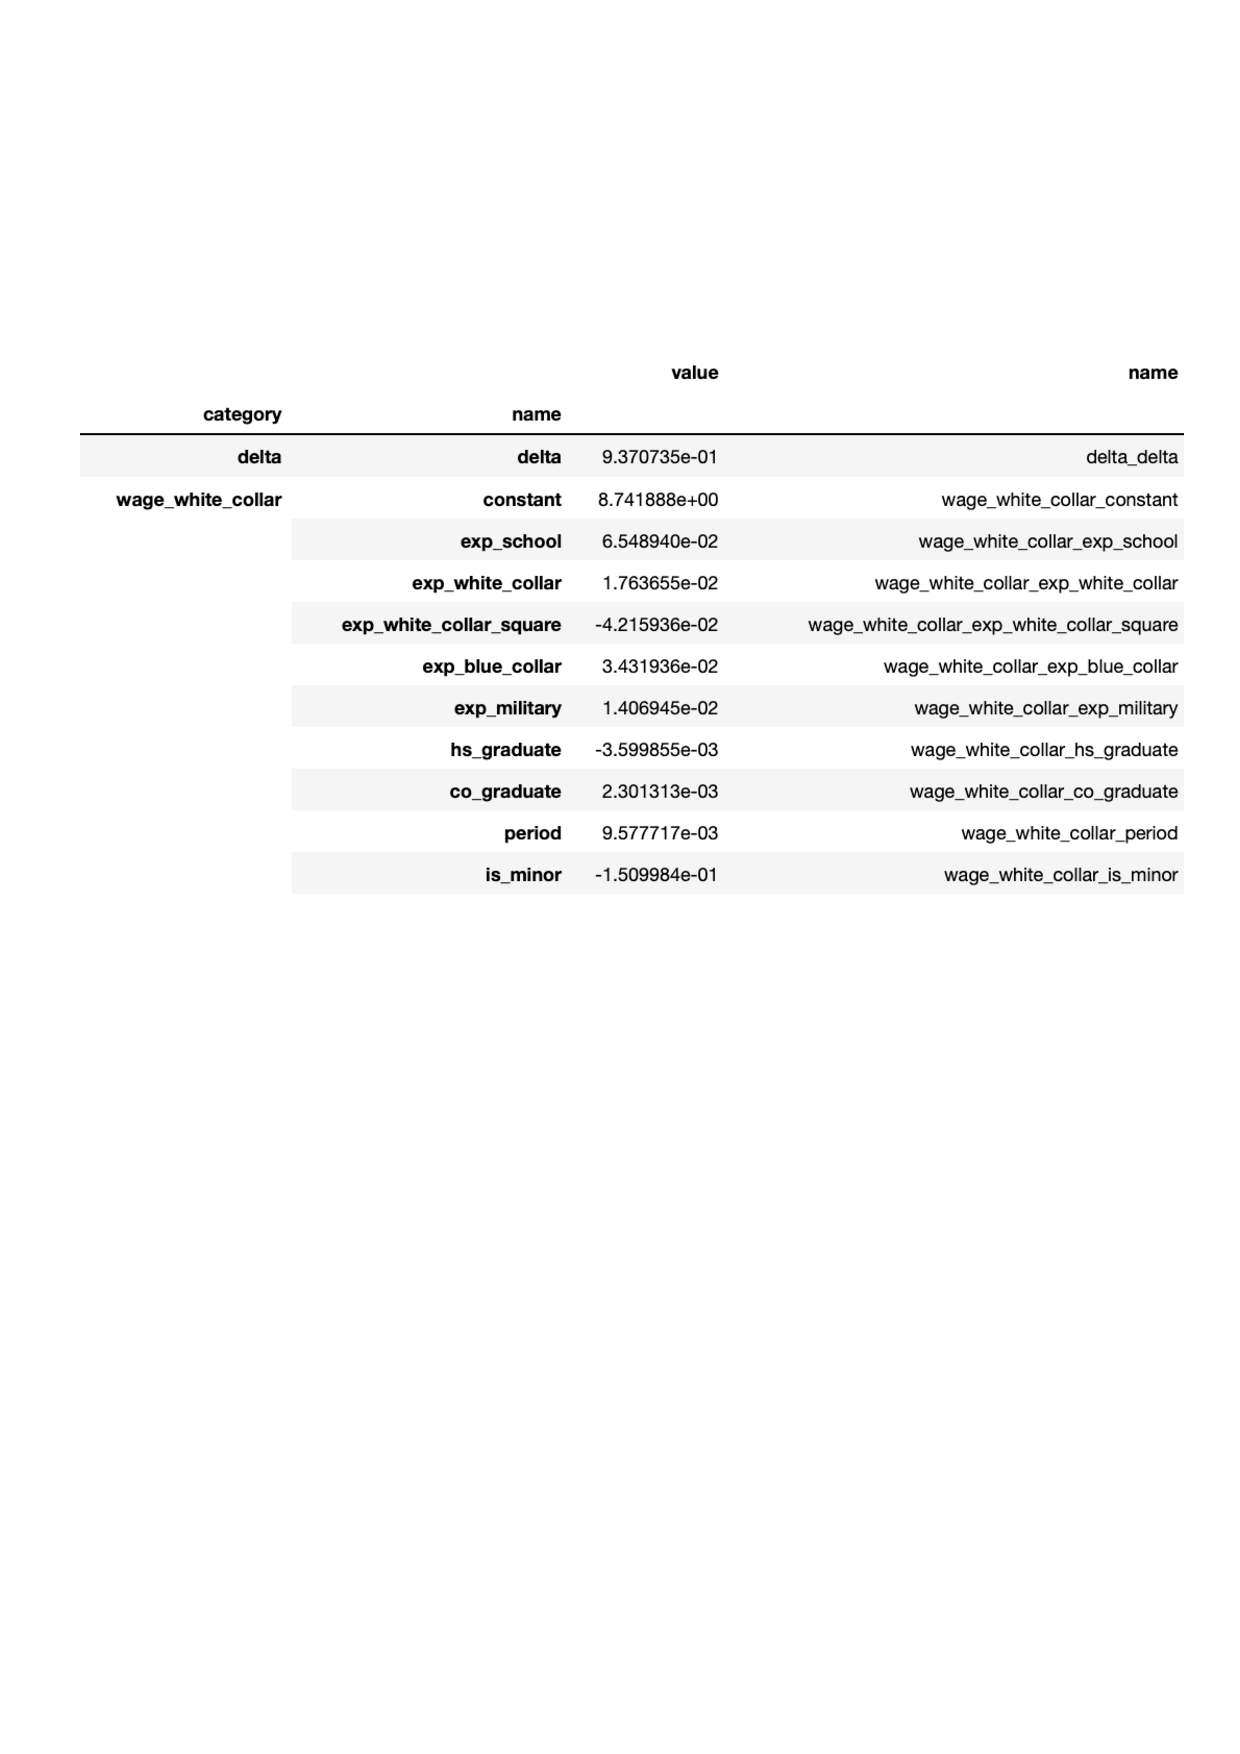
\includegraphics{crop-params.pdf}}}\hspace{0.3cm}
	\subfloat[Options]{\scalebox{0.39}{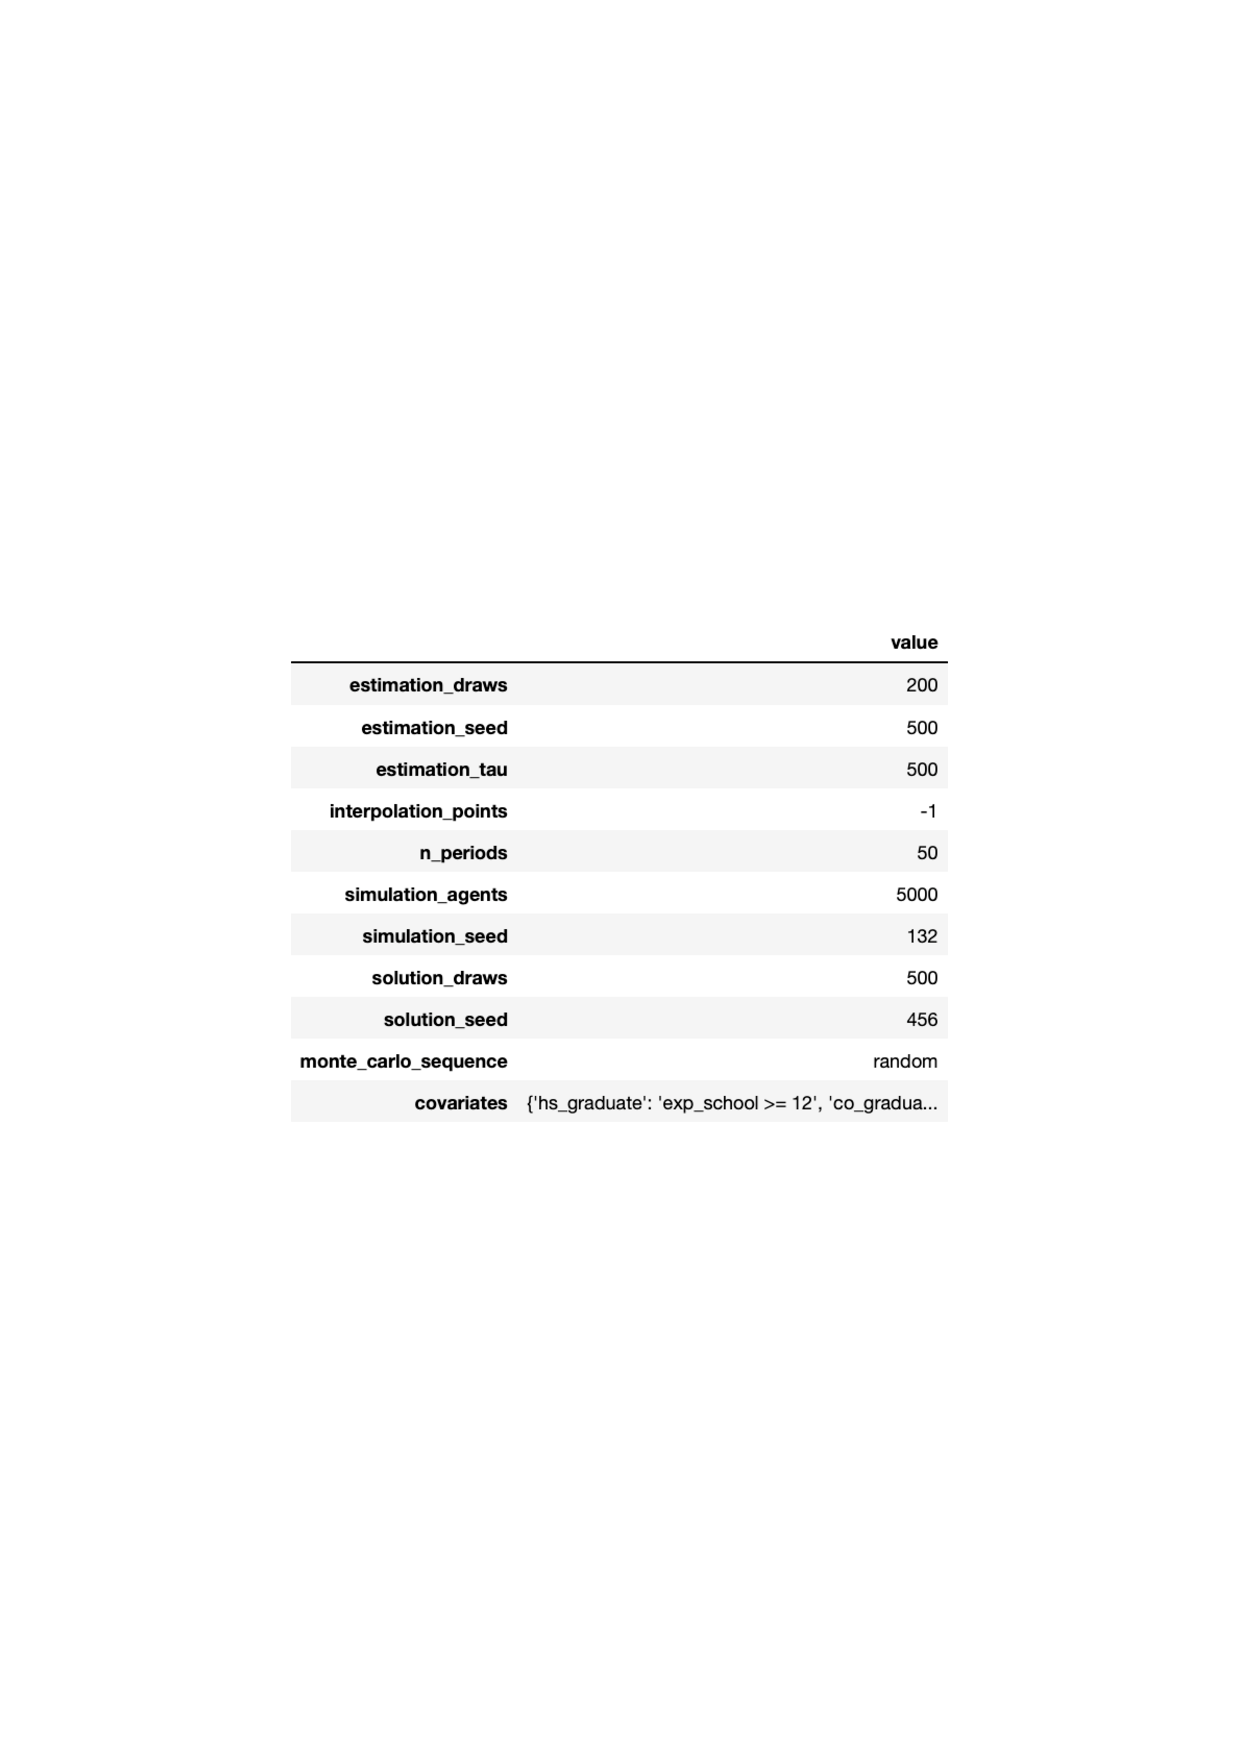
\includegraphics{crop-options.pdf}}}
	\caption{Model specification}\label{Model specification}
\end{figure}%\FloatBarrier

\begin{figure}[b!]\centering
\caption{Dashboard}\label{Dashboard}
\scalebox{0.40}{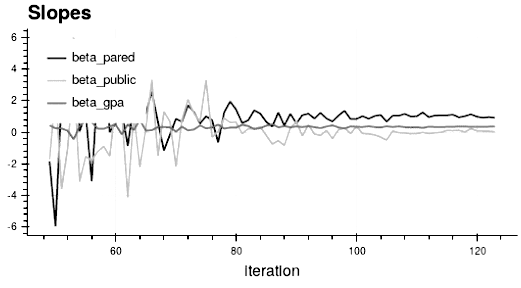
\includegraphics{crop-dashboard-black-white}}
\end{figure}%\FloatBarrier

We adopt a modern software engineering workflow in the development of both packages and tutorials, source code, testing harness, as well as implementation details are available in their respective online documentations at \url{https://respy.rtfd.io} and \url{https://estimagic.rtfd.io}.


% !TEX root = ../main.tex
\begin{frame}\begin{center}
\LARGE\textbf{Improvements}
\end{center}\end{frame}
%-------------------------------------------------------------------------------
%-------------------------------------------------------------------------------
\begin{frame}

\textbf{Improvements}\vspace{0.5cm}
\begin{itemize}\setlength\itemsep{1em}
\item Numerical integration \img{crop-active.png}
\item Global optimization \img{crop-active.png}
\item Function approximation  \img{crop-concept.png}
\item High-performance computing  \img{crop-concept.png}
\end{itemize}
\end{frame}


\clearpage

\begin{refcontext}[sorting=nyt]  % Sort BIBLIOGRAPHY by alphabet (while CITATIONS are sorted by year)
	\printbibliography[heading=bibintoc]
\end{refcontext}

\clearpage

\begin{appendices}
\setcounter{page}{1}
\renewcommand{\thepage}{\thesection-\arabic{page}}

\FloatBarrier% !TEX root = ../main.tex
%-------------------------------------------------------------------------------
\section{Computational implementation}\label{Computational implementation}
%-------------------------------------------------------------------------------
We use the same computational implementation as in \citet{Keane.1997}. We outline the immediate utility functions for each of the five alternatives. We first focus on their common overall structure and then present their parameterization. Throughout we provide the economic motivation for their specification.\\

\noindent We follow individuals over their working life from young adulthood at age 16 to retirement at age 65. The decision period $t = 16, \dots, 65$  is a school year and individuals decide $a\in\mathcal{A}$ whether to work in a blue-collar or white-collar occupation ($a = 1, 2$), to serve in the military $(a = 3)$, to attend school $(a = 4)$, or to stay at home $(a = 5)$.\\

\noindent Individuals are initially heterogeneous. They differ with respect to their initial level of completed schooling $h_{16}$ and have one of four different $\mathcal{J} = \{1, \hdots, 4\}$ alternative-specific skill endowments $\bm{e} = \left(e_{j,a}\right)_{\mathcal{J} \times \mathcal{A}}$.\\

\noindent The immediate utility $u_a(\cdot)$ of each alternative consists of a non-pecuniary utility $\zeta_a(\cdot)$ and, at least for the working alternatives, an additional wage component $w_a(\cdot)$. Both depend on the level of human capital as measured by their occupation-specific work experience $\bm{k_t} = \left(k_{a,t}\right)_{a\in\{1, 2, 3\}}$, years of completed schooling $h_t$, and alternative-specific skill endowment $\bm{e}$. The immediate utility functions are influenced by last-period choices $a_{t -1}$ and alternative-specific productivity shocks $\bm{\epsilon_t} = \left(\epsilon_{a,t}\right)_{a\in\mathcal{A}}$ as well. Their general form is given by:
%
\begin{align*}
u_a(\cdot) =
\begin{cases}
    \zeta_a(\bm{k_t}, h_t, t, a_{t -1})  + w_a(\bm{k_t}, h_t, t, a_{t -1}, e_{j, a}, \epsilon_{a,t})                & \text{if}\, a \in \{1, 2, 3\}  \\
    \zeta_a(\bm{k_t}, h_t, t, a_{t-1}, e_{j,a}, \epsilon_{a,t})                                                  &  \text{if}\, a \in \{4, 5\}.
\end{cases}
\end{align*}
%
Work experience $\bm{k_t}$  and years of completed schooling $h_t$ evolve deterministically.
%
\begin{align*}
k_{a,t+1} = k_{a,t} + \ind[a_t = a]  &\qquad \text{if}\, a \in \{1, 2, 3\} \\
h_{t + 1\phantom{,a}} = h_{t\phantom{,a}} +   \ind[a_t = 4]  &\qquad
\end{align*}
%
\noindent The productivity shocks are uncorrelated across time and follow a multivariate normal distribution with mean $\bm{0}$ and covariance matrix $\bm{\Sigma}$. Given the structure of the utility functions and the distribution of the shocks, the state at time $t$ is $s_t = \{\bm{k_t}, h_t, t, a_{t -1}, \bm{e},\bm{\epsilon_t}\}$.\\

\noindent Empirical and theoretical research from specialized disciplines within economics informs the exact specification of $u_a(\cdot)$. We now discuss each of its components in detail.
%-------------------------------------------------------------------------------
\subsection{Non-pecuniary utility}
%-------------------------------------------------------------------------------
We present the parameterization of the non-pecuniary utility for all five alternatives.
%-------------------------------------------------------------------------------
\subsubsection*{Blue-collar}
%-------------------------------------------------------------------------------
\noindent Equation (\ref{eq:NonWageBLueCollar}) shows the parameterization of the non-pecuniary utility from working in a blue-collar occupation.
%
\begin{align}\label{eq:NonWageBLueCollar}
\zeta_{1}(\bm{k_t}, h_t, a_{t-1})  = \alpha_1  &+ c_{1,1} \cdot \ind[a_{t-1} \neq 1] + c_{1,2} \cdot \ind[k_{1,t} = 0] \\ \nonumber
                            & + \vartheta_1 \cdot \ind[h_t \geq 12] + \vartheta_2 \cdot \ind[h_t \geq 16] + \vartheta_3 \cdot \ind[k_{3,t} = 1]
\end{align}
%
A constant $\alpha_1$ captures the net monetary-equivalent of on the job amenities. The non-pecuniary utility includes mobility and search costs $c_{1,1}$, which are higher for individuals who never worked in a blue-collar occupation before $c_{1,2}$. The non-pecuniary utilities capture returns from a high school $\vartheta_1$ and a college $\vartheta_2$ degree. Additionally, there is a detrimental effect of leaving the military early after one year $\vartheta_3$.
%-------------------------------------------------------------------------------
\subsubsection*{White-collar}
%-------------------------------------------------------------------------------
The non-pecuniary utility from working in a white-collar occupation is specified analogously. Equation (\ref{eq:UtilityWhiteCollar}) shows its parameterization.
%
\begin{align}\label{eq:UtilityWhiteCollar}
\zeta_{2}( \bm{k_t}, h_t, a_{t-1} ) = \,\alpha_2 & + c_{2,1} \cdot \ind[a_{t-1} \neq 2] + c_{2,2} \cdot \ind[k_{2,t} = 0]\\\nonumber
                            & + \vartheta_1 \cdot \ind[h_t \geq 12] + \vartheta_2 \cdot \ind[h_t \geq 16] + \vartheta_3 \cdot \ind[k_{3,t} = 1]
\end{align}
%-------------------------------------------------------------------------------
\subsubsection*{Military}
%-------------------------------------------------------------------------------
\noindent Equation (\ref{eq:UtilityMilitary}) shows the parameterization of the non-pecuniary utility from working in the military.
%
\begin{align}\label{eq:UtilityMilitary}
\zeta_{3}( k_{3.t}, h_t)  = \,& c_{3,2} \cdot \ind[k_{3,t} = 0]+ \vartheta_1 \cdot \ind[h_t \geq 12] + \vartheta_2 \cdot \ind[h_t \geq 16]
\end{align}
%
Search costs $c_{3, 1} = 0$ are absent but there is a mobility cost if an individual has never served in the military before $c_{3,2}$. Individuals still experience a non-pecuniary utility from finishing high-school $\vartheta_1$ and college $\vartheta_2$.
%-------------------------------------------------------------------------------
\subsubsection*{School}
%-------------------------------------------------------------------------------
Equation (\ref{eq:UtilitySchooling}) shows the parameterization of the non-pecuniary utility from schooling.
%
\begin{align}\label{eq:UtilitySchooling}
	\zeta_4(k_{3,t}, h_t, t, a_{t-1}, e_{j,4}, \epsilon_{4,t})  = e_{j,4} & + \beta_{tc_1} \cdot \ind[h_t \geq 12] + \beta_{tc_2} \cdot \ind[h_t \geq 16]   \\\nonumber
    							  & + \beta_{rc_1} \cdot \ind[a_{t-1} \neq 4, h_t < 12] + \beta_{rc_2} \cdot \ind[a_{t-1} \neq 4, h_t \geq 12] \\\nonumber
    							  & + \gamma_{4,4} \cdot t + \gamma_{4,5} \cdot \ind[t < 18] 																					  \\\nonumber
     							  & + \vartheta_1 \cdot \ind[h_t \geq 12] + \vartheta_2 \cdot \ind[h_t \geq 16] + \vartheta_3 \cdot \ind[k_{3,t} = 1]\\\nonumber
      							& + \epsilon_{4,t}
\end{align}
%
There is a direct cost of attending school such as tuition for continuing education after high school $\beta_{tc_1}$ and college $\beta_{tc_2}$. The decision to leave school is reversible, but entails adjustment costs that differ by schooling category ($\beta_{rc_1}, \beta_{rc_2}$). Schooling is defined as time spent in school and not by formal credentials acquired. Once individuals reach a certain amount of schooling, they acquire a degree. There is no uncertainty about grade completion \citep{Altonji.1993} and no part-time enrollment. Individuals value the completion of high-school and graduate school ($\vartheta_1, \vartheta_2$).
%-------------------------------------------------------------------------------
\subsubsection*{Home}
%-------------------------------------------------------------------------------
Equation (\ref{eq:UtilityHome}) shows the parameterization of the non-pecuniary utility from staying at home.
%
\begin{align}\label{eq:UtilityHome}
	\zeta_5(k_{3,t}, h_t, t, e_{j,5}, \epsilon_{5,1}) =  e_{j,5} & + \gamma_{5,4} \cdot \ind[18 \leq t \leq 20] + \gamma_{5,5} \cdot \ind[t \geq 21] \\ \nonumber
    							   & +\vartheta_{1} \cdot \ind[h_t \geq 12] + \vartheta_{2} \cdot \ind[h_t \geq 16] +  \vartheta_3 \cdot \ind[k_{3,t} = 1]  \\ \nonumber
    							   & + \epsilon_{5,t}
\end{align}
%
Staying at home as a young adult $\gamma_{5, 4}$ is less stigmatic as doing so while already being an adult $\gamma_{5,5}$. Additionally, possessing a degree  $(\vartheta_1, \vartheta_2)$ or leaving the military prematurely $\vartheta_3$ influences the immediate utility.
%-------------------------------------------------------------------------------
\subsection{Wage component}
%-------------------------------------------------------------------------------
The wage component $w_{a}(\cdot)$ for the working alternatives is given by the product of the market-equilibrium rental price $r_{a}$ and an occupation-specific skill level $x_{a}(\cdot)$. The latter is determined by the overall level of human capital.
%
\begin{align*}
w_{a}(\cdot) = r_{a} \, x_{a}(\cdot)
\end{align*}
%
This specification leads to a standard logarithmic wage equation in which the constant term is the skill rental price $\ln(r_{a})$ and wages follow a log-normal distribution.\\

\noindent The occupation-specific skill level $x_{a}(\cdot)$ is determined by a skill production function, which includes a deterministic component $\Gamma_a(\cdot)$ and a multiplicative stochastic productivity shock $\epsilon_{a,t}$.
%
\begin{align}
    x_{a}(\bm{k_t}, h_t, t, a_{t-1}, e_{j, a}, \epsilon_{a,t}) & = \exp \big( \Gamma_{a}(\bm{k_t},  h_t, t, a_{t-1}, e_{j,a}) \cdot \epsilon_{a,t} \big) \nonumber
\end{align}
%-------------------------------------------------------------------------------
\subsubsection*{Blue-collar}
%-------------------------------------------------------------------------------
Equation (\ref{eq:SkillLevelBlueCollar}) shows the parameterization of the deterministic component of the skill production function.
%
\begin{align}\label{eq:SkillLevelBlueCollar}
    \Gamma_1(\bm{k_t}, h_t, t, a_{t-1}, e_{j, 1}) = e_{j,1} & + \beta_{1,1} \cdot h_t + \beta_{1, 2} \cdot \ind[h_t \geq 12] + \beta_{1,3} \cdot \ind[h_t\geq 16]\\ \nonumber
                                  & + \gamma_{1, 1} \cdot  k_{1,t} + \gamma_{1,2} \cdot  (k_{1,t})^2 + \gamma_{1,3} \cdot  \ind[k_{1,t} > 0] \\ \nonumber
                                & + \gamma_{1,4} \cdot  t + \gamma_{1,5} \cdot \ind[t < 18]\\ \nonumber
                                  & + \gamma_{1,6} \cdot \ind[a_{t-1} = 1] + \gamma_{1,7} \cdot  k_{2,t} + \gamma_{1,8} \cdot  k_{3,t} \nonumber
\end{align}
%
There are several notable features. The first part of the skill production function is motivated by \citet{Mincer.1958, Mincer.1974} and hence linear in years of completed schooling $\beta_{1,1}$, quadratic in experience ($\gamma_{1,1}, \gamma_{1,2}$), and separable between the two of them. There are so-called sheep-skin effects \citep{Hungerford.1987, Jaeger.1996} associated with completing a high school $\beta_{1,2}$ and graduate $\beta_{1,3}$ education that capture the impact of completing a degree beyond just the associated years of schooling. Also, there is a first-year blue-collar experience effect $\gamma_{1,3}$ while skills depreciate when not employed in a blue-collar occupation in the preceding period $\gamma_{1,6}$. Other work experience ($\gamma_{1,7}, \gamma_{1,8}$) is transferable.
%-------------------------------------------------------------------------------
\subsubsection*{White-collar}
%-------------------------------------------------------------------------------
The wage component from working in a white-collar occupation is specified analogously. Equation (\ref{eq:SkillLevelWhiteCollar}) shows the parameterization of the deterministic component of the skill production function.
%
\begin{align}\label{eq:SkillLevelWhiteCollar}
    \Gamma_2(\bm{k_t}, h_t, t, a_{t-1}, e_{j,2}) = e_{j,2} & + \beta_{2,1} \cdot h_t + \beta_{2, 2} \cdot \ind[h_t \geq 12] + \beta_{2,3} \cdot \ind[h_t\geq 16] \\\nonumber
    							 & + \gamma_{2, 1} \cdot  k_{2,t} + \gamma_{2,2} \cdot  (k_{2,t})^2 + \gamma_{2,3} \cdot  \ind[k_{2,t} > 0] \\\nonumber
                                   & + \gamma_{2,4} \cdot  t + \gamma_{2,5} \cdot \ind[t < 18] \\\nonumber
                                  & + \gamma_{2,6} \cdot  \ind[a_{t-1} = 2]  + \gamma_{2,7} \cdot  k_{1,t} + \gamma_{2,8} \cdot  k_{3,t}
\end{align}
%-------------------------------------------------------------------------------
\subsubsection*{Military}
%-------------------------------------------------------------------------------
Equation (\ref{eq:SkillLevelMilitary}) shows the parameterization of the deterministic component of the skill production function.
%
\begin{align}\label{eq:SkillLevelMilitary}
    \Gamma_3( k_{3,t}, h_t, t, e_{j,3}) = e_{j,3} & + \beta_{3,1} \cdot h_t \\\nonumber
	               \nonumber &+ \gamma_{3,1} \cdot  k_{3,t} + \gamma_{3,2} \cdot (k_{3,t})^2 + \gamma_{3,3} \cdot \ind[k_{3,t} > 0]\\\nonumber
									 & + \gamma_{3,4} \cdot t + \gamma_{3,5} \cdot \ind[t < 18]
\end{align}
%
Contrary to the civilian sector there are no sheep-skin effects from graduation ($\beta_{3,2} = \beta_{3,3}= 0$). The previous occupational choice has no influence ($\gamma_{3,6}= 0$) and any experience other than military is non-transferable ($\gamma_{3,7} = \gamma_{3,8} = 0$).

\begin{Remark} Our parameterization for the immediate utility of serving in the military differs from \citet{Keane.1997} as we remain unsure about their exact specification. The authors state in Footnote 31 (p.498) that the constant for the non-pecuniary utility $\alpha_{3,t}$ depends on age. However, we are unable to determine the precise nature of the relationship. Equation (C3) (p.521) also indicates no productivity shock $\epsilon_{a,t}$ in the wage component. Table 7 (p.500) reports such estimates.
\end{Remark}
%-------------------------------------------------------------------------------
\FloatBarrier\subsection{Overview parameters}
%-------------------------------------------------------------------------------

\begin{ThreePartTable}
% Information available at https://ftp.agdsn.de/pub/mirrors/latex/dante/macros/latex/contrib/threeparttablex/threeparttablex.pdf

\begin{TableNotes}
	\item \textbf{Note:} The listed parameters are represented as an overview. The per-period utilities for the alternatives do not necessarily include all of them.
\end{TableNotes}

\begin{longtable}{@{}cll@{}}
\caption{Overview of parameters in the \citet{Keane.1997} extended model.}
\label{tab:ModelParameters}

\setlength\extrarowheight{2.5pt}

% Settings longtable
\\
\toprule 
\textbf{Parameter}            &  &  \multicolumn{1}{l}{\textbf{Description}}              \\ \midrule 
\endfirsthead 

% Alternative 1 header for the beginning on next page
%\midrule
%Parameter            &  &  \multicolumn{1}{l}{Description}     \\ \midrule

% Alternative 2 header for the beginning on next page
\multicolumn{3}{c}{\tikz\draw [thick,dash dot] (0,0) -- (15,0);} \vspace{-5pt} \\
\multicolumn{3}{c}{continued from previous page} \vspace{-10pt} \\
\multicolumn{3}{c}{\tikz\draw [thick,dash dot] (0,0) -- (15,0);} \\
\endhead 

\multicolumn{3}{c}{\tikz\draw [thick,dash dot] (0,0) -- (15,0);} \vspace{-5pt} \\
\multicolumn{3}{c}{continued on next page } \vspace{-10pt} \\
\multicolumn{3}{c}{\tikz\draw [thick,dash dot] (0,0) -- (15,0);} \\
\endfoot

\bottomrule 
\insertTableNotes
\endlastfoot 

% Start table
\midrule
\multicolumn{3}{l}{Preference and type-specific parameters}																		 \\ \midrule 
$\delta$ 				&  & discount factor																			  \\
$e_{j, a}$			&  & initial endowment of type $j$ in alternative $a$ specific skills 	  \\ [7.5pt] \midrule 
\multicolumn{3}{l}{Common parameters per-period utility}												\\ \midrule 
$\alpha_a$           &  & return non-wage working conditions		   \\
$\vartheta_1$        &  & non-pecuniary premium of finishing high-school                 								    \\
$\vartheta_2$        &  & non-pecuniary premium finishing college															    \\
$\vartheta_3$        &  & non-pecuniary premium of leaving military early						  \\[7.5pt] \midrule 
\multicolumn{3}{l}{Schooling-related parameters}															   \\ \midrule
% Work
$\beta_{a,1}$        &  & return additional year of completed schooling 								\\
$\beta_{a,2}$        &  & skill premium high-school graduate										      \\
$\beta_{a,3}$        &  & skill premium college graduate													   	\\
% Military
% School
$\beta_{tc_1}$       &  & tuition cost high-school                      											\\
$\beta_{tc_2}$       &  & tuition cost college                          												\\
$\beta_{rc_1}$       &  & re-entry cost high-school                     										   \\
$\beta_{rc_2}$       &  & re-entry cost college                        												   \\
% Home
$\beta_{5,2}$        &  & skill premium high-school graduate            									\\
$\beta_{5,3}$        &  & skill premium college graduate                									     \\ [7.5pt] \midrule
\multicolumn{3}{l}{Experience-related parameters}           													 \\
\midrule 
$\gamma_{a,1}$       &  & return same-sector experience                 									 \\
$\gamma_{a,2}$       &  & return squared same-sector experience         								\\
$\gamma_{a,3}$       &  & premium having worked in sector before        							   \\
$\gamma_{a,4}$       &  & return age effect                             											     \\
$\gamma_{a,5}$       &  & return age effect being a minor               										\\
$\gamma_{a,6}$       &  & premium remaining in same sector              								   \\
$\gamma_{a,7}$       &  & return civilian cross-sector experience       								    \\
$\gamma_{a,8}$       &  & return non-civilian sector experience       										 \\
$\gamma_{3,1}$       &  & return same-sector experience                 									  \\
$\gamma_{3,2}$       &  & return squared same-sector experience    										 \\
$\gamma_{3,3}$       &  & premium having worked in sector before   										\\
$\gamma_{3,4}$       &  & return age effect                             												 \\
$\gamma_{3,5}$       &  & return age effect being a minor              	   										\\
$\gamma_{4,4}$       &  & return age effect                             												 \\
$\gamma_{4,5}$       &  & return age effect being a minor                  										\\
$\gamma_{5,4}$       &  & return age between 17 and 21                 	  									   \\
$\gamma_{5,5}$       &  & return age older than 20							   										\\[7.5pt] \midrule
\multicolumn{3}{l}{Mobility and search parameters}          													  \\ \midrule 
$c_{a,1}$            &  & premium switching to occupation $a$           									   \\
$c_{a,2}$            &  & premium for working first time in occupation $a$         										  \\
$c_{3,2}$            &  & premium for serving first time in military    										  \\[7.5pt] \midrule
\multicolumn{3}{l}{Error correlation}          													  									\\ \midrule 
$\sigma_{a,a}$	&	& standard deviation of shock in alternative $a$									\\
$\sigma_{i,j}$ &	& correlation between shocks of alternative $a = i$ and $a=j$ with $i \neq j$ \\

\end{longtable}
\end{ThreePartTable}



\clearpage
\setcounter{page}{1}
\FloatBarrier% !TEX root = ../main.tex
%-------------------------------------------------------------------------------
\section{Empirical data}\label{Empirical data}
%-------------------------------------------------------------------------------
We use the same data as in \citet{Keane.1997}. Please see \url{https://bit.ly/ekw-data} for details.

\subsection{Model fit}

We provide a full stack of comparisons between simulated and empirical data. We simulate a sample of 1,000 individuals using the calibrated model.



\begin{figure}[h]\centering
	\caption{Model fit}\label{Model fit appendix}
	\subfloat[White-collar]{\scalebox{0.19}{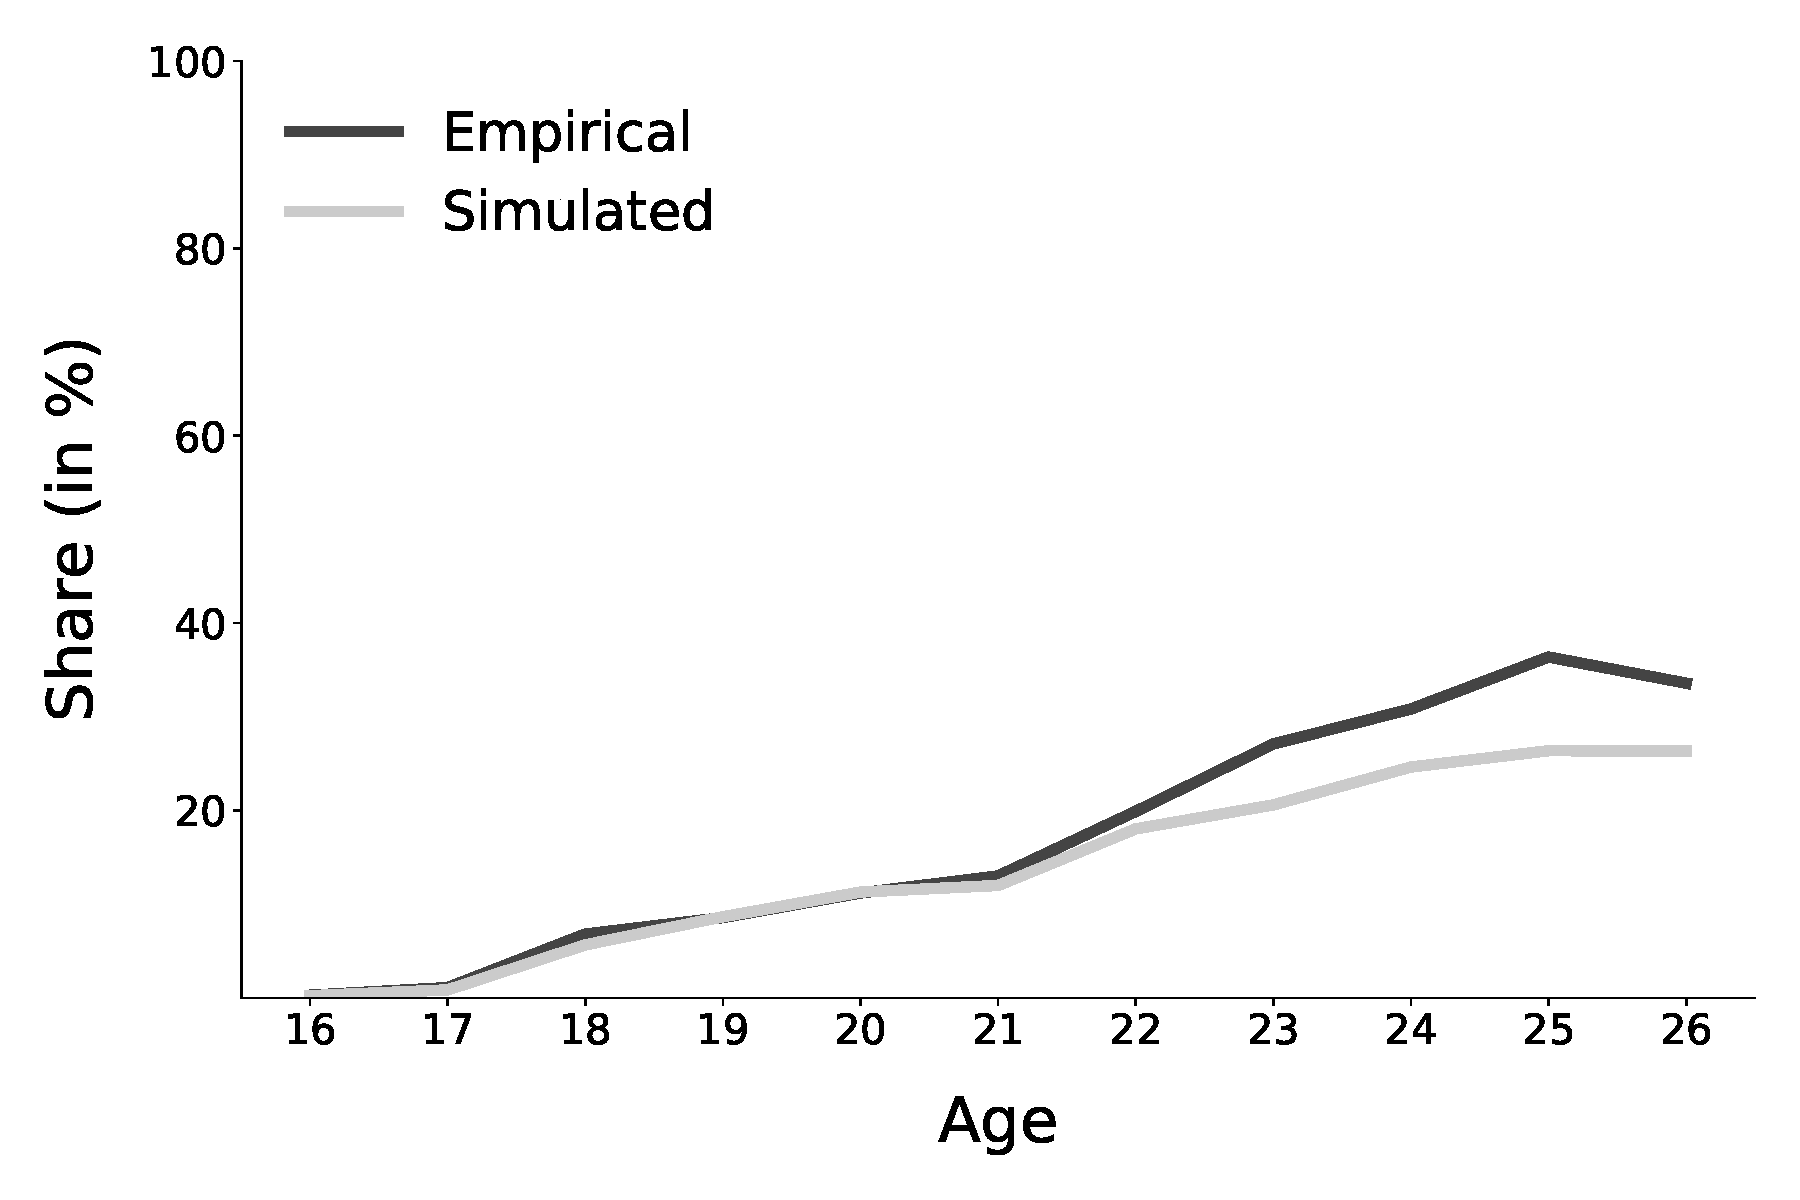
\includegraphics{fig-model-fit-choice-white-bw}}}\hspace{0.3cm}
	\subfloat[Military]{\scalebox{0.19}{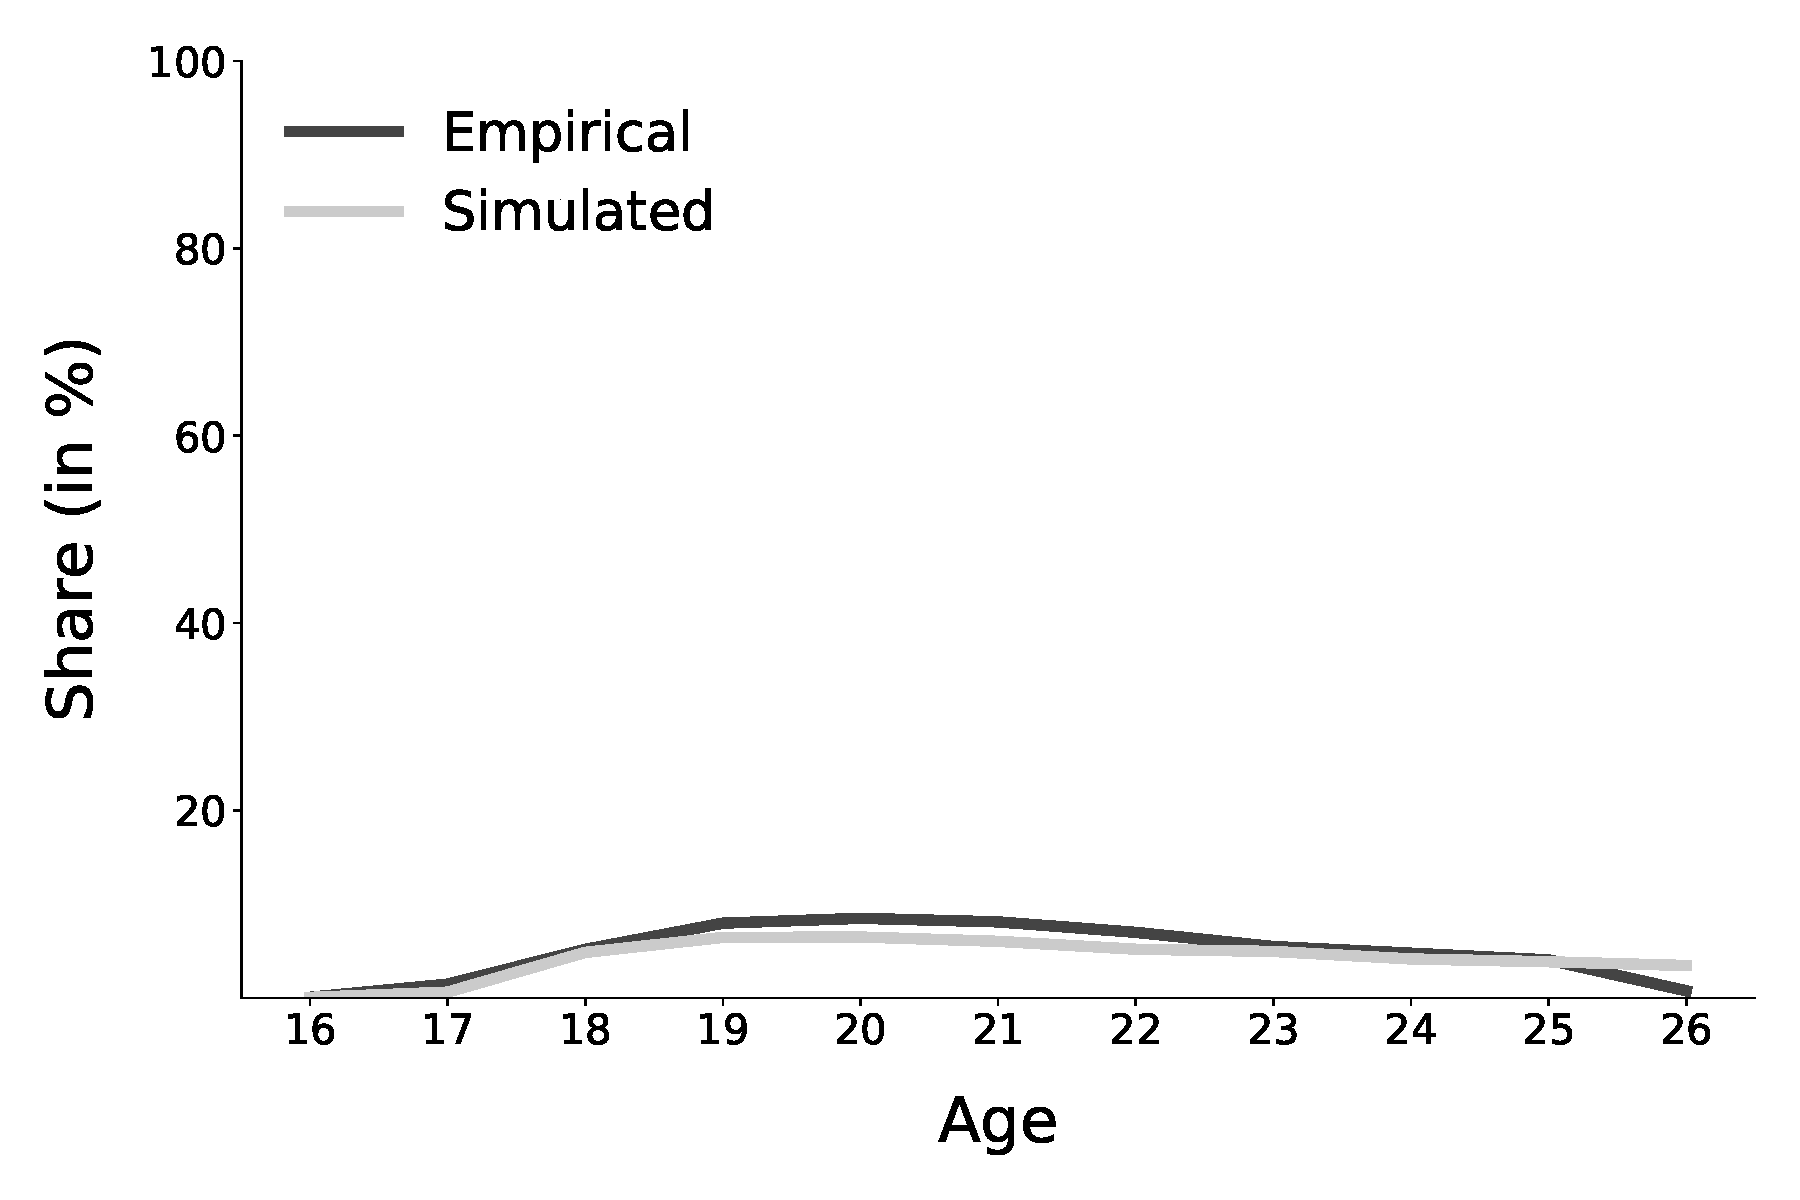
\includegraphics{fig-model-fit-choice-military-bw}}} \\
	\subfloat[School]{\scalebox{0.19}{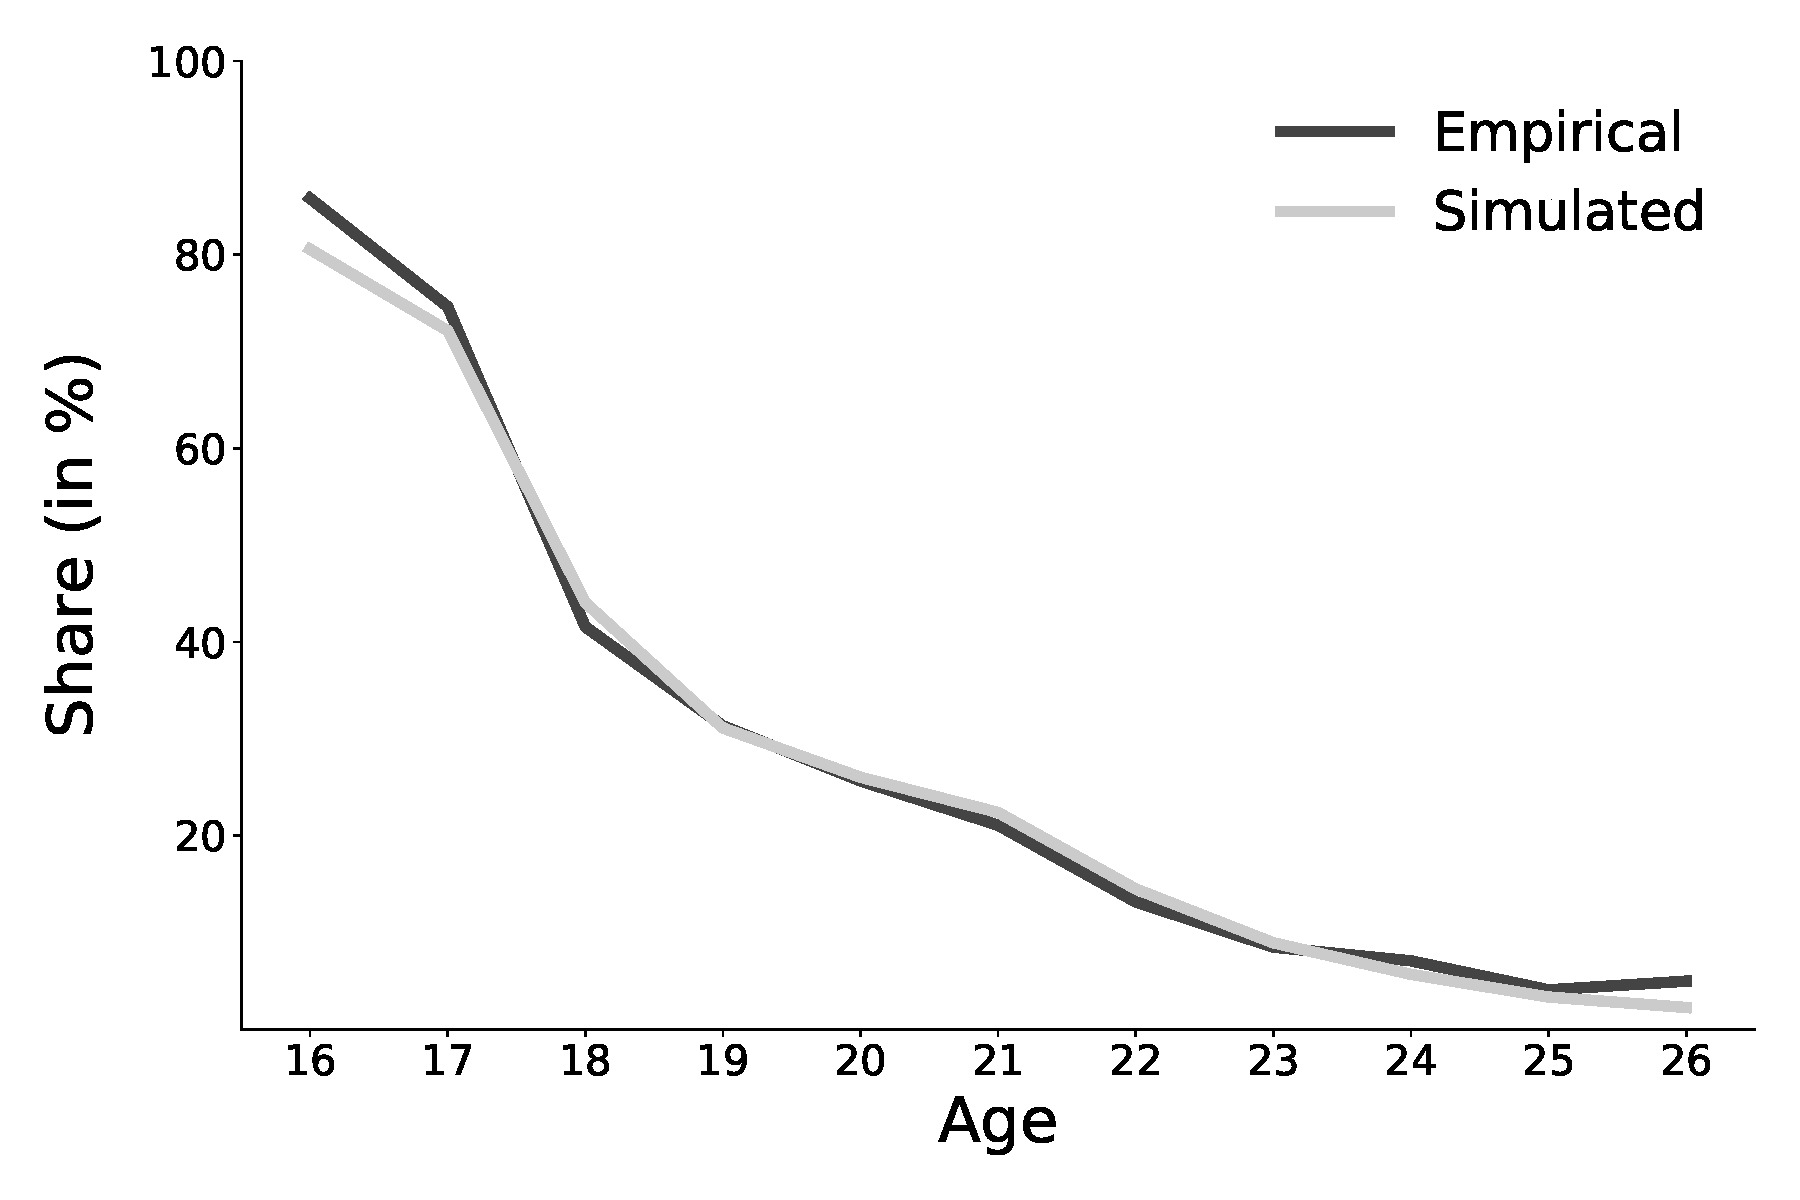
\includegraphics{fig-model-fit-choice-school-bw}}}\hspace{0.3cm}
	\subfloat[Home]{\scalebox{0.19}{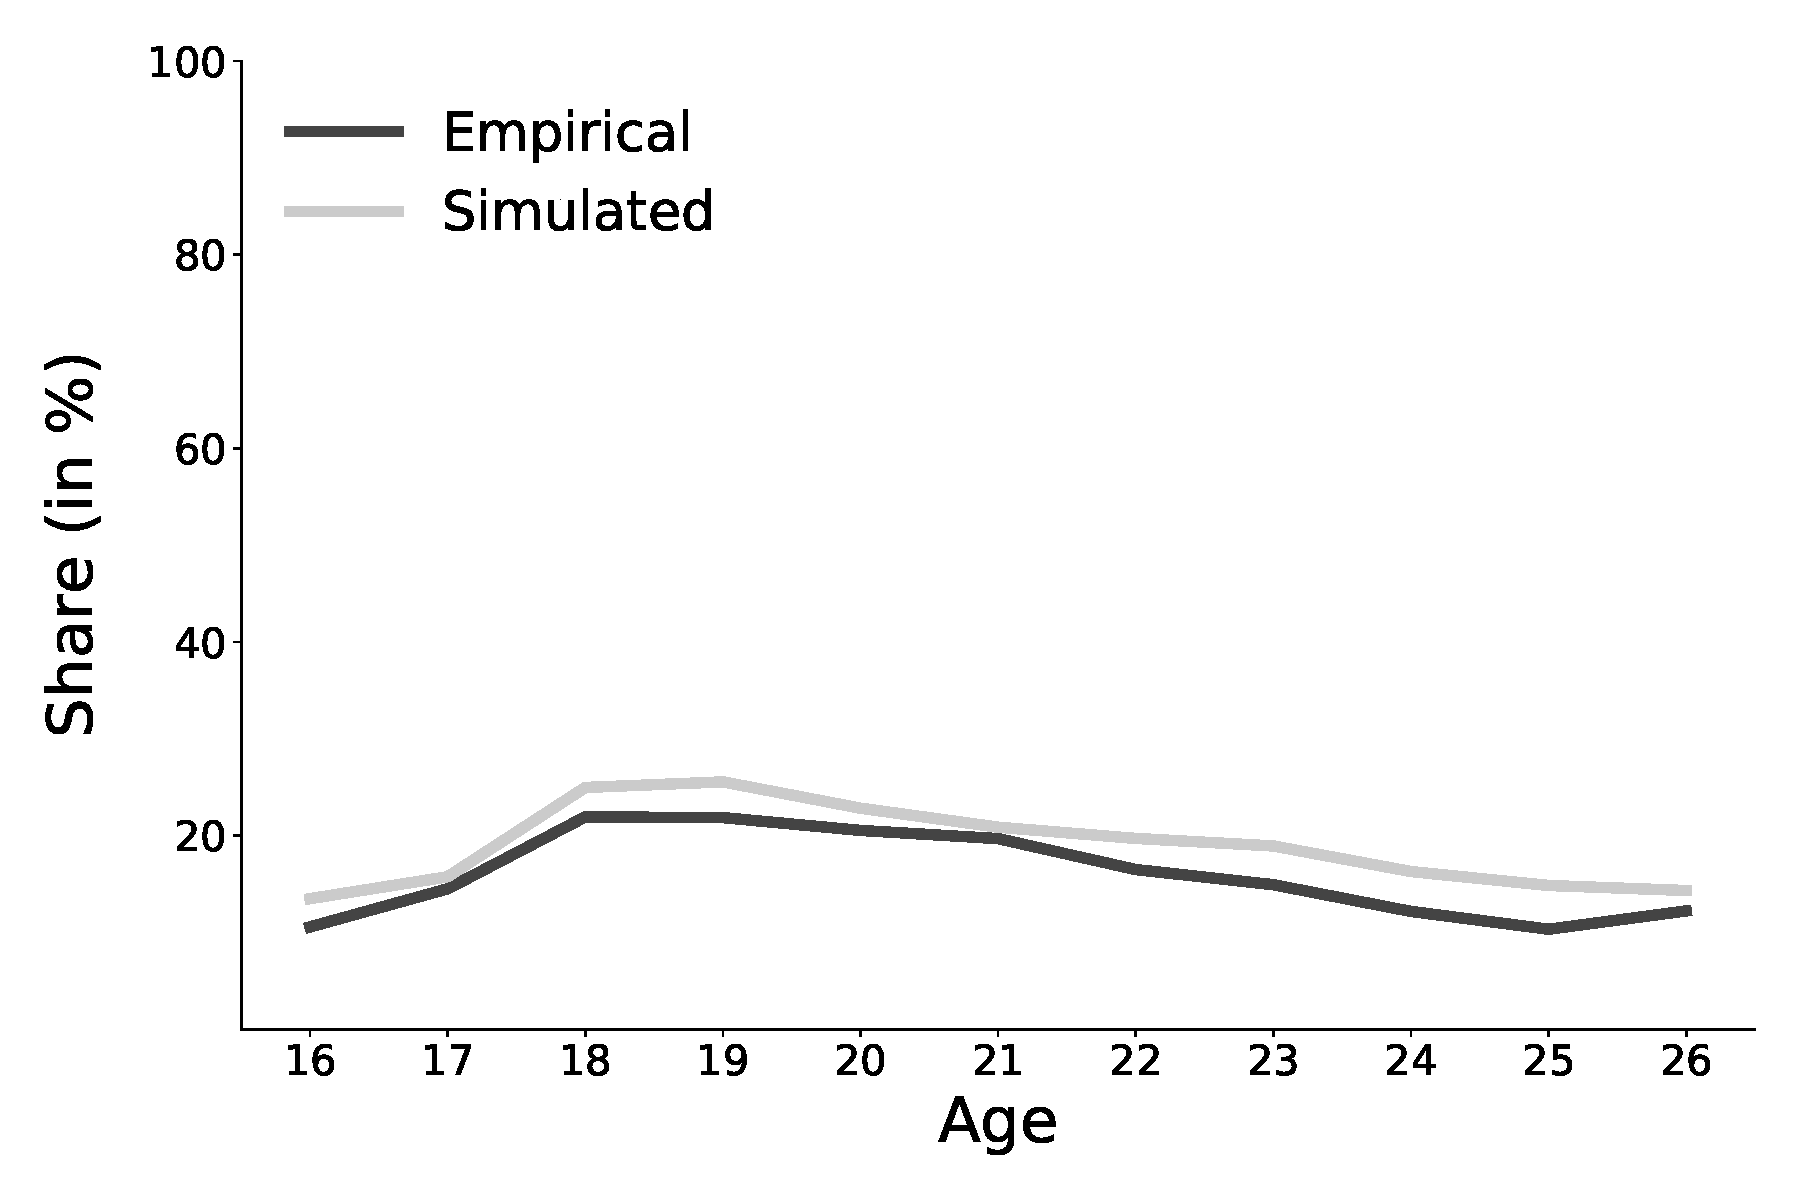
\includegraphics{fig-model-fit-choice-home-bw}}}
\end{figure}
\newpage

\end{appendices}

\end{document}
